\documentclass[twoside]{book}

% Packages required by doxygen
\usepackage{fixltx2e}
\usepackage{calc}
\usepackage{doxygen}
\usepackage[export]{adjustbox} % also loads graphicx
\usepackage{graphicx}
\usepackage[utf8]{inputenc}
\usepackage{makeidx}
\usepackage{multicol}
\usepackage{multirow}
\PassOptionsToPackage{warn}{textcomp}
\usepackage{textcomp}
\usepackage[nointegrals]{wasysym}
\usepackage[table]{xcolor}

% Font selection
\usepackage[T1]{fontenc}
\usepackage[scaled=.90]{helvet}
\usepackage{courier}
\usepackage{amssymb}
\usepackage{sectsty}
\renewcommand{\familydefault}{\sfdefault}
\allsectionsfont{%
  \fontseries{bc}\selectfont%
  \color{darkgray}%
}
\renewcommand{\DoxyLabelFont}{%
  \fontseries{bc}\selectfont%
  \color{darkgray}%
}
\newcommand{\+}{\discretionary{\mbox{\scriptsize$\hookleftarrow$}}{}{}}

% Page & text layout
\usepackage{geometry}
\geometry{%
  a4paper,%
  top=2.5cm,%
  bottom=2.5cm,%
  left=2.5cm,%
  right=2.5cm%
}
\tolerance=750
\hfuzz=15pt
\hbadness=750
\setlength{\emergencystretch}{15pt}
\setlength{\parindent}{0cm}
\setlength{\parskip}{0.2cm}
\makeatletter
\renewcommand{\paragraph}{%
  \@startsection{paragraph}{4}{0ex}{-1.0ex}{1.0ex}{%
    \normalfont\normalsize\bfseries\SS@parafont%
  }%
}
\renewcommand{\subparagraph}{%
  \@startsection{subparagraph}{5}{0ex}{-1.0ex}{1.0ex}{%
    \normalfont\normalsize\bfseries\SS@subparafont%
  }%
}
\makeatother

% Headers & footers
\usepackage{fancyhdr}
\pagestyle{fancyplain}
\fancyhead[LE]{\fancyplain{}{\bfseries\thepage}}
\fancyhead[CE]{\fancyplain{}{}}
\fancyhead[RE]{\fancyplain{}{\bfseries\leftmark}}
\fancyhead[LO]{\fancyplain{}{\bfseries\rightmark}}
\fancyhead[CO]{\fancyplain{}{}}
\fancyhead[RO]{\fancyplain{}{\bfseries\thepage}}
\fancyfoot[LE]{\fancyplain{}{}}
\fancyfoot[CE]{\fancyplain{}{}}
\fancyfoot[RE]{\fancyplain{}{\bfseries\scriptsize Generated on Wed Jun 22 2016 00\+:24\+:52 for surrive-\/the-\/map by Doxygen }}
\fancyfoot[LO]{\fancyplain{}{\bfseries\scriptsize Generated on Wed Jun 22 2016 00\+:24\+:52 for surrive-\/the-\/map by Doxygen }}
\fancyfoot[CO]{\fancyplain{}{}}
\fancyfoot[RO]{\fancyplain{}{}}
\renewcommand{\footrulewidth}{0.4pt}
\renewcommand{\chaptermark}[1]{%
  \markboth{#1}{}%
}
\renewcommand{\sectionmark}[1]{%
  \markright{\thesection\ #1}%
}

% Indices & bibliography
\usepackage{natbib}
\usepackage[titles]{tocloft}
\setcounter{tocdepth}{3}
\setcounter{secnumdepth}{5}
\makeindex

% Hyperlinks (required, but should be loaded last)
\usepackage{ifpdf}
\ifpdf
  \usepackage[pdftex,pagebackref=true]{hyperref}
\else
  \usepackage[ps2pdf,pagebackref=true]{hyperref}
\fi
\hypersetup{%
  colorlinks=true,%
  linkcolor=blue,%
  citecolor=blue,%
  unicode%
}

% Custom commands
\newcommand{\clearemptydoublepage}{%
  \newpage{\pagestyle{empty}\cleardoublepage}%
}


%===== C O N T E N T S =====

\begin{document}

% Titlepage & ToC
\hypersetup{pageanchor=false,
             bookmarks=true,
             bookmarksnumbered=true,
             pdfencoding=unicode
            }
\pagenumbering{roman}
\begin{titlepage}
\vspace*{7cm}
\begin{center}%
{\Large surrive-\/the-\/map \\[1ex]\large 0.\+01 }\\
\vspace*{1cm}
{\large Generated by Doxygen 1.8.9.1}\\
\vspace*{0.5cm}
{\small Wed Jun 22 2016 00:24:52}\\
\end{center}
\end{titlepage}
\clearemptydoublepage
\tableofcontents
\clearemptydoublepage
\pagenumbering{arabic}
\hypersetup{pageanchor=true}

%--- Begin generated contents ---
\chapter{Main Page}
\label{index}\hypertarget{index}{}Empty-\/\+S\+F\+M\+L project -\/ dll linking.\begin{DoxyNote}{Note}
with gh-\/pages \+:V
\end{DoxyNote}
\begin{DoxyAuthor}{Author}
Fotoblysk
\end{DoxyAuthor}
\begin{DoxyVersion}{Version}

\end{DoxyVersion}
\begin{DoxyParagraph}{Revision}
0.\+01 
\end{DoxyParagraph}


\begin{DoxyDate}{Date}
2016/03/13 21\+:44\+:00
\end{DoxyDate}
Contact\+: \href{mailto:fotoblysk@fejm.pl}{\tt fotoblysk@fejm.\+pl}

Created on\+: Sun Mar 13 21\+:44\+:00 2016

\begin{DoxyParagraph}{Id}
Empty-\/\+S\+F\+M\+L-\/dll,v 1.\+00 21\+:44\+:00 bv Exp Fotoblysk
\end{DoxyParagraph}

\chapter{surrive-\/the-\/map}
\label{md__c_1__users__foto__documents__git_hub_surrive-the-map__r_e_a_d_m_e}
\hypertarget{md__c_1__users__foto__documents__git_hub_surrive-the-map__r_e_a_d_m_e}{}
Simple game to get comfortable with design patterns and functional programming style. \hyperlink{class_game}{Game} ahve been written useing S\+F\+M\+L-\/2.\+3.\+2 libary -\/ dynamic linking, and Code\+::\+Blocks I\+D\+E. The game is originally made for a system Windows 8.\+1 64 bit, however compiled for 32 architecture. To\+Do list in \hyperlink{main_8cpp}{main.\+cpp} \#\+This branch is not ready to test, can have memory leaks, and may need refactoring. 
\chapter{Namespace Index}
\section{Namespace List}
Here is a list of all namespaces with brief descriptions\+:\begin{DoxyCompactList}
\item\contentsline{section}{\hyperlink{namespace_general_tools}{General\+Tools} }{\pageref{namespace_general_tools}}{}
\end{DoxyCompactList}

\chapter{Hierarchical Index}
\section{Class Hierarchy}
This inheritance list is sorted roughly, but not completely, alphabetically\+:\begin{DoxyCompactList}
\item Circle\+Shape\begin{DoxyCompactList}
\item \contentsline{section}{Bullet}{\pageref{class_bullet}}{}
\item \contentsline{section}{Enemy}{\pageref{class_enemy}}{}
\item \contentsline{section}{Player}{\pageref{class_player}}{}
\end{DoxyCompactList}
\item \contentsline{section}{Command}{\pageref{class_command}}{}
\begin{DoxyCompactList}
\item \contentsline{section}{Enter\+Choice\+Command}{\pageref{class_enter_choice_command}}{}
\item \contentsline{section}{Menu\+Command}{\pageref{class_menu_command}}{}
\item \contentsline{section}{Move\+Actor\+Command}{\pageref{class_move_actor_command}}{}
\item \contentsline{section}{Move\+Selection\+Command}{\pageref{class_move_selection_command}}{}
\item \contentsline{section}{Quit\+Game\+Command}{\pageref{class_quit_game_command}}{}
\item \contentsline{section}{Spawn\+Bullet\+Command}{\pageref{class_spawn_bullet_command}}{}
\item \contentsline{section}{Start\+Single\+Game\+Command}{\pageref{class_start_single_game_command}}{}
\end{DoxyCompactList}
\item \contentsline{section}{Enemy\+Spawner}{\pageref{class_enemy_spawner}}{}
\item \contentsline{section}{Engine}{\pageref{class_engine}}{}
\item \contentsline{section}{Game}{\pageref{class_game}}{}
\item \contentsline{section}{Game\+Object}{\pageref{class_game_object}}{}
\begin{DoxyCompactList}
\item \contentsline{section}{Actor}{\pageref{class_actor}}{}
\begin{DoxyCompactList}
\item \contentsline{section}{Enemy}{\pageref{class_enemy}}{}
\item \contentsline{section}{Player}{\pageref{class_player}}{}
\end{DoxyCompactList}
\item \contentsline{section}{Bullet}{\pageref{class_bullet}}{}
\end{DoxyCompactList}
\item \contentsline{section}{Input\+Handler}{\pageref{class_input_handler}}{}
\begin{DoxyCompactList}
\item \contentsline{section}{Ai\+Controler}{\pageref{class_ai_controler}}{}
\item \contentsline{section}{Collision\+Handler}{\pageref{class_collision_handler}}{}
\item \contentsline{section}{Engine\+Input\+Handler}{\pageref{class_engine_input_handler}}{}
\item \contentsline{section}{Menu\+Input\+Handler}{\pageref{class_menu_input_handler}}{}
\end{DoxyCompactList}
\item \contentsline{section}{Menu}{\pageref{class_menu}}{}
\begin{DoxyCompactList}
\item \contentsline{section}{Main\+Menu}{\pageref{class_main_menu}}{}
\end{DoxyCompactList}
\end{DoxyCompactList}

\chapter{Class Index}
\section{Class List}
Here are the classes, structs, unions and interfaces with brief descriptions\+:\begin{DoxyCompactList}
\item\contentsline{section}{\hyperlink{class_actor}{Actor} }{\pageref{class_actor}}{}
\item\contentsline{section}{\hyperlink{class_ai_controler}{Ai\+Controler} }{\pageref{class_ai_controler}}{}
\item\contentsline{section}{\hyperlink{class_bullet}{Bullet} }{\pageref{class_bullet}}{}
\item\contentsline{section}{\hyperlink{class_collision_handler}{Collision\+Handler} }{\pageref{class_collision_handler}}{}
\item\contentsline{section}{\hyperlink{class_command}{Command} }{\pageref{class_command}}{}
\item\contentsline{section}{\hyperlink{class_enemy}{Enemy} }{\pageref{class_enemy}}{}
\item\contentsline{section}{\hyperlink{class_enemy_spawner}{Enemy\+Spawner} }{\pageref{class_enemy_spawner}}{}
\item\contentsline{section}{\hyperlink{class_engine}{Engine} }{\pageref{class_engine}}{}
\item\contentsline{section}{\hyperlink{class_engine_input_handler}{Engine\+Input\+Handler} }{\pageref{class_engine_input_handler}}{}
\item\contentsline{section}{\hyperlink{class_enter_choice_command}{Enter\+Choice\+Command} }{\pageref{class_enter_choice_command}}{}
\item\contentsline{section}{\hyperlink{class_game}{Game} \\*\hyperlink{class_game}{Game} main class. Class which is used run engine. This class will menage menu and settings }{\pageref{class_game}}{}
\item\contentsline{section}{\hyperlink{class_game_object}{Game\+Object} }{\pageref{class_game_object}}{}
\item\contentsline{section}{\hyperlink{class_input_handler}{Input\+Handler} }{\pageref{class_input_handler}}{}
\item\contentsline{section}{\hyperlink{class_main_menu}{Main\+Menu} }{\pageref{class_main_menu}}{}
\item\contentsline{section}{\hyperlink{class_menu}{Menu} }{\pageref{class_menu}}{}
\item\contentsline{section}{\hyperlink{class_menu_command}{Menu\+Command} }{\pageref{class_menu_command}}{}
\item\contentsline{section}{\hyperlink{class_menu_input_handler}{Menu\+Input\+Handler} }{\pageref{class_menu_input_handler}}{}
\item\contentsline{section}{\hyperlink{class_move_actor_command}{Move\+Actor\+Command} }{\pageref{class_move_actor_command}}{}
\item\contentsline{section}{\hyperlink{class_move_selection_command}{Move\+Selection\+Command} }{\pageref{class_move_selection_command}}{}
\item\contentsline{section}{\hyperlink{class_player}{Player} }{\pageref{class_player}}{}
\item\contentsline{section}{\hyperlink{class_quit_game_command}{Quit\+Game\+Command} }{\pageref{class_quit_game_command}}{}
\item\contentsline{section}{\hyperlink{class_spawn_bullet_command}{Spawn\+Bullet\+Command} }{\pageref{class_spawn_bullet_command}}{}
\item\contentsline{section}{\hyperlink{class_start_single_game_command}{Start\+Single\+Game\+Command} }{\pageref{class_start_single_game_command}}{}
\end{DoxyCompactList}

\chapter{File Index}
\section{File List}
Here is a list of all files with brief descriptions\+:\begin{DoxyCompactList}
\item\contentsline{section}{\hyperlink{_actor_8cpp}{Actor.\+cpp} }{\pageref{_actor_8cpp}}{}
\item\contentsline{section}{\hyperlink{_actor_8h}{Actor.\+h} }{\pageref{_actor_8h}}{}
\item\contentsline{section}{\hyperlink{_ai_controler_8cpp}{Ai\+Controler.\+cpp} }{\pageref{_ai_controler_8cpp}}{}
\item\contentsline{section}{\hyperlink{_ai_controler_8h}{Ai\+Controler.\+h} }{\pageref{_ai_controler_8h}}{}
\item\contentsline{section}{\hyperlink{_bullet_8cpp}{Bullet.\+cpp} }{\pageref{_bullet_8cpp}}{}
\item\contentsline{section}{\hyperlink{_bullet_8h}{Bullet.\+h} }{\pageref{_bullet_8h}}{}
\item\contentsline{section}{\hyperlink{_collision_handler_8cpp}{Collision\+Handler.\+cpp} }{\pageref{_collision_handler_8cpp}}{}
\item\contentsline{section}{\hyperlink{_collision_handler_8h}{Collision\+Handler.\+h} }{\pageref{_collision_handler_8h}}{}
\item\contentsline{section}{\hyperlink{_command_8cpp}{Command.\+cpp} }{\pageref{_command_8cpp}}{}
\item\contentsline{section}{\hyperlink{_command_8h}{Command.\+h} }{\pageref{_command_8h}}{}
\item\contentsline{section}{\hyperlink{debugging__tolls_8h}{debugging\+\_\+tolls.\+h} \\*Personal debug macros. Include after defining N\+D\+E\+B\+U\+G to turn off }{\pageref{debugging__tolls_8h}}{}
\item\contentsline{section}{\hyperlink{_enemy_8cpp}{Enemy.\+cpp} }{\pageref{_enemy_8cpp}}{}
\item\contentsline{section}{\hyperlink{_enemy_8h}{Enemy.\+h} }{\pageref{_enemy_8h}}{}
\item\contentsline{section}{\hyperlink{_enemy_spawner_8cpp}{Enemy\+Spawner.\+cpp} }{\pageref{_enemy_spawner_8cpp}}{}
\item\contentsline{section}{\hyperlink{_enemy_spawner_8h}{Enemy\+Spawner.\+h} }{\pageref{_enemy_spawner_8h}}{}
\item\contentsline{section}{\hyperlink{_engine_8cpp}{Engine.\+cpp} }{\pageref{_engine_8cpp}}{}
\item\contentsline{section}{\hyperlink{_engine_8h}{Engine.\+h} }{\pageref{_engine_8h}}{}
\item\contentsline{section}{\hyperlink{_engine_input_handler_8cpp}{Engine\+Input\+Handler.\+cpp} }{\pageref{_engine_input_handler_8cpp}}{}
\item\contentsline{section}{\hyperlink{_engine_input_handler_8h}{Engine\+Input\+Handler.\+h} }{\pageref{_engine_input_handler_8h}}{}
\item\contentsline{section}{\hyperlink{_enter_choice_command_8cpp}{Enter\+Choice\+Command.\+cpp} }{\pageref{_enter_choice_command_8cpp}}{}
\item\contentsline{section}{\hyperlink{_enter_choice_command_8h}{Enter\+Choice\+Command.\+h} }{\pageref{_enter_choice_command_8h}}{}
\item\contentsline{section}{\hyperlink{_game_8cpp}{Game.\+cpp} }{\pageref{_game_8cpp}}{}
\item\contentsline{section}{\hyperlink{_game_8h}{Game.\+h} }{\pageref{_game_8h}}{}
\item\contentsline{section}{\hyperlink{_game_object_8cpp}{Game\+Object.\+cpp} }{\pageref{_game_object_8cpp}}{}
\item\contentsline{section}{\hyperlink{_game_object_8h}{Game\+Object.\+h} }{\pageref{_game_object_8h}}{}
\item\contentsline{section}{\hyperlink{_general_tools_8h}{General\+Tools.\+h} }{\pageref{_general_tools_8h}}{}
\item\contentsline{section}{\hyperlink{_input_handler_8cpp}{Input\+Handler.\+cpp} }{\pageref{_input_handler_8cpp}}{}
\item\contentsline{section}{\hyperlink{_input_handler_8h}{Input\+Handler.\+h} }{\pageref{_input_handler_8h}}{}
\item\contentsline{section}{\hyperlink{main_8cpp}{main.\+cpp} \\*Only \hyperlink{main_8cpp_ae66f6b31b5ad750f1fe042a706a4e3d4}{main()}. mainpage in }{\pageref{main_8cpp}}{}
\item\contentsline{section}{\hyperlink{_main_menu_8cpp}{Main\+Menu.\+cpp} }{\pageref{_main_menu_8cpp}}{}
\item\contentsline{section}{\hyperlink{_main_menu_8h}{Main\+Menu.\+h} }{\pageref{_main_menu_8h}}{}
\item\contentsline{section}{\hyperlink{_menu_8cpp}{Menu.\+cpp} }{\pageref{_menu_8cpp}}{}
\item\contentsline{section}{\hyperlink{_menu_8h}{Menu.\+h} }{\pageref{_menu_8h}}{}
\item\contentsline{section}{\hyperlink{_menu_command_8cpp}{Menu\+Command.\+cpp} }{\pageref{_menu_command_8cpp}}{}
\item\contentsline{section}{\hyperlink{_menu_command_8h}{Menu\+Command.\+h} }{\pageref{_menu_command_8h}}{}
\item\contentsline{section}{\hyperlink{_menu_input_handler_8cpp}{Menu\+Input\+Handler.\+cpp} }{\pageref{_menu_input_handler_8cpp}}{}
\item\contentsline{section}{\hyperlink{_menu_input_handler_8h}{Menu\+Input\+Handler.\+h} }{\pageref{_menu_input_handler_8h}}{}
\item\contentsline{section}{\hyperlink{_move_actor_command_8cpp}{Move\+Actor\+Command.\+cpp} }{\pageref{_move_actor_command_8cpp}}{}
\item\contentsline{section}{\hyperlink{_move_actor_command_8h}{Move\+Actor\+Command.\+h} }{\pageref{_move_actor_command_8h}}{}
\item\contentsline{section}{\hyperlink{_move_selection_command_8cpp}{Move\+Selection\+Command.\+cpp} }{\pageref{_move_selection_command_8cpp}}{}
\item\contentsline{section}{\hyperlink{_move_selection_command_8h}{Move\+Selection\+Command.\+h} }{\pageref{_move_selection_command_8h}}{}
\item\contentsline{section}{\hyperlink{_player_8cpp}{Player.\+cpp} }{\pageref{_player_8cpp}}{}
\item\contentsline{section}{\hyperlink{_player_8h}{Player.\+h} }{\pageref{_player_8h}}{}
\item\contentsline{section}{\hyperlink{_quit_game_command_8cpp}{Quit\+Game\+Command.\+cpp} }{\pageref{_quit_game_command_8cpp}}{}
\item\contentsline{section}{\hyperlink{_quit_game_command_8h}{Quit\+Game\+Command.\+h} }{\pageref{_quit_game_command_8h}}{}
\item\contentsline{section}{\hyperlink{_spawn_bullet_command_8cpp}{Spawn\+Bullet\+Command.\+cpp} }{\pageref{_spawn_bullet_command_8cpp}}{}
\item\contentsline{section}{\hyperlink{_spawn_bullet_command_8h}{Spawn\+Bullet\+Command.\+h} }{\pageref{_spawn_bullet_command_8h}}{}
\item\contentsline{section}{\hyperlink{_start_single_game_command_8cpp}{Start\+Single\+Game\+Command.\+cpp} }{\pageref{_start_single_game_command_8cpp}}{}
\item\contentsline{section}{\hyperlink{_start_single_game_command_8h}{Start\+Single\+Game\+Command.\+h} }{\pageref{_start_single_game_command_8h}}{}
\end{DoxyCompactList}

\chapter{Namespace Documentation}
\hypertarget{namespace_general_tools}{}\section{General\+Tools Namespace Reference}
\label{namespace_general_tools}\index{General\+Tools@{General\+Tools}}
\subsection*{Enumerations}
\begin{DoxyCompactItemize}
\item 
enum \hyperlink{namespace_general_tools_afedc3bd242369903830dec92c3ad569b}{Direction} \{ \hyperlink{namespace_general_tools_afedc3bd242369903830dec92c3ad569bab00acd9fb7b617ebfd46e4677100efed}{Left}, 
\hyperlink{namespace_general_tools_afedc3bd242369903830dec92c3ad569ba7775452bf315556da946fb19953566c6}{Right}, 
\hyperlink{namespace_general_tools_afedc3bd242369903830dec92c3ad569ba256487529104fc4bc5264d0ad0943cf1}{Up}, 
\hyperlink{namespace_general_tools_afedc3bd242369903830dec92c3ad569ba3a5a85a78f3258b606af0ce840a0b71e}{Down}
 \}
\end{DoxyCompactItemize}


\subsection{Enumeration Type Documentation}
\hypertarget{namespace_general_tools_afedc3bd242369903830dec92c3ad569b}{}\index{General\+Tools@{General\+Tools}!Direction@{Direction}}
\index{Direction@{Direction}!General\+Tools@{General\+Tools}}
\subsubsection[{Direction}]{\setlength{\rightskip}{0pt plus 5cm}enum {\bf General\+Tools\+::\+Direction}}\label{namespace_general_tools_afedc3bd242369903830dec92c3ad569b}
\begin{Desc}
\item[Enumerator]\par
\begin{description}
\index{Left@{Left}!General\+Tools@{General\+Tools}}\index{General\+Tools@{General\+Tools}!Left@{Left}}\item[{\em 
\hypertarget{namespace_general_tools_afedc3bd242369903830dec92c3ad569bab00acd9fb7b617ebfd46e4677100efed}{}Left\label{namespace_general_tools_afedc3bd242369903830dec92c3ad569bab00acd9fb7b617ebfd46e4677100efed}
}]\index{Right@{Right}!General\+Tools@{General\+Tools}}\index{General\+Tools@{General\+Tools}!Right@{Right}}\item[{\em 
\hypertarget{namespace_general_tools_afedc3bd242369903830dec92c3ad569ba7775452bf315556da946fb19953566c6}{}Right\label{namespace_general_tools_afedc3bd242369903830dec92c3ad569ba7775452bf315556da946fb19953566c6}
}]\index{Up@{Up}!General\+Tools@{General\+Tools}}\index{General\+Tools@{General\+Tools}!Up@{Up}}\item[{\em 
\hypertarget{namespace_general_tools_afedc3bd242369903830dec92c3ad569ba256487529104fc4bc5264d0ad0943cf1}{}Up\label{namespace_general_tools_afedc3bd242369903830dec92c3ad569ba256487529104fc4bc5264d0ad0943cf1}
}]\index{Down@{Down}!General\+Tools@{General\+Tools}}\index{General\+Tools@{General\+Tools}!Down@{Down}}\item[{\em 
\hypertarget{namespace_general_tools_afedc3bd242369903830dec92c3ad569ba3a5a85a78f3258b606af0ce840a0b71e}{}Down\label{namespace_general_tools_afedc3bd242369903830dec92c3ad569ba3a5a85a78f3258b606af0ce840a0b71e}
}]\end{description}
\end{Desc}

\chapter{Class Documentation}
\hypertarget{class_actor}{}\section{Actor Class Reference}
\label{class_actor}\index{Actor@{Actor}}


{\ttfamily \#include $<$Actor.\+h$>$}



Inheritance diagram for Actor\+:\nopagebreak
\begin{figure}[H]
\begin{center}
\leavevmode
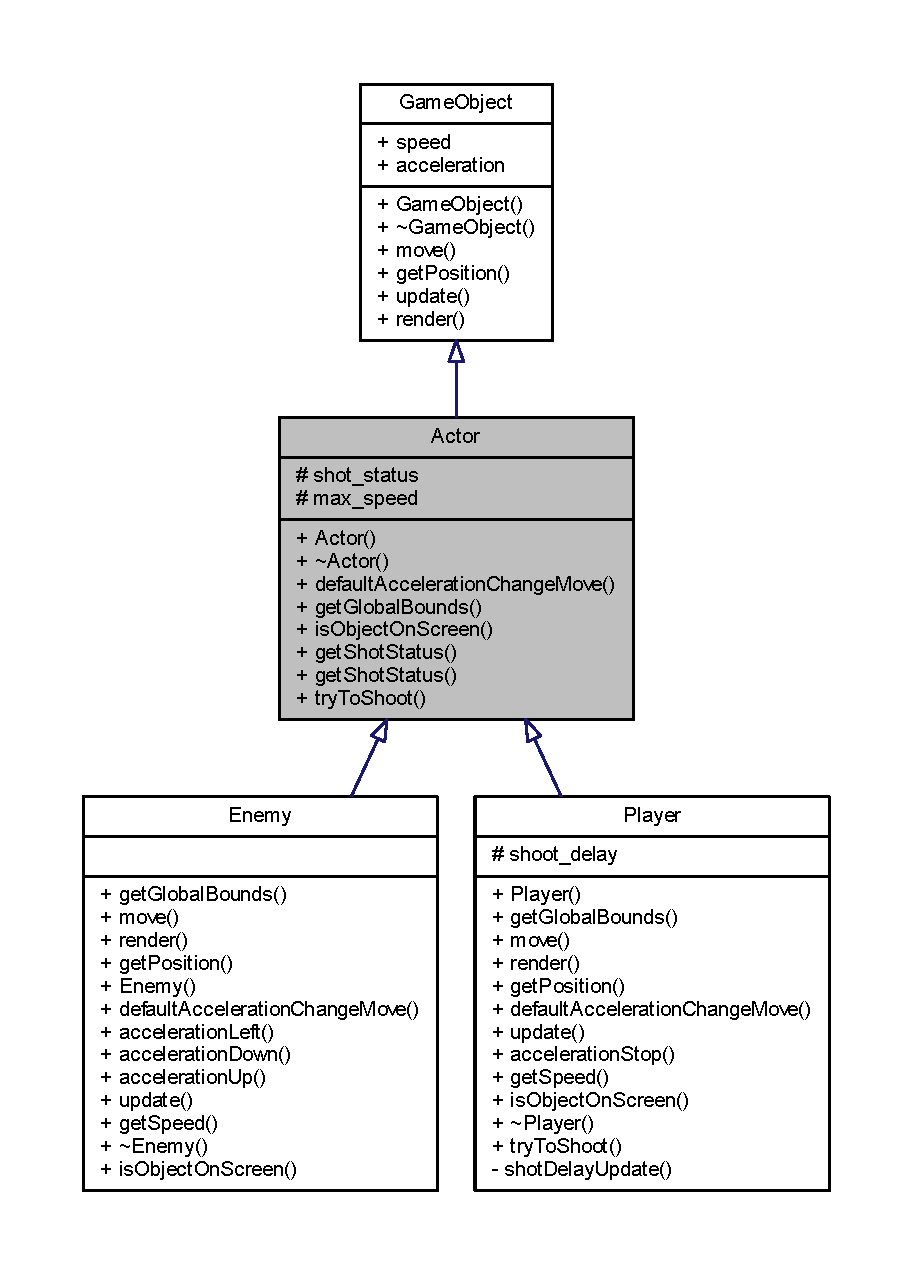
\includegraphics[width=350pt]{class_actor__inherit__graph}
\end{center}
\end{figure}


Collaboration diagram for Actor\+:\nopagebreak
\begin{figure}[H]
\begin{center}
\leavevmode
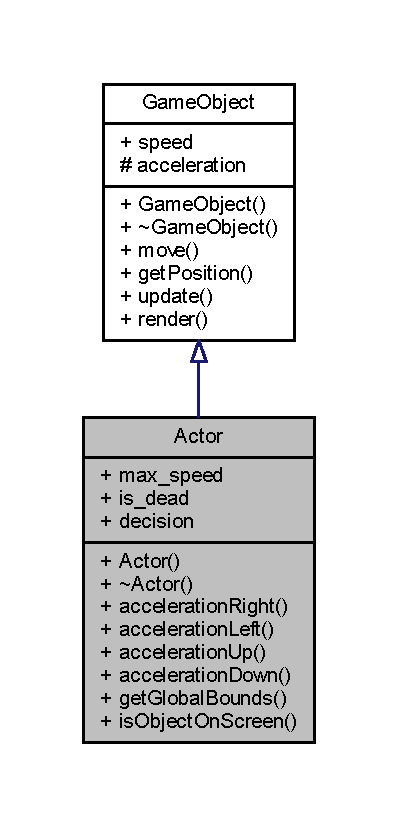
\includegraphics[width=250pt]{class_actor__coll__graph}
\end{center}
\end{figure}
\subsection*{Public Member Functions}
\begin{DoxyCompactItemize}
\item 
\hyperlink{class_actor_a2a0ff4335a1ee9096df90f288c026c8b}{Actor} ()
\item 
virtual \hyperlink{class_actor_ad807fe8f85e72ab263a0c05e3231cb39}{$\sim$\+Actor} ()
\item 
virtual void \hyperlink{class_actor_a9992ceb5499bff601e461c3bb93a8d48}{default\+Acceleration\+Change\+Move} (\hyperlink{namespace_general_tools_afedc3bd242369903830dec92c3ad569b}{General\+Tools\+::\+Direction} direction)=0
\item 
virtual sf\+::\+Float\+Rect \hyperlink{class_actor_ab56cff32076fef8392f4562fe281ea86}{get\+Global\+Bounds} ()=0
\item 
virtual bool \hyperlink{class_actor_a0bd104ef42ef1e3c3eea5c58e94c2429}{is\+Object\+On\+Screen} (sf\+::\+Render\+Window \&window)=0
\item 
virtual bool \hyperlink{class_actor_ad9cefebed5d4035bcf94c5a84dea21f9}{get\+Shot\+Status} () const 
\item 
virtual void \hyperlink{class_actor_a997ae7e0afe81e1423dd7135451be861}{get\+Shot\+Status} (bool new\+\_\+alive\+\_\+status)
\item 
virtual bool \hyperlink{class_actor_a85db8a17b338703247162f82f94cb957}{try\+To\+Shoot} ()
\end{DoxyCompactItemize}
\subsection*{Protected Attributes}
\begin{DoxyCompactItemize}
\item 
bool \hyperlink{class_actor_a675662b7b4e2c52a766ed4f460e18230}{shot\+\_\+status}
\item 
float \hyperlink{class_actor_a0adfb49f207e4a3e4f6b451da2a5b450}{max\+\_\+speed}
\end{DoxyCompactItemize}
\subsection*{Additional Inherited Members}


\subsection{Constructor \& Destructor Documentation}
\hypertarget{class_actor_a2a0ff4335a1ee9096df90f288c026c8b}{}\index{Actor@{Actor}!Actor@{Actor}}
\index{Actor@{Actor}!Actor@{Actor}}
\subsubsection[{Actor}]{\setlength{\rightskip}{0pt plus 5cm}Actor\+::\+Actor (
\begin{DoxyParamCaption}
{}
\end{DoxyParamCaption}
)\hspace{0.3cm}{\ttfamily [inline]}}\label{class_actor_a2a0ff4335a1ee9096df90f288c026c8b}
\hypertarget{class_actor_ad807fe8f85e72ab263a0c05e3231cb39}{}\index{Actor@{Actor}!````~Actor@{$\sim$\+Actor}}
\index{````~Actor@{$\sim$\+Actor}!Actor@{Actor}}
\subsubsection[{$\sim$\+Actor}]{\setlength{\rightskip}{0pt plus 5cm}Actor\+::$\sim$\+Actor (
\begin{DoxyParamCaption}
{}
\end{DoxyParamCaption}
)\hspace{0.3cm}{\ttfamily [virtual]}}\label{class_actor_ad807fe8f85e72ab263a0c05e3231cb39}


\subsection{Member Function Documentation}
\hypertarget{class_actor_a9992ceb5499bff601e461c3bb93a8d48}{}\index{Actor@{Actor}!default\+Acceleration\+Change\+Move@{default\+Acceleration\+Change\+Move}}
\index{default\+Acceleration\+Change\+Move@{default\+Acceleration\+Change\+Move}!Actor@{Actor}}
\subsubsection[{default\+Acceleration\+Change\+Move}]{\setlength{\rightskip}{0pt plus 5cm}virtual void Actor\+::default\+Acceleration\+Change\+Move (
\begin{DoxyParamCaption}
\item[{{\bf General\+Tools\+::\+Direction}}]{direction}
\end{DoxyParamCaption}
)\hspace{0.3cm}{\ttfamily [pure virtual]}}\label{class_actor_a9992ceb5499bff601e461c3bb93a8d48}


Implemented in \hyperlink{class_enemy_ae642ab230b9b416142cfe2a6ed3e3aeb}{Enemy}, and \hyperlink{class_player_a48e3ad0f384cd58a64136a40d4a04b76}{Player}.



Here is the caller graph for this function\+:\nopagebreak
\begin{figure}[H]
\begin{center}
\leavevmode
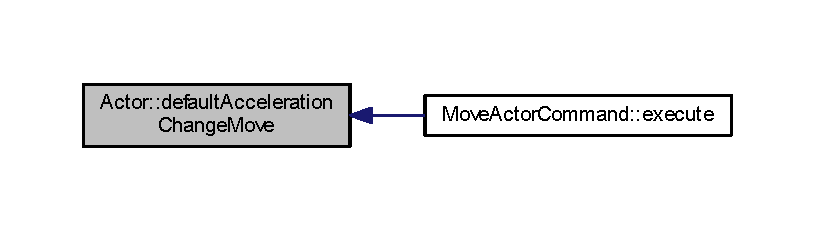
\includegraphics[width=350pt]{class_actor_a9992ceb5499bff601e461c3bb93a8d48_icgraph}
\end{center}
\end{figure}


\hypertarget{class_actor_ab56cff32076fef8392f4562fe281ea86}{}\index{Actor@{Actor}!get\+Global\+Bounds@{get\+Global\+Bounds}}
\index{get\+Global\+Bounds@{get\+Global\+Bounds}!Actor@{Actor}}
\subsubsection[{get\+Global\+Bounds}]{\setlength{\rightskip}{0pt plus 5cm}virtual sf\+::\+Float\+Rect Actor\+::get\+Global\+Bounds (
\begin{DoxyParamCaption}
{}
\end{DoxyParamCaption}
)\hspace{0.3cm}{\ttfamily [pure virtual]}}\label{class_actor_ab56cff32076fef8392f4562fe281ea86}


Implemented in \hyperlink{class_player_ac2b21f8a74b6b1c0e9068a82e7e71e86}{Player}, and \hyperlink{class_enemy_abb50439b9517d5a2b4c6b6c6a4e91672}{Enemy}.



Here is the caller graph for this function\+:\nopagebreak
\begin{figure}[H]
\begin{center}
\leavevmode
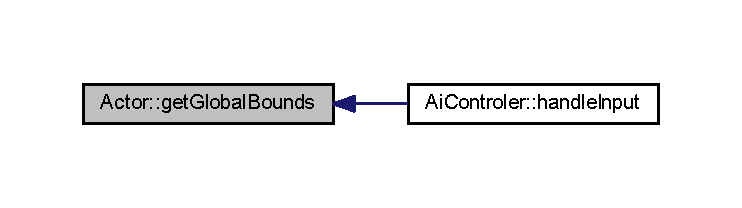
\includegraphics[width=350pt]{class_actor_ab56cff32076fef8392f4562fe281ea86_icgraph}
\end{center}
\end{figure}


\hypertarget{class_actor_ad9cefebed5d4035bcf94c5a84dea21f9}{}\index{Actor@{Actor}!get\+Shot\+Status@{get\+Shot\+Status}}
\index{get\+Shot\+Status@{get\+Shot\+Status}!Actor@{Actor}}
\subsubsection[{get\+Shot\+Status}]{\setlength{\rightskip}{0pt plus 5cm}bool Actor\+::get\+Shot\+Status (
\begin{DoxyParamCaption}
{}
\end{DoxyParamCaption}
) const\hspace{0.3cm}{\ttfamily [virtual]}}\label{class_actor_ad9cefebed5d4035bcf94c5a84dea21f9}


Here is the caller graph for this function\+:\nopagebreak
\begin{figure}[H]
\begin{center}
\leavevmode
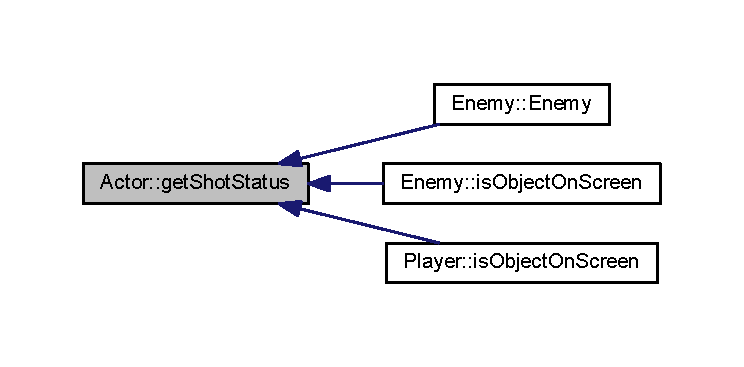
\includegraphics[width=350pt]{class_actor_ad9cefebed5d4035bcf94c5a84dea21f9_icgraph}
\end{center}
\end{figure}


\hypertarget{class_actor_a997ae7e0afe81e1423dd7135451be861}{}\index{Actor@{Actor}!get\+Shot\+Status@{get\+Shot\+Status}}
\index{get\+Shot\+Status@{get\+Shot\+Status}!Actor@{Actor}}
\subsubsection[{get\+Shot\+Status}]{\setlength{\rightskip}{0pt plus 5cm}void Actor\+::get\+Shot\+Status (
\begin{DoxyParamCaption}
\item[{bool}]{new\+\_\+alive\+\_\+status}
\end{DoxyParamCaption}
)\hspace{0.3cm}{\ttfamily [virtual]}}\label{class_actor_a997ae7e0afe81e1423dd7135451be861}
\hypertarget{class_actor_a0bd104ef42ef1e3c3eea5c58e94c2429}{}\index{Actor@{Actor}!is\+Object\+On\+Screen@{is\+Object\+On\+Screen}}
\index{is\+Object\+On\+Screen@{is\+Object\+On\+Screen}!Actor@{Actor}}
\subsubsection[{is\+Object\+On\+Screen}]{\setlength{\rightskip}{0pt plus 5cm}virtual bool Actor\+::is\+Object\+On\+Screen (
\begin{DoxyParamCaption}
\item[{sf\+::\+Render\+Window \&}]{window}
\end{DoxyParamCaption}
)\hspace{0.3cm}{\ttfamily [pure virtual]}}\label{class_actor_a0bd104ef42ef1e3c3eea5c58e94c2429}


Implemented in \hyperlink{class_enemy_a9a6b7416616b3d0464978d38cf7095e9}{Enemy}, and \hyperlink{class_player_ac2c0f9ac6f1d4908465a23f9ddb4cb1c}{Player}.

\hypertarget{class_actor_a85db8a17b338703247162f82f94cb957}{}\index{Actor@{Actor}!try\+To\+Shoot@{try\+To\+Shoot}}
\index{try\+To\+Shoot@{try\+To\+Shoot}!Actor@{Actor}}
\subsubsection[{try\+To\+Shoot}]{\setlength{\rightskip}{0pt plus 5cm}virtual bool Actor\+::try\+To\+Shoot (
\begin{DoxyParamCaption}
{}
\end{DoxyParamCaption}
)\hspace{0.3cm}{\ttfamily [inline]}, {\ttfamily [virtual]}}\label{class_actor_a85db8a17b338703247162f82f94cb957}


Reimplemented in \hyperlink{class_player_a52486292c25bc6ac6589423ef0c81b0e}{Player}.



\subsection{Member Data Documentation}
\hypertarget{class_actor_a0adfb49f207e4a3e4f6b451da2a5b450}{}\index{Actor@{Actor}!max\+\_\+speed@{max\+\_\+speed}}
\index{max\+\_\+speed@{max\+\_\+speed}!Actor@{Actor}}
\subsubsection[{max\+\_\+speed}]{\setlength{\rightskip}{0pt plus 5cm}float Actor\+::max\+\_\+speed\hspace{0.3cm}{\ttfamily [protected]}}\label{class_actor_a0adfb49f207e4a3e4f6b451da2a5b450}
\hypertarget{class_actor_a675662b7b4e2c52a766ed4f460e18230}{}\index{Actor@{Actor}!shot\+\_\+status@{shot\+\_\+status}}
\index{shot\+\_\+status@{shot\+\_\+status}!Actor@{Actor}}
\subsubsection[{shot\+\_\+status}]{\setlength{\rightskip}{0pt plus 5cm}bool Actor\+::shot\+\_\+status\hspace{0.3cm}{\ttfamily [protected]}}\label{class_actor_a675662b7b4e2c52a766ed4f460e18230}


The documentation for this class was generated from the following files\+:\begin{DoxyCompactItemize}
\item 
\hyperlink{_actor_8h}{Actor.\+h}\item 
\hyperlink{_actor_8cpp}{Actor.\+cpp}\end{DoxyCompactItemize}

\hypertarget{class_ai_controler}{}\section{Ai\+Controler Class Reference}
\label{class_ai_controler}\index{Ai\+Controler@{Ai\+Controler}}


{\ttfamily \#include $<$Ai\+Controler.\+h$>$}



Inheritance diagram for Ai\+Controler\+:\nopagebreak
\begin{figure}[H]
\begin{center}
\leavevmode
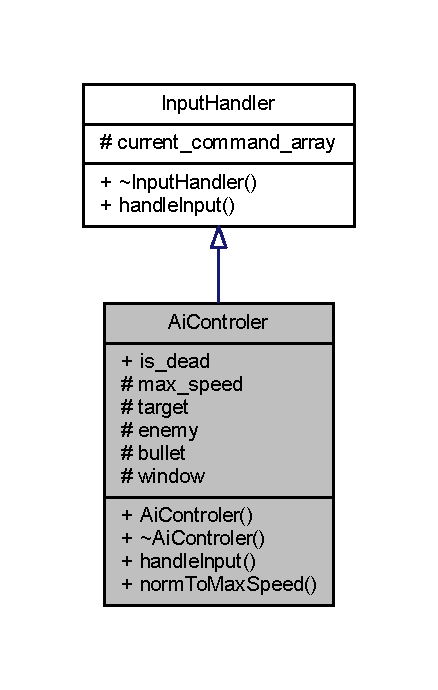
\includegraphics[width=210pt]{class_ai_controler__inherit__graph}
\end{center}
\end{figure}


Collaboration diagram for Ai\+Controler\+:\nopagebreak
\begin{figure}[H]
\begin{center}
\leavevmode
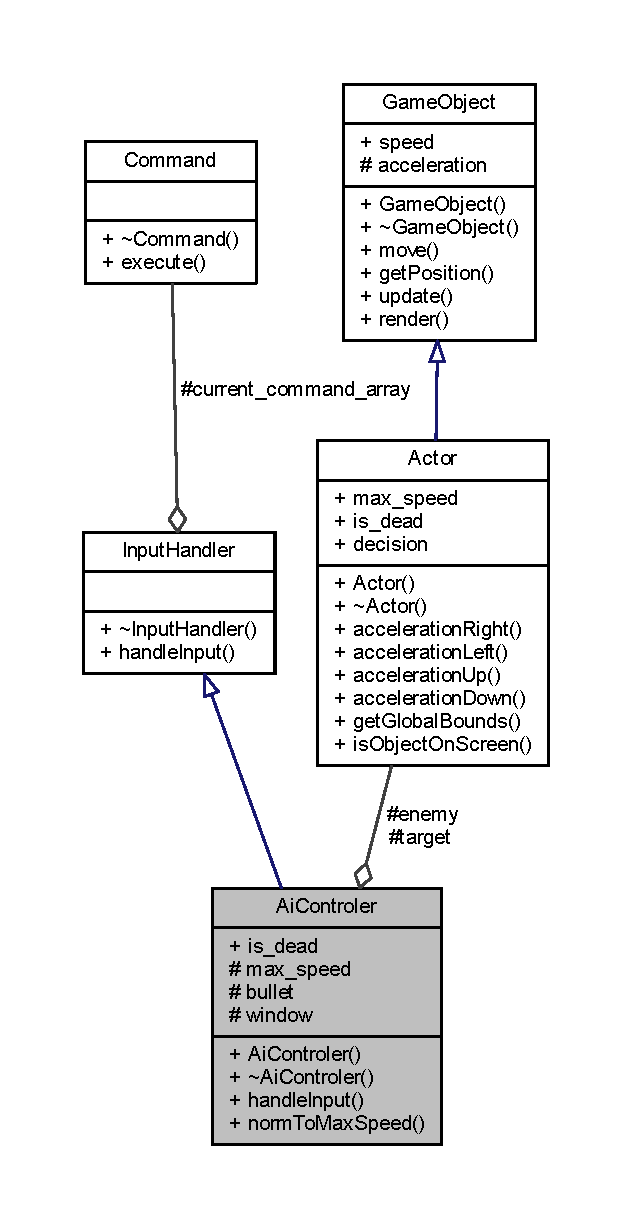
\includegraphics[height=550pt]{class_ai_controler__coll__graph}
\end{center}
\end{figure}
\subsection*{Public Member Functions}
\begin{DoxyCompactItemize}
\item 
\hyperlink{class_ai_controler_a33bdaad21e07f2d93ae0ea277035193b}{Ai\+Controler} (\hyperlink{class_actor}{Actor} $\ast$\&target\+\_\+in, \hyperlink{class_actor}{Actor} $\ast$\&enemy\+\_\+in, std\+::vector$<$ \hyperlink{class_bullet}{Bullet} $\ast$ $>$ \&bullet\+\_\+in, sf\+::\+Render\+Window \&window\+\_\+in)
\item 
virtual \hyperlink{class_ai_controler_aa58de5f8ccbff5d293c57cdf2a80e8c5}{$\sim$\+Ai\+Controler} ()
\item 
\hyperlink{class_command}{Command} $\ast$$\ast$ \hyperlink{class_ai_controler_a72891536d5ff122ae1e3a25fd62fd1b5}{handle\+Input} ()
\end{DoxyCompactItemize}
\subsection*{Private Member Functions}
\begin{DoxyCompactItemize}
\item 
sf\+::\+Vector2f \hyperlink{class_ai_controler_aa388145d3791cd80b1d53a5847428f68}{norm\+To\+Max\+Speed} (sf\+::\+Vector2f in\+\_\+vector, const float \&gain)
\end{DoxyCompactItemize}
\subsection*{Private Attributes}
\begin{DoxyCompactItemize}
\item 
bool \hyperlink{class_ai_controler_aaf7042b1051e301b6b356bc6d702dccd}{is\+\_\+dead}
\item 
float \hyperlink{class_ai_controler_ab541f013a1b6ba763ec1bc4c183816d0}{max\+\_\+speed}
\item 
\hyperlink{class_actor}{Actor} $\ast$ \hyperlink{class_ai_controler_aa0130bc7fd057f94accf3aa3d542173b}{target}
\item 
\hyperlink{class_actor}{Actor} $\ast$ \hyperlink{class_ai_controler_a71e4c6c84203c1b50b6e1d55b582db62}{enemy}
\item 
std\+::vector$<$ \hyperlink{class_bullet}{Bullet} $\ast$ $>$ \& \hyperlink{class_ai_controler_a11a907d64a91c99ca5df9a908c1fdad7}{bullet}
\item 
sf\+::\+Render\+Window \& \hyperlink{class_ai_controler_ac352e418d681e34fb822a1d70c84fb05}{window}
\item 
int \hyperlink{class_ai_controler_a8d44859dfa97e10f04c532a0f2d69bfb}{decision}
\end{DoxyCompactItemize}
\subsection*{Additional Inherited Members}


\subsection{Constructor \& Destructor Documentation}
\hypertarget{class_ai_controler_a33bdaad21e07f2d93ae0ea277035193b}{}\index{Ai\+Controler@{Ai\+Controler}!Ai\+Controler@{Ai\+Controler}}
\index{Ai\+Controler@{Ai\+Controler}!Ai\+Controler@{Ai\+Controler}}
\subsubsection[{Ai\+Controler}]{\setlength{\rightskip}{0pt plus 5cm}Ai\+Controler\+::\+Ai\+Controler (
\begin{DoxyParamCaption}
\item[{{\bf Actor} $\ast$\&}]{target\+\_\+in, }
\item[{{\bf Actor} $\ast$\&}]{enemy\+\_\+in, }
\item[{std\+::vector$<$ {\bf Bullet} $\ast$ $>$ \&}]{bullet\+\_\+in, }
\item[{sf\+::\+Render\+Window \&}]{window\+\_\+in}
\end{DoxyParamCaption}
)}\label{class_ai_controler_a33bdaad21e07f2d93ae0ea277035193b}
\hypertarget{class_ai_controler_aa58de5f8ccbff5d293c57cdf2a80e8c5}{}\index{Ai\+Controler@{Ai\+Controler}!````~Ai\+Controler@{$\sim$\+Ai\+Controler}}
\index{````~Ai\+Controler@{$\sim$\+Ai\+Controler}!Ai\+Controler@{Ai\+Controler}}
\subsubsection[{$\sim$\+Ai\+Controler}]{\setlength{\rightskip}{0pt plus 5cm}Ai\+Controler\+::$\sim$\+Ai\+Controler (
\begin{DoxyParamCaption}
{}
\end{DoxyParamCaption}
)\hspace{0.3cm}{\ttfamily [virtual]}}\label{class_ai_controler_aa58de5f8ccbff5d293c57cdf2a80e8c5}


\subsection{Member Function Documentation}
\hypertarget{class_ai_controler_a72891536d5ff122ae1e3a25fd62fd1b5}{}\index{Ai\+Controler@{Ai\+Controler}!handle\+Input@{handle\+Input}}
\index{handle\+Input@{handle\+Input}!Ai\+Controler@{Ai\+Controler}}
\subsubsection[{handle\+Input}]{\setlength{\rightskip}{0pt plus 5cm}{\bf Command} $\ast$$\ast$ Ai\+Controler\+::handle\+Input (
\begin{DoxyParamCaption}
{}
\end{DoxyParamCaption}
)\hspace{0.3cm}{\ttfamily [virtual]}}\label{class_ai_controler_a72891536d5ff122ae1e3a25fd62fd1b5}


Implements \hyperlink{class_input_handler_a69b726d4a409a6f4ae443689cb69b404}{Input\+Handler}.



Here is the call graph for this function\+:\nopagebreak
\begin{figure}[H]
\begin{center}
\leavevmode
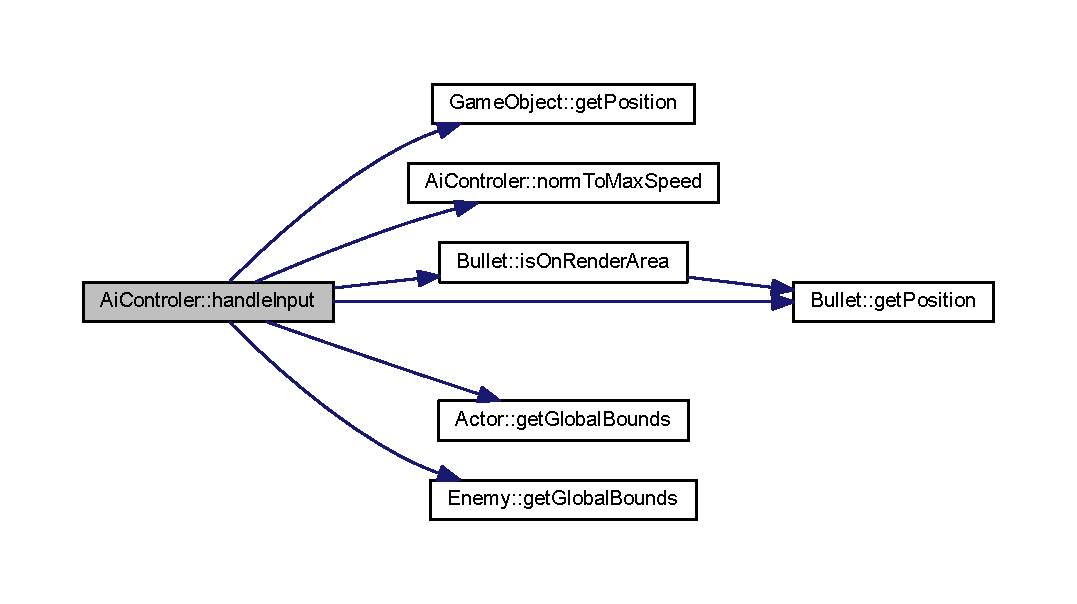
\includegraphics[width=350pt]{class_ai_controler_a72891536d5ff122ae1e3a25fd62fd1b5_cgraph}
\end{center}
\end{figure}


\hypertarget{class_ai_controler_aa388145d3791cd80b1d53a5847428f68}{}\index{Ai\+Controler@{Ai\+Controler}!norm\+To\+Max\+Speed@{norm\+To\+Max\+Speed}}
\index{norm\+To\+Max\+Speed@{norm\+To\+Max\+Speed}!Ai\+Controler@{Ai\+Controler}}
\subsubsection[{norm\+To\+Max\+Speed}]{\setlength{\rightskip}{0pt plus 5cm}sf\+::\+Vector2f Ai\+Controler\+::norm\+To\+Max\+Speed (
\begin{DoxyParamCaption}
\item[{sf\+::\+Vector2f}]{in\+\_\+vector, }
\item[{const float \&}]{gain}
\end{DoxyParamCaption}
)\hspace{0.3cm}{\ttfamily [private]}}\label{class_ai_controler_aa388145d3791cd80b1d53a5847428f68}


Here is the caller graph for this function\+:\nopagebreak
\begin{figure}[H]
\begin{center}
\leavevmode
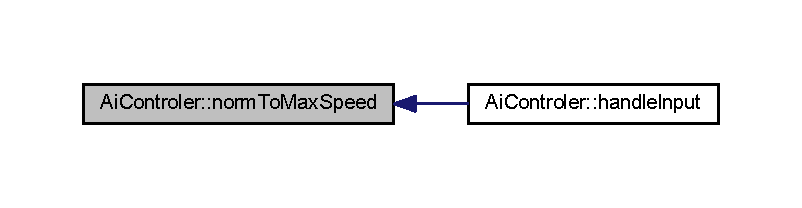
\includegraphics[width=350pt]{class_ai_controler_aa388145d3791cd80b1d53a5847428f68_icgraph}
\end{center}
\end{figure}




\subsection{Member Data Documentation}
\hypertarget{class_ai_controler_a11a907d64a91c99ca5df9a908c1fdad7}{}\index{Ai\+Controler@{Ai\+Controler}!bullet@{bullet}}
\index{bullet@{bullet}!Ai\+Controler@{Ai\+Controler}}
\subsubsection[{bullet}]{\setlength{\rightskip}{0pt plus 5cm}std\+::vector$<${\bf Bullet}$\ast$$>$\& Ai\+Controler\+::bullet\hspace{0.3cm}{\ttfamily [private]}}\label{class_ai_controler_a11a907d64a91c99ca5df9a908c1fdad7}
\hypertarget{class_ai_controler_a8d44859dfa97e10f04c532a0f2d69bfb}{}\index{Ai\+Controler@{Ai\+Controler}!decision@{decision}}
\index{decision@{decision}!Ai\+Controler@{Ai\+Controler}}
\subsubsection[{decision}]{\setlength{\rightskip}{0pt plus 5cm}int Ai\+Controler\+::decision\hspace{0.3cm}{\ttfamily [private]}}\label{class_ai_controler_a8d44859dfa97e10f04c532a0f2d69bfb}
\hypertarget{class_ai_controler_a71e4c6c84203c1b50b6e1d55b582db62}{}\index{Ai\+Controler@{Ai\+Controler}!enemy@{enemy}}
\index{enemy@{enemy}!Ai\+Controler@{Ai\+Controler}}
\subsubsection[{enemy}]{\setlength{\rightskip}{0pt plus 5cm}{\bf Actor}$\ast$ Ai\+Controler\+::enemy\hspace{0.3cm}{\ttfamily [private]}}\label{class_ai_controler_a71e4c6c84203c1b50b6e1d55b582db62}
\hypertarget{class_ai_controler_aaf7042b1051e301b6b356bc6d702dccd}{}\index{Ai\+Controler@{Ai\+Controler}!is\+\_\+dead@{is\+\_\+dead}}
\index{is\+\_\+dead@{is\+\_\+dead}!Ai\+Controler@{Ai\+Controler}}
\subsubsection[{is\+\_\+dead}]{\setlength{\rightskip}{0pt plus 5cm}bool Ai\+Controler\+::is\+\_\+dead\hspace{0.3cm}{\ttfamily [private]}}\label{class_ai_controler_aaf7042b1051e301b6b356bc6d702dccd}
\hypertarget{class_ai_controler_ab541f013a1b6ba763ec1bc4c183816d0}{}\index{Ai\+Controler@{Ai\+Controler}!max\+\_\+speed@{max\+\_\+speed}}
\index{max\+\_\+speed@{max\+\_\+speed}!Ai\+Controler@{Ai\+Controler}}
\subsubsection[{max\+\_\+speed}]{\setlength{\rightskip}{0pt plus 5cm}float Ai\+Controler\+::max\+\_\+speed\hspace{0.3cm}{\ttfamily [private]}}\label{class_ai_controler_ab541f013a1b6ba763ec1bc4c183816d0}
\hypertarget{class_ai_controler_aa0130bc7fd057f94accf3aa3d542173b}{}\index{Ai\+Controler@{Ai\+Controler}!target@{target}}
\index{target@{target}!Ai\+Controler@{Ai\+Controler}}
\subsubsection[{target}]{\setlength{\rightskip}{0pt plus 5cm}{\bf Actor}$\ast$ Ai\+Controler\+::target\hspace{0.3cm}{\ttfamily [private]}}\label{class_ai_controler_aa0130bc7fd057f94accf3aa3d542173b}
\hypertarget{class_ai_controler_ac352e418d681e34fb822a1d70c84fb05}{}\index{Ai\+Controler@{Ai\+Controler}!window@{window}}
\index{window@{window}!Ai\+Controler@{Ai\+Controler}}
\subsubsection[{window}]{\setlength{\rightskip}{0pt plus 5cm}sf\+::\+Render\+Window\& Ai\+Controler\+::window\hspace{0.3cm}{\ttfamily [private]}}\label{class_ai_controler_ac352e418d681e34fb822a1d70c84fb05}


The documentation for this class was generated from the following files\+:\begin{DoxyCompactItemize}
\item 
\hyperlink{_ai_controler_8h}{Ai\+Controler.\+h}\item 
\hyperlink{_ai_controler_8cpp}{Ai\+Controler.\+cpp}\end{DoxyCompactItemize}

\hypertarget{class_bullet}{}\section{Bullet Class Reference}
\label{class_bullet}\index{Bullet@{Bullet}}


{\ttfamily \#include $<$Bullet.\+h$>$}



Inheritance diagram for Bullet\+:
\nopagebreak
\begin{figure}[H]
\begin{center}
\leavevmode
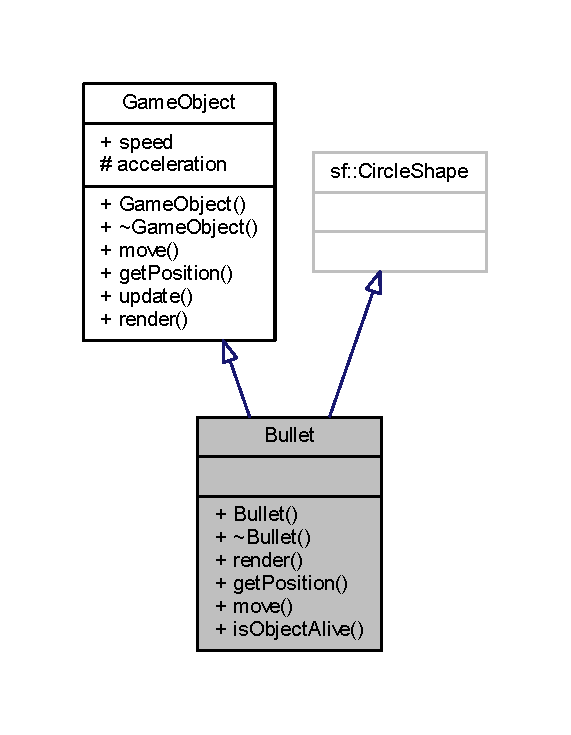
\includegraphics[width=274pt]{class_bullet__inherit__graph}
\end{center}
\end{figure}


Collaboration diagram for Bullet\+:
\nopagebreak
\begin{figure}[H]
\begin{center}
\leavevmode
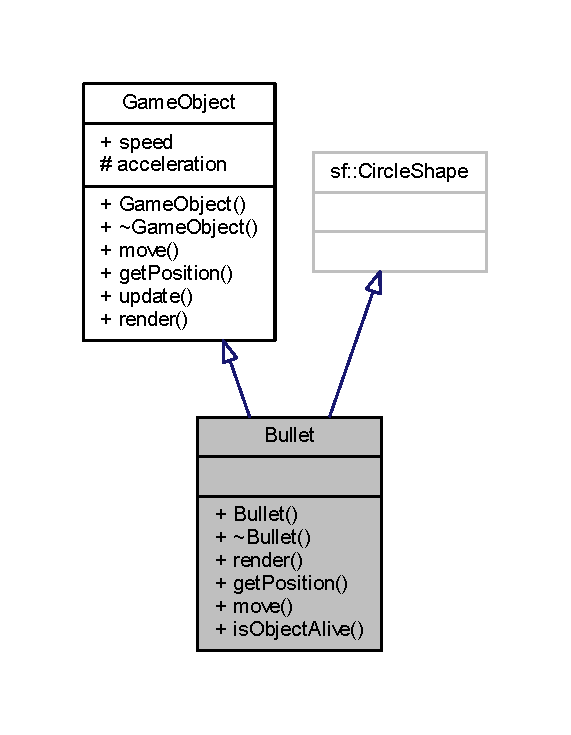
\includegraphics[width=274pt]{class_bullet__coll__graph}
\end{center}
\end{figure}
\subsection*{Public Member Functions}
\begin{DoxyCompactItemize}
\item 
\hyperlink{class_bullet_ab785558b82bce3c860a9d0f63aff2f41}{Bullet} (sf\+::\+Vector2f position\+\_\+in, sf\+::\+Vector2f speed\+\_\+in)
\item 
virtual \hyperlink{class_bullet_aaeb5cb41d7db89f49007b08b41f1bfcf}{$\sim$\+Bullet} ()
\item 
void \hyperlink{class_bullet_ae4af350647e1b2a798eb3fd35a883b84}{render} (sf\+::\+Render\+Window \&window) override
\item 
const sf\+::\+Vector2f \& \hyperlink{class_bullet_a82f82d6367d1c403898a29d1ce91630d}{get\+Position} () override
\item 
void \hyperlink{class_bullet_a8715ab2edff76c8b45fabc6dc453e85d}{move} (const sf\+::\+Vector2f \&offset) override
\item 
bool \hyperlink{class_bullet_a23cadfbb18a562482f0bae03f0edd029}{is\+Object\+Alive} (sf\+::\+Render\+Window \&window)
\end{DoxyCompactItemize}
\subsection*{Additional Inherited Members}


\subsection{Constructor \& Destructor Documentation}
\hypertarget{class_bullet_ab785558b82bce3c860a9d0f63aff2f41}{}\index{Bullet@{Bullet}!Bullet@{Bullet}}
\index{Bullet@{Bullet}!Bullet@{Bullet}}
\subsubsection[{Bullet}]{\setlength{\rightskip}{0pt plus 5cm}Bullet\+::\+Bullet (
\begin{DoxyParamCaption}
\item[{sf\+::\+Vector2f}]{position\+\_\+in, }
\item[{sf\+::\+Vector2f}]{speed\+\_\+in}
\end{DoxyParamCaption}
)}\label{class_bullet_ab785558b82bce3c860a9d0f63aff2f41}
\hypertarget{class_bullet_aaeb5cb41d7db89f49007b08b41f1bfcf}{}\index{Bullet@{Bullet}!````~Bullet@{$\sim$\+Bullet}}
\index{````~Bullet@{$\sim$\+Bullet}!Bullet@{Bullet}}
\subsubsection[{$\sim$\+Bullet}]{\setlength{\rightskip}{0pt plus 5cm}Bullet\+::$\sim$\+Bullet (
\begin{DoxyParamCaption}
{}
\end{DoxyParamCaption}
)\hspace{0.3cm}{\ttfamily [virtual]}}\label{class_bullet_aaeb5cb41d7db89f49007b08b41f1bfcf}


\subsection{Member Function Documentation}
\hypertarget{class_bullet_a82f82d6367d1c403898a29d1ce91630d}{}\index{Bullet@{Bullet}!get\+Position@{get\+Position}}
\index{get\+Position@{get\+Position}!Bullet@{Bullet}}
\subsubsection[{get\+Position}]{\setlength{\rightskip}{0pt plus 5cm}const sf\+::\+Vector2f\& Bullet\+::get\+Position (
\begin{DoxyParamCaption}
{}
\end{DoxyParamCaption}
)\hspace{0.3cm}{\ttfamily [inline]}, {\ttfamily [override]}, {\ttfamily [virtual]}}\label{class_bullet_a82f82d6367d1c403898a29d1ce91630d}


Implements \hyperlink{class_game_object_a3c1da4d2eaaf8384f3ca10735673991e}{Game\+Object}.



Here is the caller graph for this function\+:
\nopagebreak
\begin{figure}[H]
\begin{center}
\leavevmode
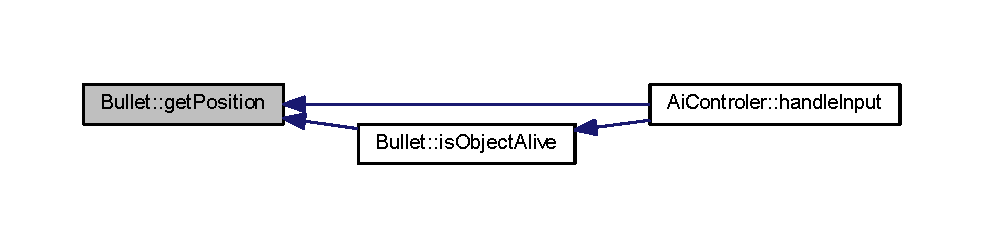
\includegraphics[width=350pt]{class_bullet_a82f82d6367d1c403898a29d1ce91630d_icgraph}
\end{center}
\end{figure}


\hypertarget{class_bullet_a23cadfbb18a562482f0bae03f0edd029}{}\index{Bullet@{Bullet}!is\+Object\+Alive@{is\+Object\+Alive}}
\index{is\+Object\+Alive@{is\+Object\+Alive}!Bullet@{Bullet}}
\subsubsection[{is\+Object\+Alive}]{\setlength{\rightskip}{0pt plus 5cm}bool Bullet\+::is\+Object\+Alive (
\begin{DoxyParamCaption}
\item[{sf\+::\+Render\+Window \&}]{window}
\end{DoxyParamCaption}
)}\label{class_bullet_a23cadfbb18a562482f0bae03f0edd029}


Here is the call graph for this function\+:
\nopagebreak
\begin{figure}[H]
\begin{center}
\leavevmode
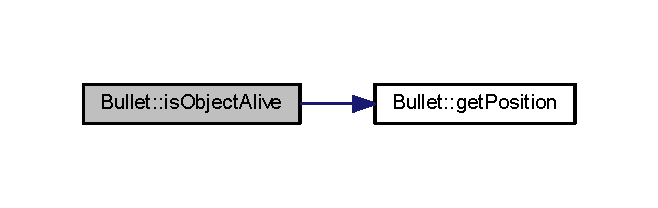
\includegraphics[width=316pt]{class_bullet_a23cadfbb18a562482f0bae03f0edd029_cgraph}
\end{center}
\end{figure}




Here is the caller graph for this function\+:
\nopagebreak
\begin{figure}[H]
\begin{center}
\leavevmode
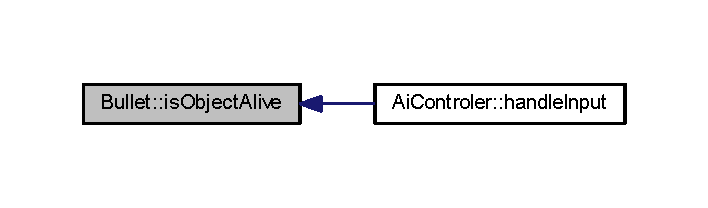
\includegraphics[width=340pt]{class_bullet_a23cadfbb18a562482f0bae03f0edd029_icgraph}
\end{center}
\end{figure}


\hypertarget{class_bullet_a8715ab2edff76c8b45fabc6dc453e85d}{}\index{Bullet@{Bullet}!move@{move}}
\index{move@{move}!Bullet@{Bullet}}
\subsubsection[{move}]{\setlength{\rightskip}{0pt plus 5cm}void Bullet\+::move (
\begin{DoxyParamCaption}
\item[{const sf\+::\+Vector2f \&}]{offset}
\end{DoxyParamCaption}
)\hspace{0.3cm}{\ttfamily [inline]}, {\ttfamily [override]}, {\ttfamily [virtual]}}\label{class_bullet_a8715ab2edff76c8b45fabc6dc453e85d}


Implements \hyperlink{class_game_object_a370e89c4bb00a8fb851d9279480f7f76}{Game\+Object}.

\hypertarget{class_bullet_ae4af350647e1b2a798eb3fd35a883b84}{}\index{Bullet@{Bullet}!render@{render}}
\index{render@{render}!Bullet@{Bullet}}
\subsubsection[{render}]{\setlength{\rightskip}{0pt plus 5cm}void Bullet\+::render (
\begin{DoxyParamCaption}
\item[{sf\+::\+Render\+Window \&}]{window}
\end{DoxyParamCaption}
)\hspace{0.3cm}{\ttfamily [override]}, {\ttfamily [virtual]}}\label{class_bullet_ae4af350647e1b2a798eb3fd35a883b84}


Implements \hyperlink{class_game_object_a07a0da194460f2642732f45d7ad369e8}{Game\+Object}.



The documentation for this class was generated from the following files\+:\begin{DoxyCompactItemize}
\item 
\hyperlink{_bullet_8h}{Bullet.\+h}\item 
\hyperlink{_bullet_8cpp}{Bullet.\+cpp}\end{DoxyCompactItemize}

\hypertarget{class_collision_handler}{}\section{Collision\+Handler Class Reference}
\label{class_collision_handler}\index{Collision\+Handler@{Collision\+Handler}}


{\ttfamily \#include $<$Collision\+Handler.\+h$>$}



Inheritance diagram for Collision\+Handler\+:
\nopagebreak
\begin{figure}[H]
\begin{center}
\leavevmode
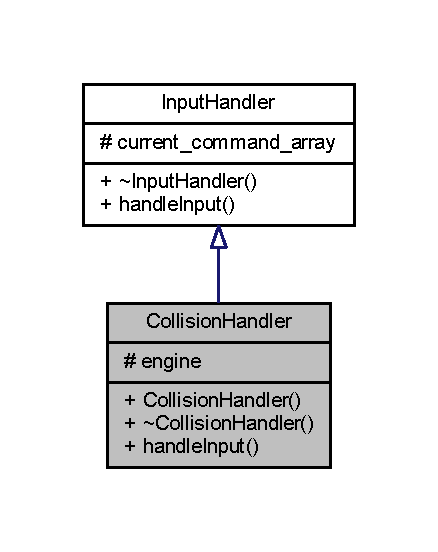
\includegraphics[width=210pt]{class_collision_handler__inherit__graph}
\end{center}
\end{figure}


Collaboration diagram for Collision\+Handler\+:
\nopagebreak
\begin{figure}[H]
\begin{center}
\leavevmode
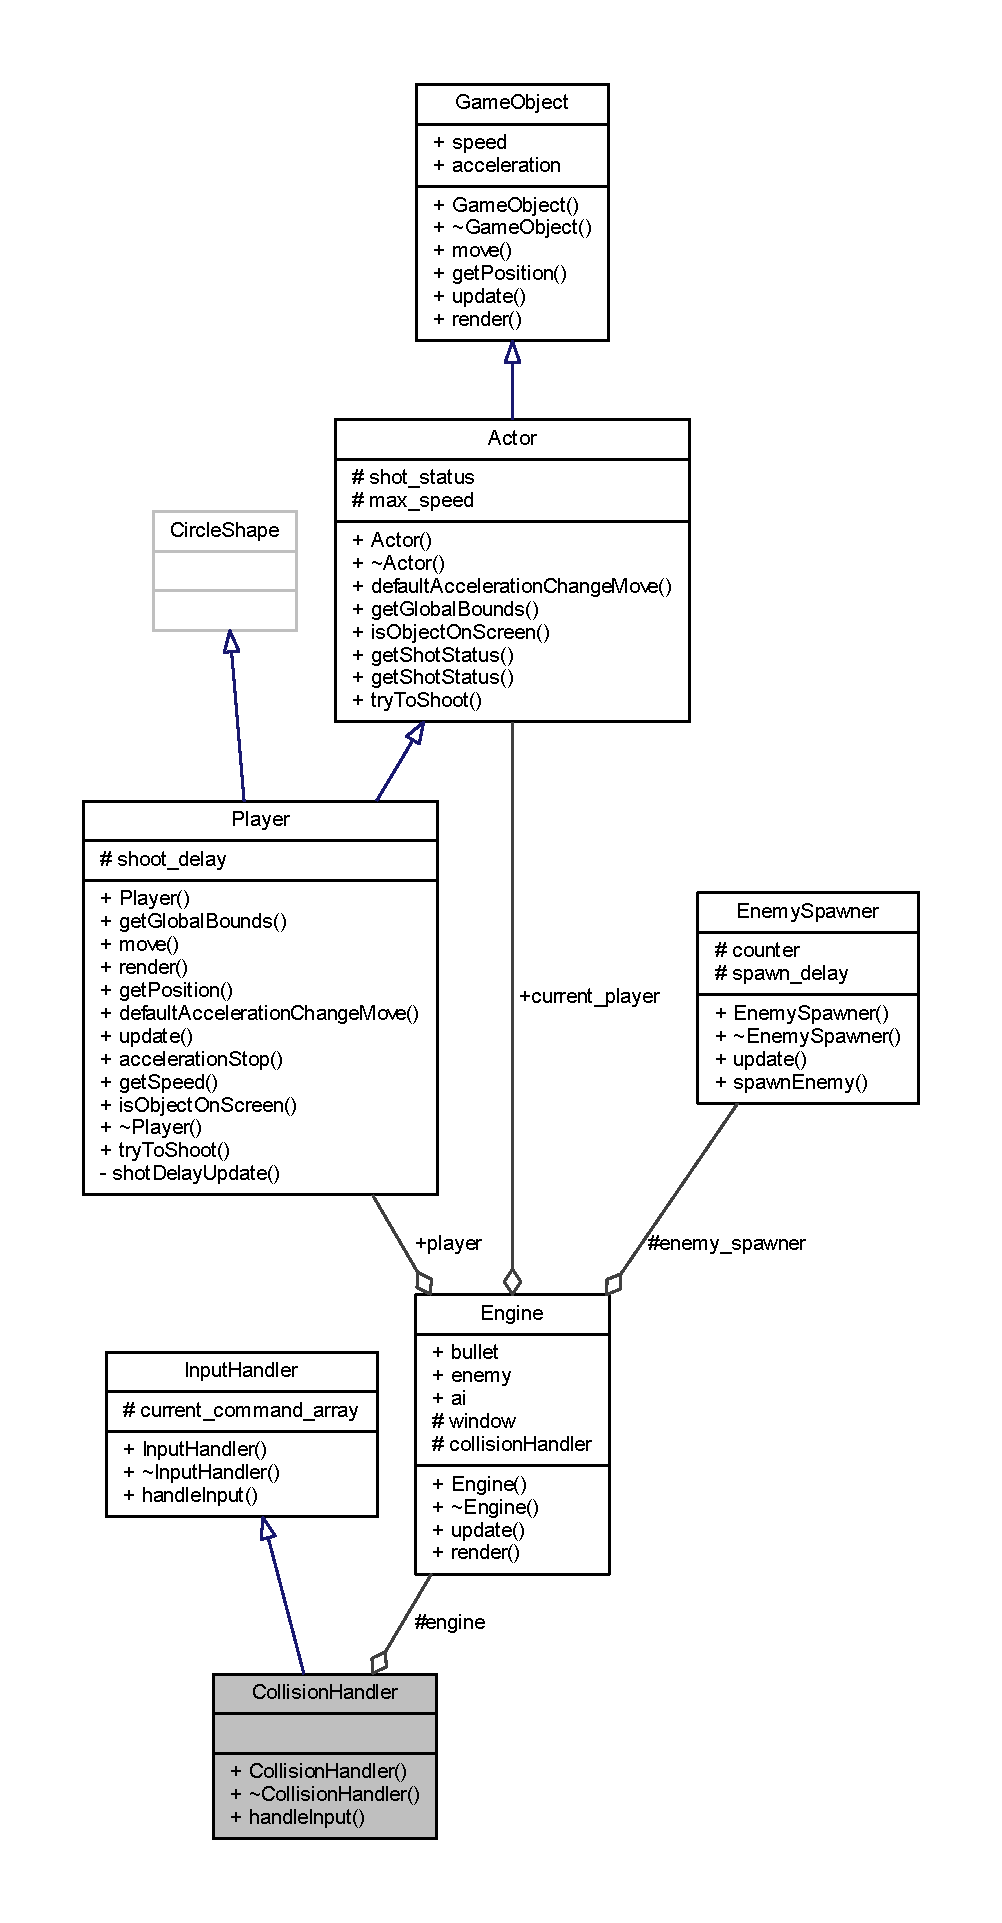
\includegraphics[width=350pt]{class_collision_handler__coll__graph}
\end{center}
\end{figure}
\subsection*{Public Member Functions}
\begin{DoxyCompactItemize}
\item 
\hyperlink{class_collision_handler_a1d575178fc7de4a35e9f0abb1f7f6395}{Collision\+Handler} (\hyperlink{class_engine}{Engine} \&engine\+\_\+in)
\item 
virtual \hyperlink{class_collision_handler_a99f5524cf1706f9ea95500cf273a9d97}{$\sim$\+Collision\+Handler} ()
\item 
\hyperlink{class_command}{Command} $\ast$$\ast$ \hyperlink{class_collision_handler_a7f6deb84dcebcc72e0020eb251ea617f}{handle\+Input} () override
\end{DoxyCompactItemize}
\subsection*{Public Attributes}
\begin{DoxyCompactItemize}
\item 
\hyperlink{class_engine}{Engine} \& \hyperlink{class_collision_handler_ab2f8d7769a6ec8c57814d1eb3a465c6f}{engine}
\end{DoxyCompactItemize}
\subsection*{Additional Inherited Members}


\subsection{Constructor \& Destructor Documentation}
\hypertarget{class_collision_handler_a1d575178fc7de4a35e9f0abb1f7f6395}{}\index{Collision\+Handler@{Collision\+Handler}!Collision\+Handler@{Collision\+Handler}}
\index{Collision\+Handler@{Collision\+Handler}!Collision\+Handler@{Collision\+Handler}}
\subsubsection[{Collision\+Handler}]{\setlength{\rightskip}{0pt plus 5cm}Collision\+Handler\+::\+Collision\+Handler (
\begin{DoxyParamCaption}
\item[{{\bf Engine} \&}]{engine\+\_\+in}
\end{DoxyParamCaption}
)}\label{class_collision_handler_a1d575178fc7de4a35e9f0abb1f7f6395}
\hypertarget{class_collision_handler_a99f5524cf1706f9ea95500cf273a9d97}{}\index{Collision\+Handler@{Collision\+Handler}!````~Collision\+Handler@{$\sim$\+Collision\+Handler}}
\index{````~Collision\+Handler@{$\sim$\+Collision\+Handler}!Collision\+Handler@{Collision\+Handler}}
\subsubsection[{$\sim$\+Collision\+Handler}]{\setlength{\rightskip}{0pt plus 5cm}Collision\+Handler\+::$\sim$\+Collision\+Handler (
\begin{DoxyParamCaption}
{}
\end{DoxyParamCaption}
)\hspace{0.3cm}{\ttfamily [virtual]}}\label{class_collision_handler_a99f5524cf1706f9ea95500cf273a9d97}


\subsection{Member Function Documentation}
\hypertarget{class_collision_handler_a7f6deb84dcebcc72e0020eb251ea617f}{}\index{Collision\+Handler@{Collision\+Handler}!handle\+Input@{handle\+Input}}
\index{handle\+Input@{handle\+Input}!Collision\+Handler@{Collision\+Handler}}
\subsubsection[{handle\+Input}]{\setlength{\rightskip}{0pt plus 5cm}{\bf Command} $\ast$$\ast$ Collision\+Handler\+::handle\+Input (
\begin{DoxyParamCaption}
{}
\end{DoxyParamCaption}
)\hspace{0.3cm}{\ttfamily [override]}, {\ttfamily [virtual]}}\label{class_collision_handler_a7f6deb84dcebcc72e0020eb251ea617f}


Implements \hyperlink{class_input_handler_a69b726d4a409a6f4ae443689cb69b404}{Input\+Handler}.



\subsection{Member Data Documentation}
\hypertarget{class_collision_handler_ab2f8d7769a6ec8c57814d1eb3a465c6f}{}\index{Collision\+Handler@{Collision\+Handler}!engine@{engine}}
\index{engine@{engine}!Collision\+Handler@{Collision\+Handler}}
\subsubsection[{engine}]{\setlength{\rightskip}{0pt plus 5cm}{\bf Engine}\& Collision\+Handler\+::engine}\label{class_collision_handler_ab2f8d7769a6ec8c57814d1eb3a465c6f}


The documentation for this class was generated from the following files\+:\begin{DoxyCompactItemize}
\item 
\hyperlink{_collision_handler_8h}{Collision\+Handler.\+h}\item 
\hyperlink{_collision_handler_8cpp}{Collision\+Handler.\+cpp}\end{DoxyCompactItemize}

\hypertarget{class_command}{}\section{Command Class Reference}
\label{class_command}\index{Command@{Command}}


{\ttfamily \#include $<$Command.\+h$>$}



Inheritance diagram for Command\+:
\nopagebreak
\begin{figure}[H]
\begin{center}
\leavevmode
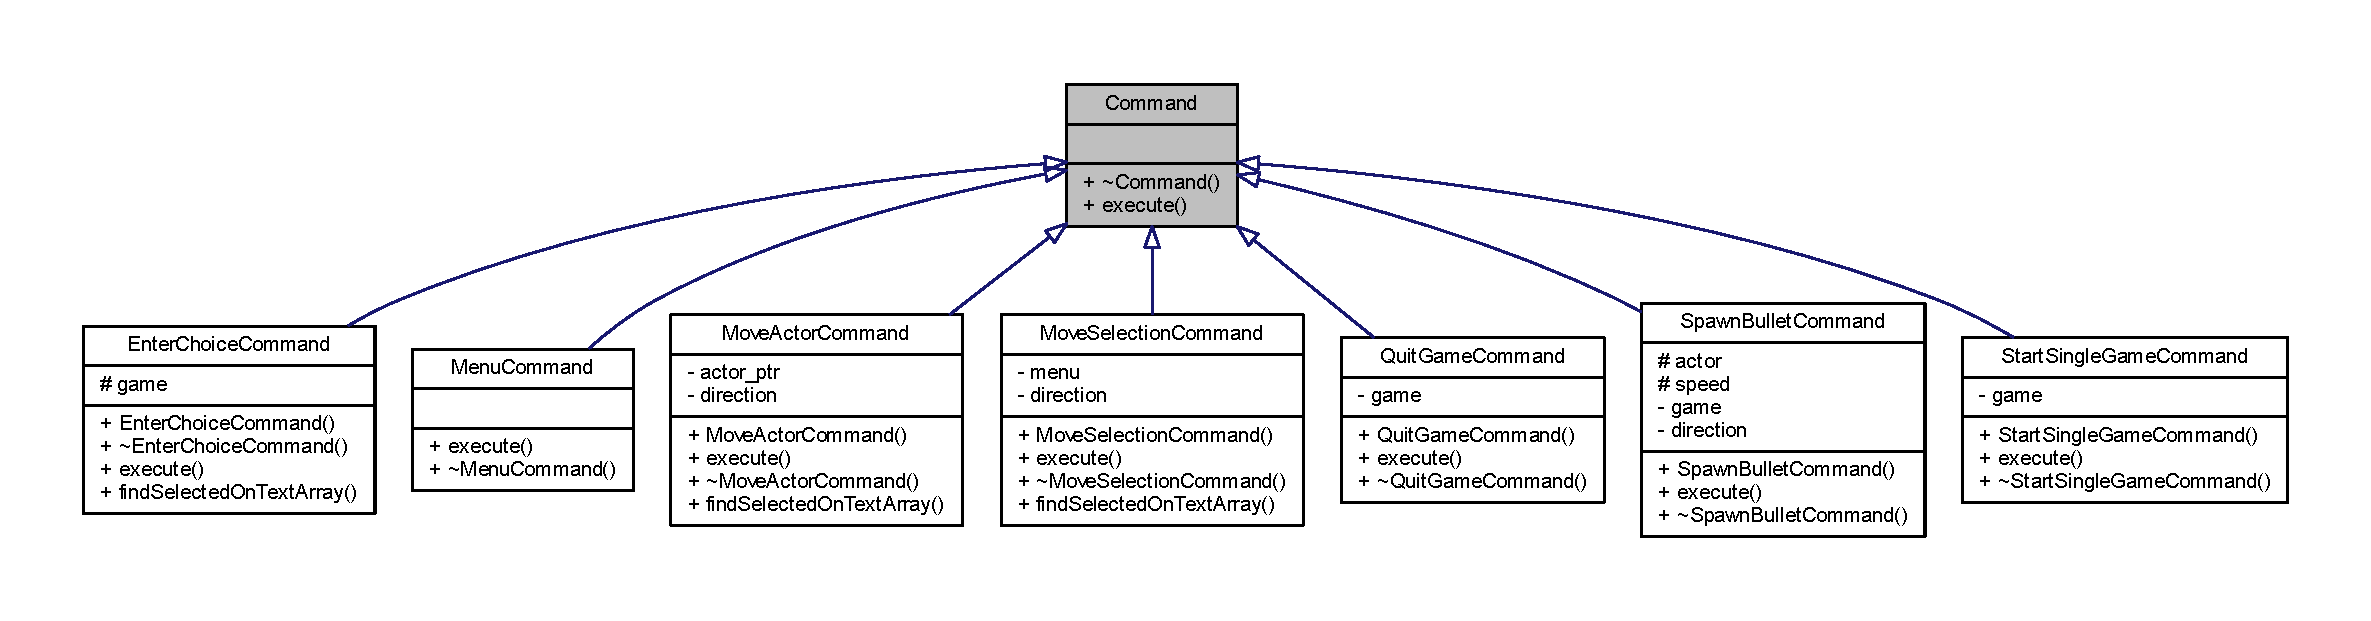
\includegraphics[width=350pt]{class_command__inherit__graph}
\end{center}
\end{figure}


Collaboration diagram for Command\+:\nopagebreak
\begin{figure}[H]
\begin{center}
\leavevmode
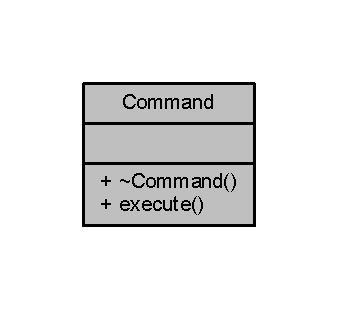
\includegraphics[width=162pt]{class_command__coll__graph}
\end{center}
\end{figure}
\subsection*{Public Member Functions}
\begin{DoxyCompactItemize}
\item 
virtual \hyperlink{class_command_ab552bb3a07fdd1acbfd8ea76e69b2278}{$\sim$\+Command} ()
\item 
virtual void \hyperlink{class_command_a6fd7d9bd8df8bfc881e4d6c7cd1878b7}{execute} ()=0
\end{DoxyCompactItemize}


\subsection{Constructor \& Destructor Documentation}
\hypertarget{class_command_ab552bb3a07fdd1acbfd8ea76e69b2278}{}\index{Command@{Command}!````~Command@{$\sim$\+Command}}
\index{````~Command@{$\sim$\+Command}!Command@{Command}}
\subsubsection[{$\sim$\+Command}]{\setlength{\rightskip}{0pt plus 5cm}Command\+::$\sim$\+Command (
\begin{DoxyParamCaption}
{}
\end{DoxyParamCaption}
)\hspace{0.3cm}{\ttfamily [virtual]}}\label{class_command_ab552bb3a07fdd1acbfd8ea76e69b2278}


\subsection{Member Function Documentation}
\hypertarget{class_command_a6fd7d9bd8df8bfc881e4d6c7cd1878b7}{}\index{Command@{Command}!execute@{execute}}
\index{execute@{execute}!Command@{Command}}
\subsubsection[{execute}]{\setlength{\rightskip}{0pt plus 5cm}virtual void Command\+::execute (
\begin{DoxyParamCaption}
{}
\end{DoxyParamCaption}
)\hspace{0.3cm}{\ttfamily [pure virtual]}}\label{class_command_a6fd7d9bd8df8bfc881e4d6c7cd1878b7}


Implemented in \hyperlink{class_enter_choice_command_a684f65bfc296353ecefc6edc1c678c70}{Enter\+Choice\+Command}, \hyperlink{class_move_actor_command_a62ff2dc8808da57913d1e5aa43c10cfb}{Move\+Actor\+Command}, \hyperlink{class_spawn_bullet_command_a558af584b91637cd6bcf989d799eca4d}{Spawn\+Bullet\+Command}, \hyperlink{class_start_single_game_command_a27e779a9ce1664557266c0e7679faab0}{Start\+Single\+Game\+Command}, \hyperlink{class_move_selection_command_a0d2117e50adfe980744b3ca883ca7fc5}{Move\+Selection\+Command}, \hyperlink{class_menu_command_ac5d1ade9cec6d0540cb8e9ff0e84574c}{Menu\+Command}, and \hyperlink{class_quit_game_command_ad39d43150a927d7e8b0dd7162eb840eb}{Quit\+Game\+Command}.



The documentation for this class was generated from the following files\+:\begin{DoxyCompactItemize}
\item 
\hyperlink{_command_8h}{Command.\+h}\item 
\hyperlink{_command_8cpp}{Command.\+cpp}\end{DoxyCompactItemize}

\hypertarget{class_enemy}{}\section{Enemy Class Reference}
\label{class_enemy}\index{Enemy@{Enemy}}


{\ttfamily \#include $<$Enemy.\+h$>$}



Inheritance diagram for Enemy\+:
\nopagebreak
\begin{figure}[H]
\begin{center}
\leavevmode
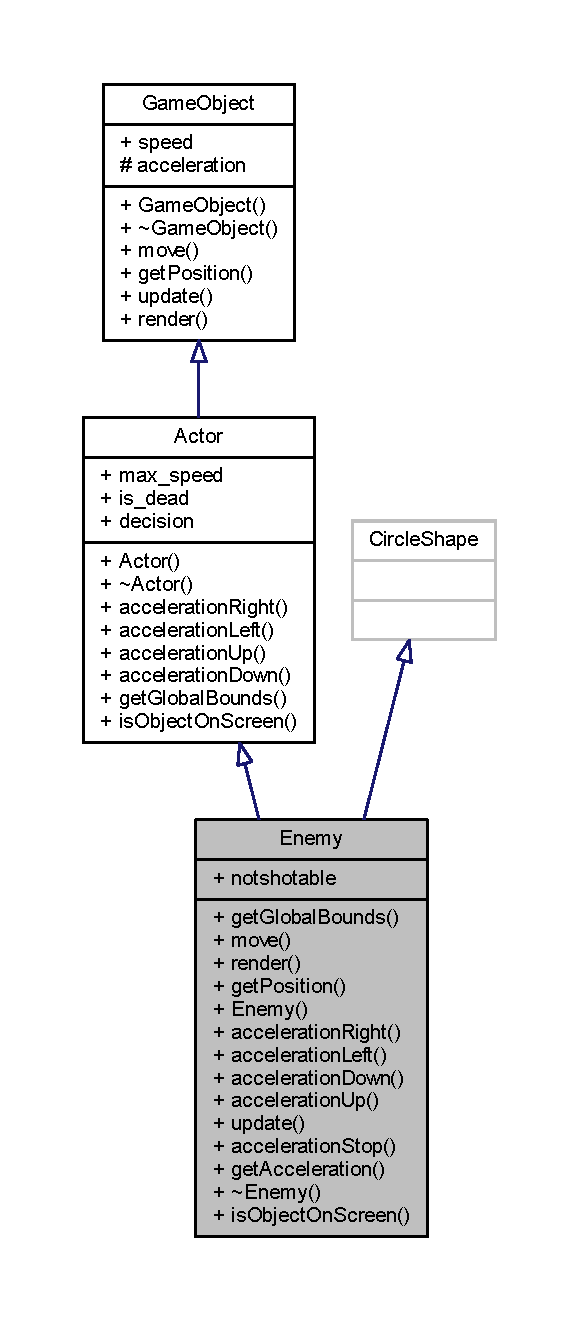
\includegraphics[height=550pt]{class_enemy__inherit__graph}
\end{center}
\end{figure}


Collaboration diagram for Enemy\+:
\nopagebreak
\begin{figure}[H]
\begin{center}
\leavevmode
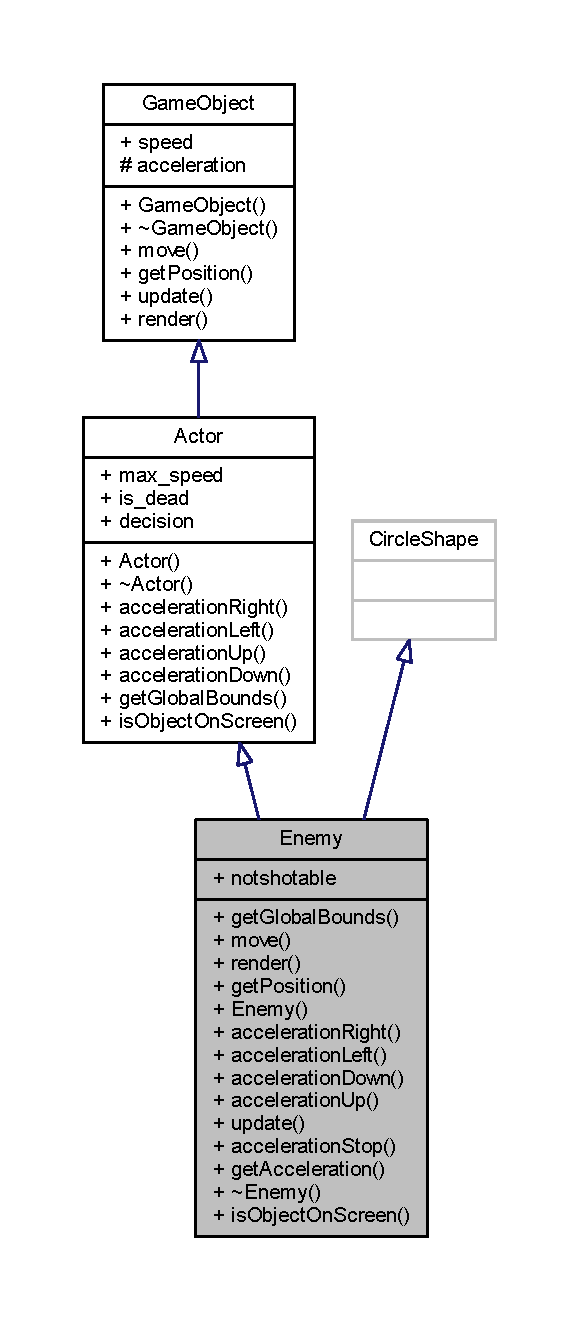
\includegraphics[height=550pt]{class_enemy__coll__graph}
\end{center}
\end{figure}
\subsection*{Public Member Functions}
\begin{DoxyCompactItemize}
\item 
virtual sf\+::\+Float\+Rect \hyperlink{class_enemy_abb50439b9517d5a2b4c6b6c6a4e91672}{get\+Global\+Bounds} () override
\item 
virtual void \hyperlink{class_enemy_a4db256c45aa8d835561e035969883069}{move} (const sf\+::\+Vector2f \&offset)
\item 
virtual void \hyperlink{class_enemy_a409d7d48e2f6bb27f878691f14a79957}{render} (sf\+::\+Render\+Window \&window)
\item 
const sf\+::\+Vector2f \& \hyperlink{class_enemy_ade0ec5d0a52a35a387a4cdcccf4c9ddc}{get\+Position} () const override
\item 
\hyperlink{class_enemy_a94f30d348b6d2840fd71675472ba38dd}{Enemy} ()
\item 
void \hyperlink{class_enemy_ae642ab230b9b416142cfe2a6ed3e3aeb}{default\+Acceleration\+Change\+Move} (\hyperlink{namespace_general_tools_afedc3bd242369903830dec92c3ad569b}{General\+Tools\+::\+Direction} direction)
\item 
void \hyperlink{class_enemy_a842ae08ff3a191b3bfd5a0f865b968be}{acceleration\+Left} ()
\item 
void \hyperlink{class_enemy_a901af192d36d757b0cfbd2c92c742ccc}{acceleration\+Down} ()
\item 
void \hyperlink{class_enemy_acb3226b1c27efc097b3817a8efde1e93}{acceleration\+Up} ()
\item 
void \hyperlink{class_enemy_aa70d742da02995011f1618acc9e303db}{update} () override
\item 
sf\+::\+Vector2f \hyperlink{class_enemy_a8c53ca8541fdfc43b8464feeabefc150}{get\+Speed} ()
\item 
virtual \hyperlink{class_enemy_ac0eec4755e28c02688065f9657150ac3}{$\sim$\+Enemy} ()
\item 
bool \hyperlink{class_enemy_a9a6b7416616b3d0464978d38cf7095e9}{is\+Object\+On\+Screen} (sf\+::\+Render\+Window \&window) override
\end{DoxyCompactItemize}
\subsection*{Additional Inherited Members}


\subsection{Constructor \& Destructor Documentation}
\hypertarget{class_enemy_a94f30d348b6d2840fd71675472ba38dd}{}\index{Enemy@{Enemy}!Enemy@{Enemy}}
\index{Enemy@{Enemy}!Enemy@{Enemy}}
\subsubsection[{Enemy}]{\setlength{\rightskip}{0pt plus 5cm}Enemy\+::\+Enemy (
\begin{DoxyParamCaption}
{}
\end{DoxyParamCaption}
)}\label{class_enemy_a94f30d348b6d2840fd71675472ba38dd}


Here is the call graph for this function\+:\nopagebreak
\begin{figure}[H]
\begin{center}
\leavevmode
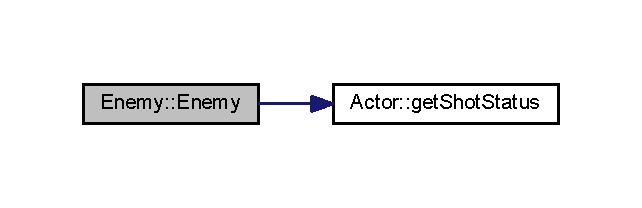
\includegraphics[width=308pt]{class_enemy_a94f30d348b6d2840fd71675472ba38dd_cgraph}
\end{center}
\end{figure}


\hypertarget{class_enemy_ac0eec4755e28c02688065f9657150ac3}{}\index{Enemy@{Enemy}!````~Enemy@{$\sim$\+Enemy}}
\index{````~Enemy@{$\sim$\+Enemy}!Enemy@{Enemy}}
\subsubsection[{$\sim$\+Enemy}]{\setlength{\rightskip}{0pt plus 5cm}Enemy\+::$\sim$\+Enemy (
\begin{DoxyParamCaption}
{}
\end{DoxyParamCaption}
)\hspace{0.3cm}{\ttfamily [virtual]}}\label{class_enemy_ac0eec4755e28c02688065f9657150ac3}


\subsection{Member Function Documentation}
\hypertarget{class_enemy_a901af192d36d757b0cfbd2c92c742ccc}{}\index{Enemy@{Enemy}!acceleration\+Down@{acceleration\+Down}}
\index{acceleration\+Down@{acceleration\+Down}!Enemy@{Enemy}}
\subsubsection[{acceleration\+Down}]{\setlength{\rightskip}{0pt plus 5cm}void Enemy\+::acceleration\+Down (
\begin{DoxyParamCaption}
{}
\end{DoxyParamCaption}
)}\label{class_enemy_a901af192d36d757b0cfbd2c92c742ccc}


Here is the caller graph for this function\+:\nopagebreak
\begin{figure}[H]
\begin{center}
\leavevmode
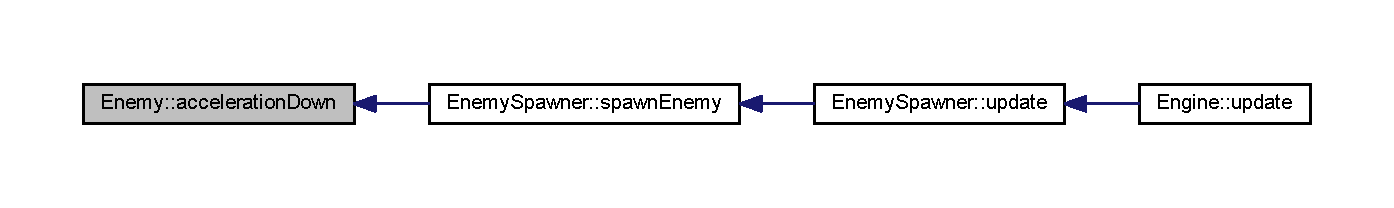
\includegraphics[width=350pt]{class_enemy_a901af192d36d757b0cfbd2c92c742ccc_icgraph}
\end{center}
\end{figure}


\hypertarget{class_enemy_a842ae08ff3a191b3bfd5a0f865b968be}{}\index{Enemy@{Enemy}!acceleration\+Left@{acceleration\+Left}}
\index{acceleration\+Left@{acceleration\+Left}!Enemy@{Enemy}}
\subsubsection[{acceleration\+Left}]{\setlength{\rightskip}{0pt plus 5cm}void Enemy\+::acceleration\+Left (
\begin{DoxyParamCaption}
{}
\end{DoxyParamCaption}
)}\label{class_enemy_a842ae08ff3a191b3bfd5a0f865b968be}
\hypertarget{class_enemy_acb3226b1c27efc097b3817a8efde1e93}{}\index{Enemy@{Enemy}!acceleration\+Up@{acceleration\+Up}}
\index{acceleration\+Up@{acceleration\+Up}!Enemy@{Enemy}}
\subsubsection[{acceleration\+Up}]{\setlength{\rightskip}{0pt plus 5cm}void Enemy\+::acceleration\+Up (
\begin{DoxyParamCaption}
{}
\end{DoxyParamCaption}
)}\label{class_enemy_acb3226b1c27efc097b3817a8efde1e93}
\hypertarget{class_enemy_ae642ab230b9b416142cfe2a6ed3e3aeb}{}\index{Enemy@{Enemy}!default\+Acceleration\+Change\+Move@{default\+Acceleration\+Change\+Move}}
\index{default\+Acceleration\+Change\+Move@{default\+Acceleration\+Change\+Move}!Enemy@{Enemy}}
\subsubsection[{default\+Acceleration\+Change\+Move}]{\setlength{\rightskip}{0pt plus 5cm}void Enemy\+::default\+Acceleration\+Change\+Move (
\begin{DoxyParamCaption}
\item[{{\bf General\+Tools\+::\+Direction}}]{direction}
\end{DoxyParamCaption}
)\hspace{0.3cm}{\ttfamily [virtual]}}\label{class_enemy_ae642ab230b9b416142cfe2a6ed3e3aeb}


Implements \hyperlink{class_actor_a9992ceb5499bff601e461c3bb93a8d48}{Actor}.

\hypertarget{class_enemy_abb50439b9517d5a2b4c6b6c6a4e91672}{}\index{Enemy@{Enemy}!get\+Global\+Bounds@{get\+Global\+Bounds}}
\index{get\+Global\+Bounds@{get\+Global\+Bounds}!Enemy@{Enemy}}
\subsubsection[{get\+Global\+Bounds}]{\setlength{\rightskip}{0pt plus 5cm}virtual sf\+::\+Float\+Rect Enemy\+::get\+Global\+Bounds (
\begin{DoxyParamCaption}
{}
\end{DoxyParamCaption}
)\hspace{0.3cm}{\ttfamily [inline]}, {\ttfamily [override]}, {\ttfamily [virtual]}}\label{class_enemy_abb50439b9517d5a2b4c6b6c6a4e91672}


Implements \hyperlink{class_actor_ab56cff32076fef8392f4562fe281ea86}{Actor}.



Here is the caller graph for this function\+:\nopagebreak
\begin{figure}[H]
\begin{center}
\leavevmode
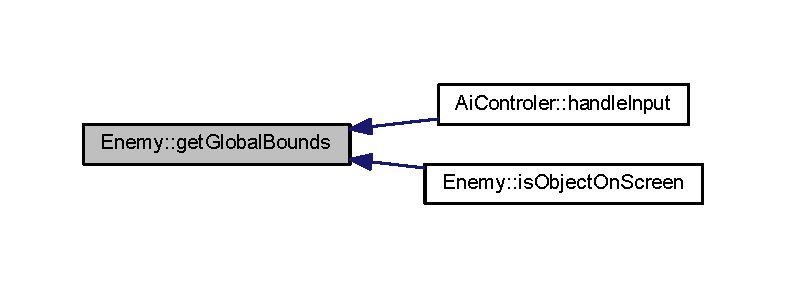
\includegraphics[width=350pt]{class_enemy_abb50439b9517d5a2b4c6b6c6a4e91672_icgraph}
\end{center}
\end{figure}


\hypertarget{class_enemy_ade0ec5d0a52a35a387a4cdcccf4c9ddc}{}\index{Enemy@{Enemy}!get\+Position@{get\+Position}}
\index{get\+Position@{get\+Position}!Enemy@{Enemy}}
\subsubsection[{get\+Position}]{\setlength{\rightskip}{0pt plus 5cm}const sf\+::\+Vector2f \& Enemy\+::get\+Position (
\begin{DoxyParamCaption}
{}
\end{DoxyParamCaption}
) const\hspace{0.3cm}{\ttfamily [override]}, {\ttfamily [virtual]}}\label{class_enemy_ade0ec5d0a52a35a387a4cdcccf4c9ddc}


Implements \hyperlink{class_game_object_aba7c07744a79defec4484fb09d917543}{Game\+Object}.



Here is the caller graph for this function\+:\nopagebreak
\begin{figure}[H]
\begin{center}
\leavevmode
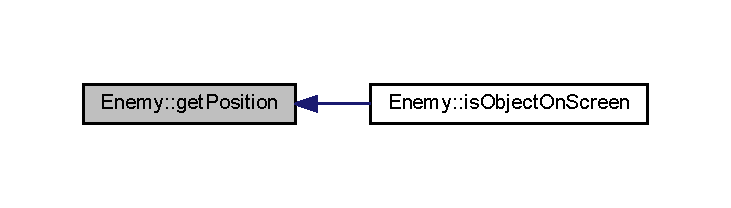
\includegraphics[width=350pt]{class_enemy_ade0ec5d0a52a35a387a4cdcccf4c9ddc_icgraph}
\end{center}
\end{figure}


\hypertarget{class_enemy_a8c53ca8541fdfc43b8464feeabefc150}{}\index{Enemy@{Enemy}!get\+Speed@{get\+Speed}}
\index{get\+Speed@{get\+Speed}!Enemy@{Enemy}}
\subsubsection[{get\+Speed}]{\setlength{\rightskip}{0pt plus 5cm}sf\+::\+Vector2f Enemy\+::get\+Speed (
\begin{DoxyParamCaption}
{}
\end{DoxyParamCaption}
)\hspace{0.3cm}{\ttfamily [inline]}}\label{class_enemy_a8c53ca8541fdfc43b8464feeabefc150}
\hypertarget{class_enemy_a9a6b7416616b3d0464978d38cf7095e9}{}\index{Enemy@{Enemy}!is\+Object\+On\+Screen@{is\+Object\+On\+Screen}}
\index{is\+Object\+On\+Screen@{is\+Object\+On\+Screen}!Enemy@{Enemy}}
\subsubsection[{is\+Object\+On\+Screen}]{\setlength{\rightskip}{0pt plus 5cm}bool Enemy\+::is\+Object\+On\+Screen (
\begin{DoxyParamCaption}
\item[{sf\+::\+Render\+Window \&}]{window}
\end{DoxyParamCaption}
)\hspace{0.3cm}{\ttfamily [override]}, {\ttfamily [virtual]}}\label{class_enemy_a9a6b7416616b3d0464978d38cf7095e9}


Implements \hyperlink{class_actor_a0bd104ef42ef1e3c3eea5c58e94c2429}{Actor}.



Here is the call graph for this function\+:\nopagebreak
\begin{figure}[H]
\begin{center}
\leavevmode
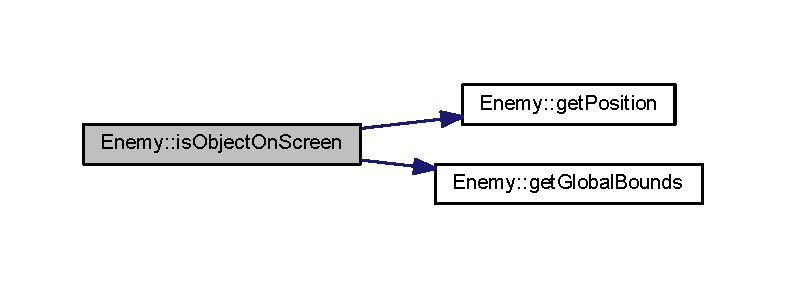
\includegraphics[width=350pt]{class_enemy_a9a6b7416616b3d0464978d38cf7095e9_cgraph}
\end{center}
\end{figure}


\hypertarget{class_enemy_a4db256c45aa8d835561e035969883069}{}\index{Enemy@{Enemy}!move@{move}}
\index{move@{move}!Enemy@{Enemy}}
\subsubsection[{move}]{\setlength{\rightskip}{0pt plus 5cm}virtual void Enemy\+::move (
\begin{DoxyParamCaption}
\item[{const sf\+::\+Vector2f \&}]{offset}
\end{DoxyParamCaption}
)\hspace{0.3cm}{\ttfamily [inline]}, {\ttfamily [virtual]}}\label{class_enemy_a4db256c45aa8d835561e035969883069}


Implements \hyperlink{class_game_object_a370e89c4bb00a8fb851d9279480f7f76}{Game\+Object}.



Here is the caller graph for this function\+:\nopagebreak
\begin{figure}[H]
\begin{center}
\leavevmode
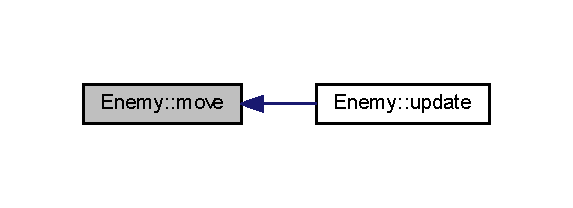
\includegraphics[width=275pt]{class_enemy_a4db256c45aa8d835561e035969883069_icgraph}
\end{center}
\end{figure}


\hypertarget{class_enemy_a409d7d48e2f6bb27f878691f14a79957}{}\index{Enemy@{Enemy}!render@{render}}
\index{render@{render}!Enemy@{Enemy}}
\subsubsection[{render}]{\setlength{\rightskip}{0pt plus 5cm}virtual void Enemy\+::render (
\begin{DoxyParamCaption}
\item[{sf\+::\+Render\+Window \&}]{window}
\end{DoxyParamCaption}
)\hspace{0.3cm}{\ttfamily [inline]}, {\ttfamily [virtual]}}\label{class_enemy_a409d7d48e2f6bb27f878691f14a79957}


Implements \hyperlink{class_game_object_a07a0da194460f2642732f45d7ad369e8}{Game\+Object}.

\hypertarget{class_enemy_aa70d742da02995011f1618acc9e303db}{}\index{Enemy@{Enemy}!update@{update}}
\index{update@{update}!Enemy@{Enemy}}
\subsubsection[{update}]{\setlength{\rightskip}{0pt plus 5cm}void Enemy\+::update (
\begin{DoxyParamCaption}
{}
\end{DoxyParamCaption}
)\hspace{0.3cm}{\ttfamily [override]}, {\ttfamily [virtual]}}\label{class_enemy_aa70d742da02995011f1618acc9e303db}


Reimplemented from \hyperlink{class_game_object_ad4a07f19f6c5e2e71c89c07486f26244}{Game\+Object}.



Here is the call graph for this function\+:\nopagebreak
\begin{figure}[H]
\begin{center}
\leavevmode
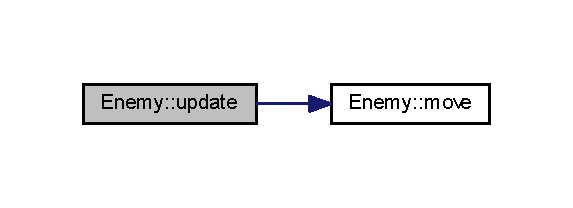
\includegraphics[width=275pt]{class_enemy_aa70d742da02995011f1618acc9e303db_cgraph}
\end{center}
\end{figure}




The documentation for this class was generated from the following files\+:\begin{DoxyCompactItemize}
\item 
\hyperlink{_enemy_8h}{Enemy.\+h}\item 
\hyperlink{_enemy_8cpp}{Enemy.\+cpp}\end{DoxyCompactItemize}

\hypertarget{class_enemy_spawner}{}\section{Enemy\+Spawner Class Reference}
\label{class_enemy_spawner}\index{Enemy\+Spawner@{Enemy\+Spawner}}


{\ttfamily \#include $<$Enemy\+Spawner.\+h$>$}



Collaboration diagram for Enemy\+Spawner\+:
\nopagebreak
\begin{figure}[H]
\begin{center}
\leavevmode
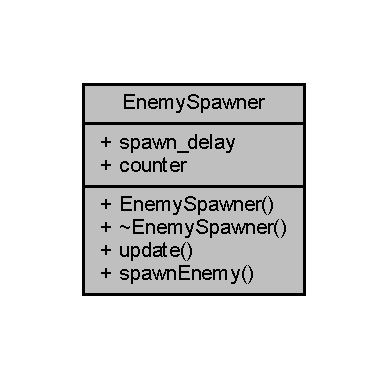
\includegraphics[width=186pt]{class_enemy_spawner__coll__graph}
\end{center}
\end{figure}
\subsection*{Public Member Functions}
\begin{DoxyCompactItemize}
\item 
\hyperlink{class_enemy_spawner_a4c3dac46ddd4f9e97bac15cf42b2f931}{Enemy\+Spawner} ()
\item 
virtual \hyperlink{class_enemy_spawner_a661639d8aa3e52a1249883c34d11f0ad}{$\sim$\+Enemy\+Spawner} ()
\item 
\hyperlink{class_enemy}{Enemy} $\ast$ \hyperlink{class_enemy_spawner_a1b00731679380c088027072b11583d6c}{update} ()
\item 
\hyperlink{class_enemy}{Enemy} $\ast$ \hyperlink{class_enemy_spawner_adc9ba92ad7028dc28e1599fea871e132}{spawn\+Enemy} ()
\end{DoxyCompactItemize}
\subsection*{Protected Attributes}
\begin{DoxyCompactItemize}
\item 
int \hyperlink{class_enemy_spawner_a10072a5aab9a1d055df222ee0ef3fe6e}{counter}
\item 
const int \hyperlink{class_enemy_spawner_a925cbf3cbaadaf7b376ef6aadc955d7f}{spawn\+\_\+delay}
\end{DoxyCompactItemize}


\subsection{Constructor \& Destructor Documentation}
\hypertarget{class_enemy_spawner_a4c3dac46ddd4f9e97bac15cf42b2f931}{}\index{Enemy\+Spawner@{Enemy\+Spawner}!Enemy\+Spawner@{Enemy\+Spawner}}
\index{Enemy\+Spawner@{Enemy\+Spawner}!Enemy\+Spawner@{Enemy\+Spawner}}
\subsubsection[{Enemy\+Spawner}]{\setlength{\rightskip}{0pt plus 5cm}Enemy\+Spawner\+::\+Enemy\+Spawner (
\begin{DoxyParamCaption}
{}
\end{DoxyParamCaption}
)}\label{class_enemy_spawner_a4c3dac46ddd4f9e97bac15cf42b2f931}
\hypertarget{class_enemy_spawner_a661639d8aa3e52a1249883c34d11f0ad}{}\index{Enemy\+Spawner@{Enemy\+Spawner}!````~Enemy\+Spawner@{$\sim$\+Enemy\+Spawner}}
\index{````~Enemy\+Spawner@{$\sim$\+Enemy\+Spawner}!Enemy\+Spawner@{Enemy\+Spawner}}
\subsubsection[{$\sim$\+Enemy\+Spawner}]{\setlength{\rightskip}{0pt plus 5cm}Enemy\+Spawner\+::$\sim$\+Enemy\+Spawner (
\begin{DoxyParamCaption}
{}
\end{DoxyParamCaption}
)\hspace{0.3cm}{\ttfamily [virtual]}}\label{class_enemy_spawner_a661639d8aa3e52a1249883c34d11f0ad}


\subsection{Member Function Documentation}
\hypertarget{class_enemy_spawner_adc9ba92ad7028dc28e1599fea871e132}{}\index{Enemy\+Spawner@{Enemy\+Spawner}!spawn\+Enemy@{spawn\+Enemy}}
\index{spawn\+Enemy@{spawn\+Enemy}!Enemy\+Spawner@{Enemy\+Spawner}}
\subsubsection[{spawn\+Enemy}]{\setlength{\rightskip}{0pt plus 5cm}{\bf Enemy} $\ast$ Enemy\+Spawner\+::spawn\+Enemy (
\begin{DoxyParamCaption}
{}
\end{DoxyParamCaption}
)}\label{class_enemy_spawner_adc9ba92ad7028dc28e1599fea871e132}


Here is the call graph for this function\+:\nopagebreak
\begin{figure}[H]
\begin{center}
\leavevmode
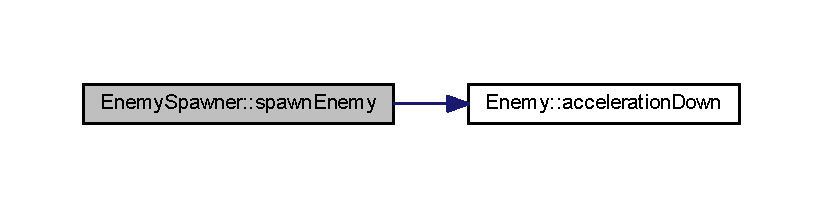
\includegraphics[width=350pt]{class_enemy_spawner_adc9ba92ad7028dc28e1599fea871e132_cgraph}
\end{center}
\end{figure}




Here is the caller graph for this function\+:\nopagebreak
\begin{figure}[H]
\begin{center}
\leavevmode
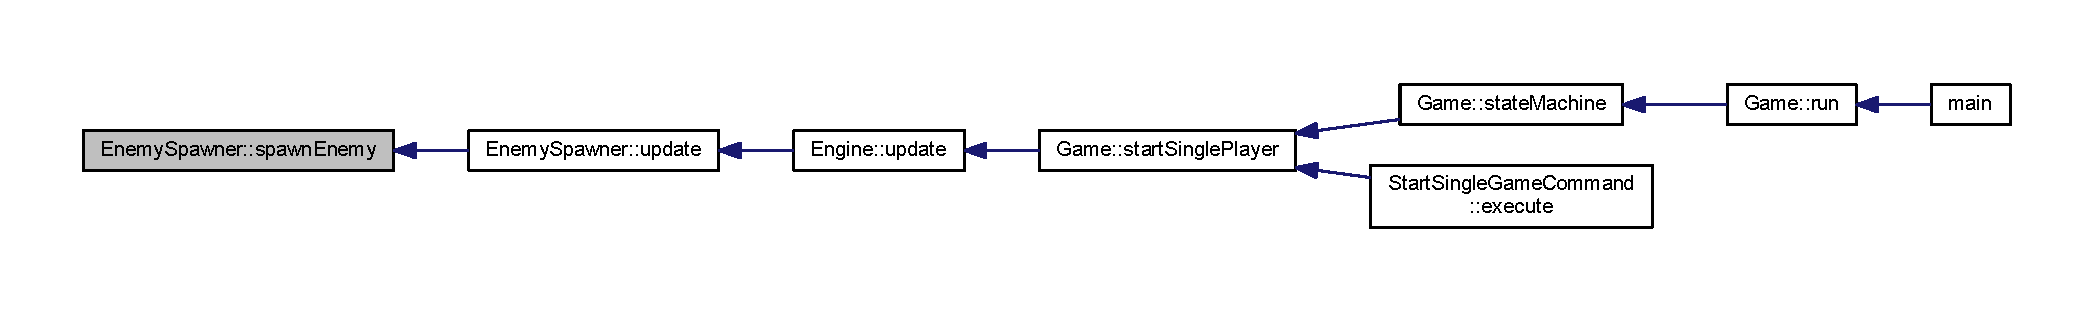
\includegraphics[width=350pt]{class_enemy_spawner_adc9ba92ad7028dc28e1599fea871e132_icgraph}
\end{center}
\end{figure}


\hypertarget{class_enemy_spawner_a1b00731679380c088027072b11583d6c}{}\index{Enemy\+Spawner@{Enemy\+Spawner}!update@{update}}
\index{update@{update}!Enemy\+Spawner@{Enemy\+Spawner}}
\subsubsection[{update}]{\setlength{\rightskip}{0pt plus 5cm}{\bf Enemy} $\ast$ Enemy\+Spawner\+::update (
\begin{DoxyParamCaption}
{}
\end{DoxyParamCaption}
)}\label{class_enemy_spawner_a1b00731679380c088027072b11583d6c}


Here is the call graph for this function\+:\nopagebreak
\begin{figure}[H]
\begin{center}
\leavevmode
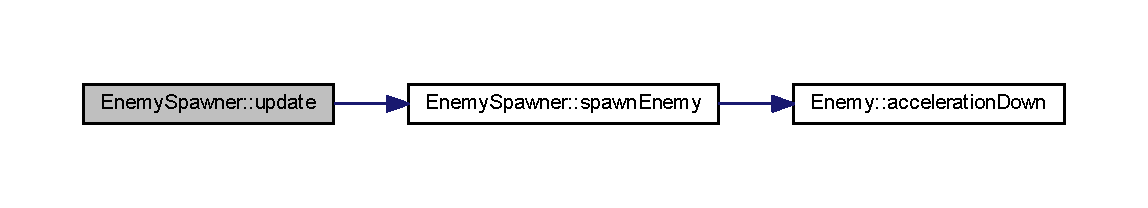
\includegraphics[width=350pt]{class_enemy_spawner_a1b00731679380c088027072b11583d6c_cgraph}
\end{center}
\end{figure}




Here is the caller graph for this function\+:\nopagebreak
\begin{figure}[H]
\begin{center}
\leavevmode
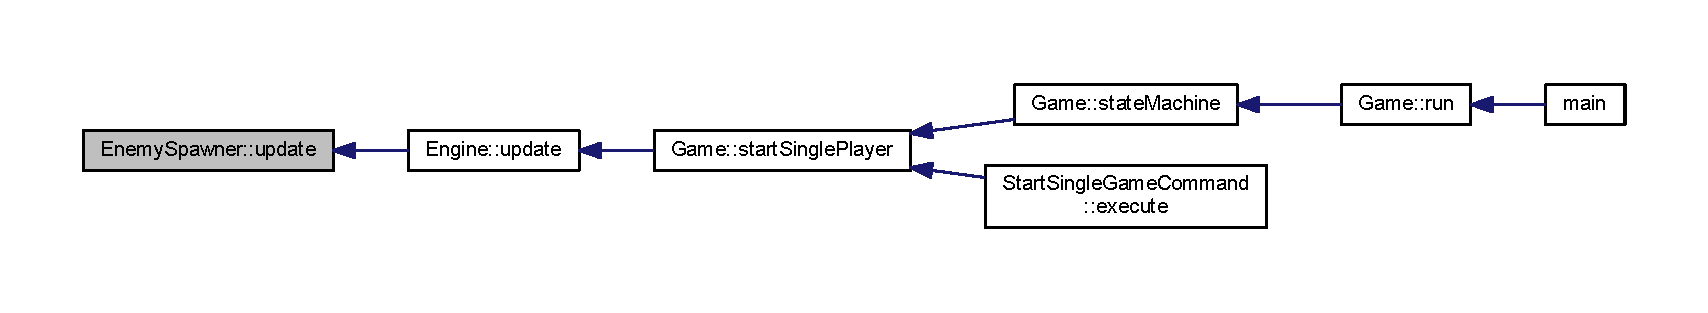
\includegraphics[width=318pt]{class_enemy_spawner_a1b00731679380c088027072b11583d6c_icgraph}
\end{center}
\end{figure}




\subsection{Member Data Documentation}
\hypertarget{class_enemy_spawner_a10072a5aab9a1d055df222ee0ef3fe6e}{}\index{Enemy\+Spawner@{Enemy\+Spawner}!counter@{counter}}
\index{counter@{counter}!Enemy\+Spawner@{Enemy\+Spawner}}
\subsubsection[{counter}]{\setlength{\rightskip}{0pt plus 5cm}int Enemy\+Spawner\+::counter\hspace{0.3cm}{\ttfamily [protected]}}\label{class_enemy_spawner_a10072a5aab9a1d055df222ee0ef3fe6e}
\hypertarget{class_enemy_spawner_a925cbf3cbaadaf7b376ef6aadc955d7f}{}\index{Enemy\+Spawner@{Enemy\+Spawner}!spawn\+\_\+delay@{spawn\+\_\+delay}}
\index{spawn\+\_\+delay@{spawn\+\_\+delay}!Enemy\+Spawner@{Enemy\+Spawner}}
\subsubsection[{spawn\+\_\+delay}]{\setlength{\rightskip}{0pt plus 5cm}const int Enemy\+Spawner\+::spawn\+\_\+delay\hspace{0.3cm}{\ttfamily [protected]}}\label{class_enemy_spawner_a925cbf3cbaadaf7b376ef6aadc955d7f}


The documentation for this class was generated from the following files\+:\begin{DoxyCompactItemize}
\item 
\hyperlink{_enemy_spawner_8h}{Enemy\+Spawner.\+h}\item 
\hyperlink{_enemy_spawner_8cpp}{Enemy\+Spawner.\+cpp}\end{DoxyCompactItemize}

\hypertarget{class_engine}{}\section{Engine Class Reference}
\label{class_engine}\index{Engine@{Engine}}


{\ttfamily \#include $<$Engine.\+h$>$}



Collaboration diagram for Engine\+:\nopagebreak
\begin{figure}[H]
\begin{center}
\leavevmode
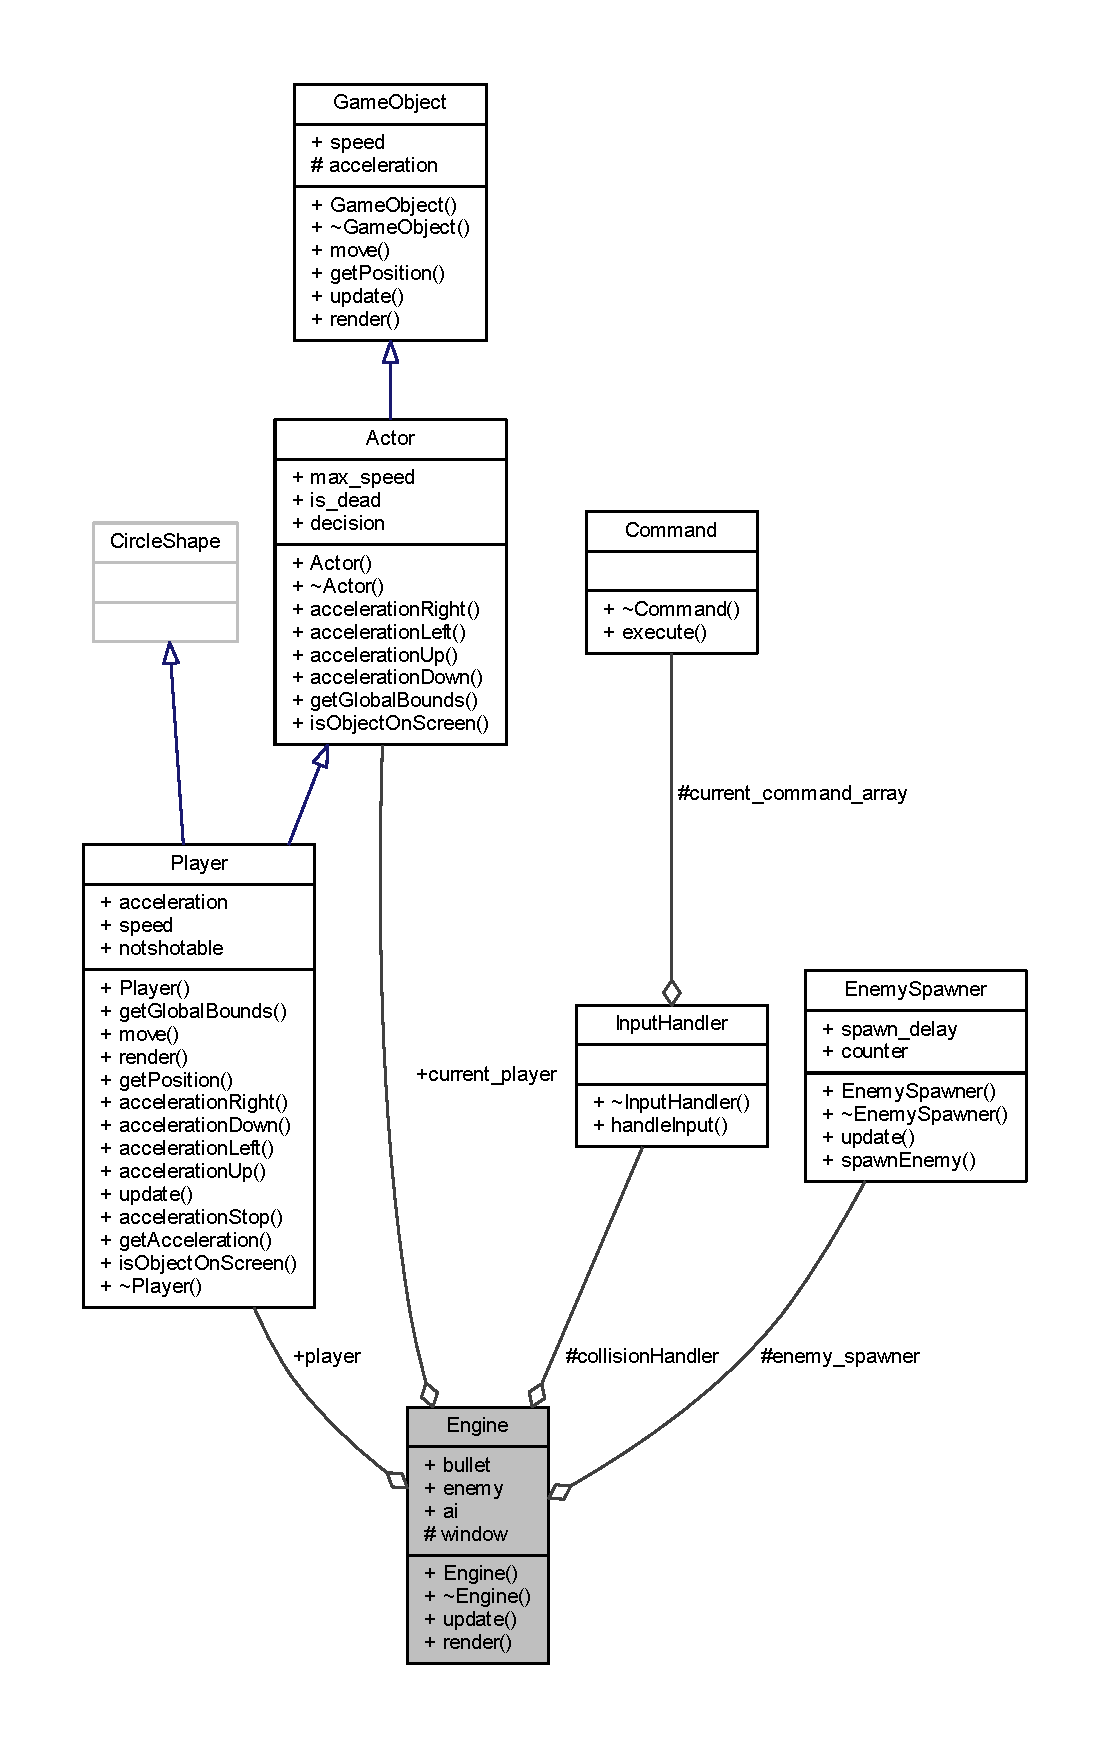
\includegraphics[height=550pt]{class_engine__coll__graph}
\end{center}
\end{figure}
\subsection*{Public Member Functions}
\begin{DoxyCompactItemize}
\item 
\hyperlink{class_engine_a74e8b812fd1bac60a35aaead9c3e81f8}{Engine} (sf\+::\+Render\+Window \&window\+\_\+in)
\item 
virtual \hyperlink{class_engine_a8ef7030a089ecb30bbfcb9e43094717a}{$\sim$\+Engine} ()
\item 
void \hyperlink{class_engine_ad2ff110d5a86c1cd60b541d65915ac48}{update} ()
\item 
void \hyperlink{class_engine_a7960743aefd62e846e7f3cd92c18bc73}{render} ()
\end{DoxyCompactItemize}
\subsection*{Public Attributes}
\begin{DoxyCompactItemize}
\item 
\hyperlink{class_player}{Player} \hyperlink{class_engine_abd0ff72a70b7643680cff6cd0513620f}{player}
\item 
\hyperlink{class_actor}{Actor} $\ast$ \hyperlink{class_engine_ab488c2946ac31376f272acc1eaf815b7}{current\+\_\+player}
\item 
std\+::vector$<$ \hyperlink{class_bullet}{Bullet} $\ast$ $>$ \hyperlink{class_engine_a267b13093cb4ea1de9c297a96b0314ea}{bullet}
\item 
std\+::vector$<$ \hyperlink{class_actor}{Actor} $\ast$ $>$ \hyperlink{class_engine_af5735da922e4f9fd64db49993dc8efe3}{enemy}
\item 
std\+::vector$<$ \hyperlink{class_ai_controler}{Ai\+Controler} $\ast$ $>$ \hyperlink{class_engine_a82c1ca4ee6f6dd4e9b79918aa12c156f}{ai}
\end{DoxyCompactItemize}
\subsection*{Protected Attributes}
\begin{DoxyCompactItemize}
\item 
sf\+::\+Render\+Window \& \hyperlink{class_engine_ae5fb055a0acce41034a9bff218dd87b1}{window}
\item 
\hyperlink{class_enemy_spawner}{Enemy\+Spawner} \hyperlink{class_engine_ac38501b7527b3c8ce22f8b31a13821ea}{enemy\+\_\+spawner}
\item 
std\+::unique\+\_\+ptr$<$ \hyperlink{class_input_handler}{Input\+Handler} $>$ \hyperlink{class_engine_a20fca6041ee94486e4ed1ec48d63dfef}{collision\+Handler}
\end{DoxyCompactItemize}


\subsection{Constructor \& Destructor Documentation}
\hypertarget{class_engine_a74e8b812fd1bac60a35aaead9c3e81f8}{}\index{Engine@{Engine}!Engine@{Engine}}
\index{Engine@{Engine}!Engine@{Engine}}
\subsubsection[{Engine}]{\setlength{\rightskip}{0pt plus 5cm}Engine\+::\+Engine (
\begin{DoxyParamCaption}
\item[{sf\+::\+Render\+Window \&}]{window\+\_\+in}
\end{DoxyParamCaption}
)}\label{class_engine_a74e8b812fd1bac60a35aaead9c3e81f8}
\hypertarget{class_engine_a8ef7030a089ecb30bbfcb9e43094717a}{}\index{Engine@{Engine}!````~Engine@{$\sim$\+Engine}}
\index{````~Engine@{$\sim$\+Engine}!Engine@{Engine}}
\subsubsection[{$\sim$\+Engine}]{\setlength{\rightskip}{0pt plus 5cm}Engine\+::$\sim$\+Engine (
\begin{DoxyParamCaption}
{}
\end{DoxyParamCaption}
)\hspace{0.3cm}{\ttfamily [virtual]}}\label{class_engine_a8ef7030a089ecb30bbfcb9e43094717a}


\subsection{Member Function Documentation}
\hypertarget{class_engine_a7960743aefd62e846e7f3cd92c18bc73}{}\index{Engine@{Engine}!render@{render}}
\index{render@{render}!Engine@{Engine}}
\subsubsection[{render}]{\setlength{\rightskip}{0pt plus 5cm}void Engine\+::render (
\begin{DoxyParamCaption}
{}
\end{DoxyParamCaption}
)}\label{class_engine_a7960743aefd62e846e7f3cd92c18bc73}
\hypertarget{class_engine_ad2ff110d5a86c1cd60b541d65915ac48}{}\index{Engine@{Engine}!update@{update}}
\index{update@{update}!Engine@{Engine}}
\subsubsection[{update}]{\setlength{\rightskip}{0pt plus 5cm}void Engine\+::update (
\begin{DoxyParamCaption}
{}
\end{DoxyParamCaption}
)}\label{class_engine_ad2ff110d5a86c1cd60b541d65915ac48}


Here is the call graph for this function\+:\nopagebreak
\begin{figure}[H]
\begin{center}
\leavevmode
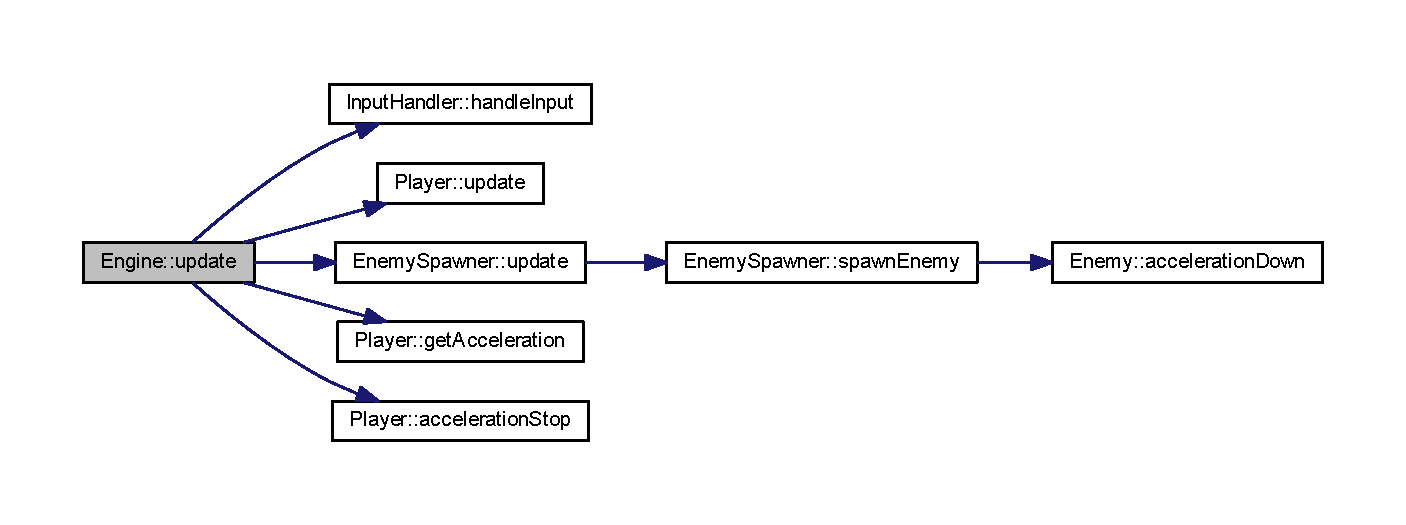
\includegraphics[width=350pt]{class_engine_ad2ff110d5a86c1cd60b541d65915ac48_cgraph}
\end{center}
\end{figure}




\subsection{Member Data Documentation}
\hypertarget{class_engine_a82c1ca4ee6f6dd4e9b79918aa12c156f}{}\index{Engine@{Engine}!ai@{ai}}
\index{ai@{ai}!Engine@{Engine}}
\subsubsection[{ai}]{\setlength{\rightskip}{0pt plus 5cm}std\+::vector$<${\bf Ai\+Controler}$\ast$$>$ Engine\+::ai}\label{class_engine_a82c1ca4ee6f6dd4e9b79918aa12c156f}
\hypertarget{class_engine_a267b13093cb4ea1de9c297a96b0314ea}{}\index{Engine@{Engine}!bullet@{bullet}}
\index{bullet@{bullet}!Engine@{Engine}}
\subsubsection[{bullet}]{\setlength{\rightskip}{0pt plus 5cm}std\+::vector$<${\bf Bullet}$\ast$$>$ Engine\+::bullet}\label{class_engine_a267b13093cb4ea1de9c297a96b0314ea}
\hypertarget{class_engine_a20fca6041ee94486e4ed1ec48d63dfef}{}\index{Engine@{Engine}!collision\+Handler@{collision\+Handler}}
\index{collision\+Handler@{collision\+Handler}!Engine@{Engine}}
\subsubsection[{collision\+Handler}]{\setlength{\rightskip}{0pt plus 5cm}std\+::unique\+\_\+ptr$<${\bf Input\+Handler}$>$ Engine\+::collision\+Handler\hspace{0.3cm}{\ttfamily [protected]}}\label{class_engine_a20fca6041ee94486e4ed1ec48d63dfef}
\hypertarget{class_engine_ab488c2946ac31376f272acc1eaf815b7}{}\index{Engine@{Engine}!current\+\_\+player@{current\+\_\+player}}
\index{current\+\_\+player@{current\+\_\+player}!Engine@{Engine}}
\subsubsection[{current\+\_\+player}]{\setlength{\rightskip}{0pt plus 5cm}{\bf Actor}$\ast$ Engine\+::current\+\_\+player}\label{class_engine_ab488c2946ac31376f272acc1eaf815b7}
\hypertarget{class_engine_af5735da922e4f9fd64db49993dc8efe3}{}\index{Engine@{Engine}!enemy@{enemy}}
\index{enemy@{enemy}!Engine@{Engine}}
\subsubsection[{enemy}]{\setlength{\rightskip}{0pt plus 5cm}std\+::vector$<${\bf Actor}$\ast$$>$ Engine\+::enemy}\label{class_engine_af5735da922e4f9fd64db49993dc8efe3}
\hypertarget{class_engine_ac38501b7527b3c8ce22f8b31a13821ea}{}\index{Engine@{Engine}!enemy\+\_\+spawner@{enemy\+\_\+spawner}}
\index{enemy\+\_\+spawner@{enemy\+\_\+spawner}!Engine@{Engine}}
\subsubsection[{enemy\+\_\+spawner}]{\setlength{\rightskip}{0pt plus 5cm}{\bf Enemy\+Spawner} Engine\+::enemy\+\_\+spawner\hspace{0.3cm}{\ttfamily [protected]}}\label{class_engine_ac38501b7527b3c8ce22f8b31a13821ea}
\hypertarget{class_engine_abd0ff72a70b7643680cff6cd0513620f}{}\index{Engine@{Engine}!player@{player}}
\index{player@{player}!Engine@{Engine}}
\subsubsection[{player}]{\setlength{\rightskip}{0pt plus 5cm}{\bf Player} Engine\+::player}\label{class_engine_abd0ff72a70b7643680cff6cd0513620f}
\hypertarget{class_engine_ae5fb055a0acce41034a9bff218dd87b1}{}\index{Engine@{Engine}!window@{window}}
\index{window@{window}!Engine@{Engine}}
\subsubsection[{window}]{\setlength{\rightskip}{0pt plus 5cm}sf\+::\+Render\+Window\& Engine\+::window\hspace{0.3cm}{\ttfamily [protected]}}\label{class_engine_ae5fb055a0acce41034a9bff218dd87b1}


The documentation for this class was generated from the following files\+:\begin{DoxyCompactItemize}
\item 
\hyperlink{_engine_8h}{Engine.\+h}\item 
\hyperlink{_engine_8cpp}{Engine.\+cpp}\end{DoxyCompactItemize}

\hypertarget{class_engine_input_handler}{}\section{Engine\+Input\+Handler Class Reference}
\label{class_engine_input_handler}\index{Engine\+Input\+Handler@{Engine\+Input\+Handler}}


{\ttfamily \#include $<$Engine\+Input\+Handler.\+h$>$}



Inheritance diagram for Engine\+Input\+Handler\+:
\nopagebreak
\begin{figure}[H]
\begin{center}
\leavevmode
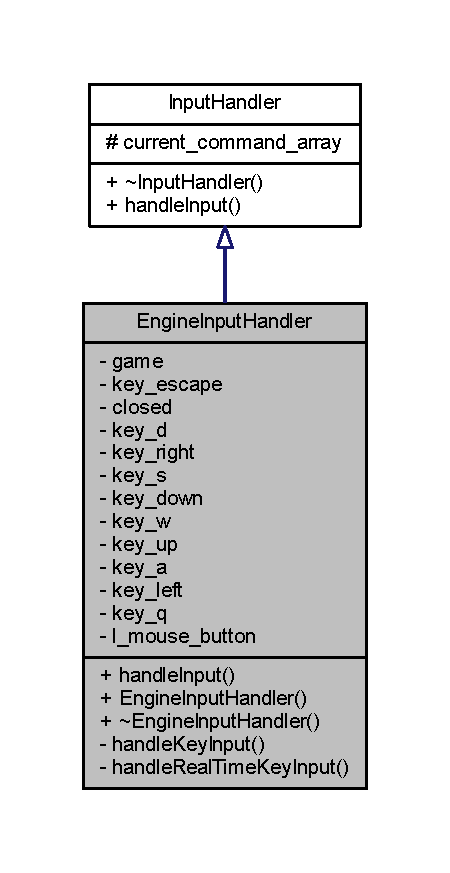
\includegraphics[width=216pt]{class_engine_input_handler__inherit__graph}
\end{center}
\end{figure}


Collaboration diagram for Engine\+Input\+Handler\+:
\nopagebreak
\begin{figure}[H]
\begin{center}
\leavevmode
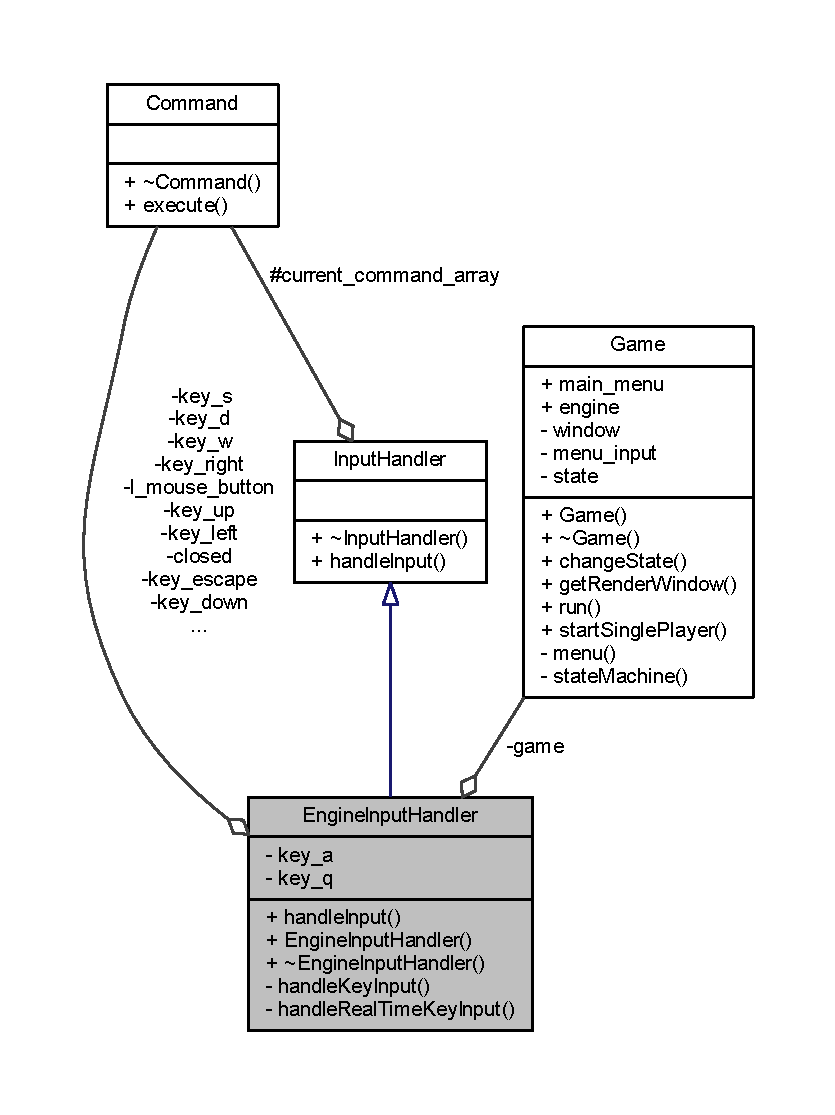
\includegraphics[width=350pt]{class_engine_input_handler__coll__graph}
\end{center}
\end{figure}
\subsection*{Public Member Functions}
\begin{DoxyCompactItemize}
\item 
\hyperlink{class_command}{Command} $\ast$$\ast$ \hyperlink{class_engine_input_handler_ade92afaf7657007c2be3b5bd745c96e3}{handle\+Input} () override
\item 
\hyperlink{class_engine_input_handler_ac33be38a17d38deb390b879ceb2e1e2f}{Engine\+Input\+Handler} (\hyperlink{class_game}{Game} \&game\+\_\+in)
\item 
virtual \hyperlink{class_engine_input_handler_a92a875197705110bd6b2debfe7dbee6a}{$\sim$\+Engine\+Input\+Handler} ()
\end{DoxyCompactItemize}
\subsection*{Private Member Functions}
\begin{DoxyCompactItemize}
\item 
\hyperlink{class_command}{Command} $\ast$ \hyperlink{class_engine_input_handler_a6b350fc8a379b04d36b2a60d4d673dcd}{handle\+Key\+Input} (sf\+::\+Event \&event, int \&i)
\item 
\hyperlink{class_command}{Command} $\ast$$\ast$ \hyperlink{class_engine_input_handler_a7e4a2c1a4cacf7ba3129c1e3a998de53}{handle\+Real\+Time\+Key\+Input} (sf\+::\+Event \&event, int \&i)
\end{DoxyCompactItemize}
\subsection*{Private Attributes}
\begin{DoxyCompactItemize}
\item 
\hyperlink{class_game}{Game} \& \hyperlink{class_engine_input_handler_a449d615b9968227381db153f57b7299d}{game}
\item 
\hyperlink{class_command}{Command} $\ast$ \hyperlink{class_engine_input_handler_ab64489773b1416e375218c236a22189a}{key\+\_\+escape}
\item 
\hyperlink{class_command}{Command} $\ast$ \hyperlink{class_engine_input_handler_ae7a6851ee3c22f14b78adc75de5cee56}{closed}
\item 
\hyperlink{class_command}{Command} $\ast$ \hyperlink{class_engine_input_handler_a0a8c3435c45eaa96f64c90476fe7f245}{key\+\_\+d}
\item 
\hyperlink{class_command}{Command} $\ast$ \hyperlink{class_engine_input_handler_a14eaaf6e8b2bcfe25cf1341e583bd830}{key\+\_\+right}
\item 
\hyperlink{class_command}{Command} $\ast$ \hyperlink{class_engine_input_handler_a59ae4ad6379aa180dcd7d858049dac62}{key\+\_\+s}
\item 
\hyperlink{class_command}{Command} $\ast$ \hyperlink{class_engine_input_handler_a863861091ad125fc57b72e319bd9b1e1}{key\+\_\+down}
\item 
\hyperlink{class_command}{Command} $\ast$ \hyperlink{class_engine_input_handler_a8be64818183cb4f9b906ff8694450d3e}{key\+\_\+w}
\item 
\hyperlink{class_command}{Command} $\ast$ \hyperlink{class_engine_input_handler_a46e2d81b780fe8bb344bb176ff2ee3a9}{key\+\_\+up}
\item 
\hyperlink{class_command}{Command} $\ast$ \hyperlink{class_engine_input_handler_a94fabe03a12102cec196570f7fb99dd0}{key\+\_\+a}
\item 
\hyperlink{class_command}{Command} $\ast$ \hyperlink{class_engine_input_handler_af778d434ad01423978eaecc5d392ba3b}{key\+\_\+left}
\item 
\hyperlink{class_command}{Command} $\ast$ \hyperlink{class_engine_input_handler_a0229e1c2b48f4049c77124aef8340909}{key\+\_\+q}
\item 
\hyperlink{class_command}{Command} $\ast$ \hyperlink{class_engine_input_handler_adf6145027b272f46e7c1381d4c905892}{l\+\_\+mouse\+\_\+button}
\end{DoxyCompactItemize}
\subsection*{Additional Inherited Members}


\subsection{Constructor \& Destructor Documentation}
\hypertarget{class_engine_input_handler_ac33be38a17d38deb390b879ceb2e1e2f}{}\index{Engine\+Input\+Handler@{Engine\+Input\+Handler}!Engine\+Input\+Handler@{Engine\+Input\+Handler}}
\index{Engine\+Input\+Handler@{Engine\+Input\+Handler}!Engine\+Input\+Handler@{Engine\+Input\+Handler}}
\subsubsection[{Engine\+Input\+Handler}]{\setlength{\rightskip}{0pt plus 5cm}Engine\+Input\+Handler\+::\+Engine\+Input\+Handler (
\begin{DoxyParamCaption}
\item[{{\bf Game} \&}]{game\+\_\+in}
\end{DoxyParamCaption}
)}\label{class_engine_input_handler_ac33be38a17d38deb390b879ceb2e1e2f}
\hypertarget{class_engine_input_handler_a92a875197705110bd6b2debfe7dbee6a}{}\index{Engine\+Input\+Handler@{Engine\+Input\+Handler}!````~Engine\+Input\+Handler@{$\sim$\+Engine\+Input\+Handler}}
\index{````~Engine\+Input\+Handler@{$\sim$\+Engine\+Input\+Handler}!Engine\+Input\+Handler@{Engine\+Input\+Handler}}
\subsubsection[{$\sim$\+Engine\+Input\+Handler}]{\setlength{\rightskip}{0pt plus 5cm}Engine\+Input\+Handler\+::$\sim$\+Engine\+Input\+Handler (
\begin{DoxyParamCaption}
{}
\end{DoxyParamCaption}
)\hspace{0.3cm}{\ttfamily [virtual]}}\label{class_engine_input_handler_a92a875197705110bd6b2debfe7dbee6a}


\subsection{Member Function Documentation}
\hypertarget{class_engine_input_handler_ade92afaf7657007c2be3b5bd745c96e3}{}\index{Engine\+Input\+Handler@{Engine\+Input\+Handler}!handle\+Input@{handle\+Input}}
\index{handle\+Input@{handle\+Input}!Engine\+Input\+Handler@{Engine\+Input\+Handler}}
\subsubsection[{handle\+Input}]{\setlength{\rightskip}{0pt plus 5cm}{\bf Command} $\ast$$\ast$ Engine\+Input\+Handler\+::handle\+Input (
\begin{DoxyParamCaption}
{}
\end{DoxyParamCaption}
)\hspace{0.3cm}{\ttfamily [override]}, {\ttfamily [virtual]}}\label{class_engine_input_handler_ade92afaf7657007c2be3b5bd745c96e3}


Implements \hyperlink{class_input_handler_a69b726d4a409a6f4ae443689cb69b404}{Input\+Handler}.



Here is the call graph for this function\+:
\nopagebreak
\begin{figure}[H]
\begin{center}
\leavevmode
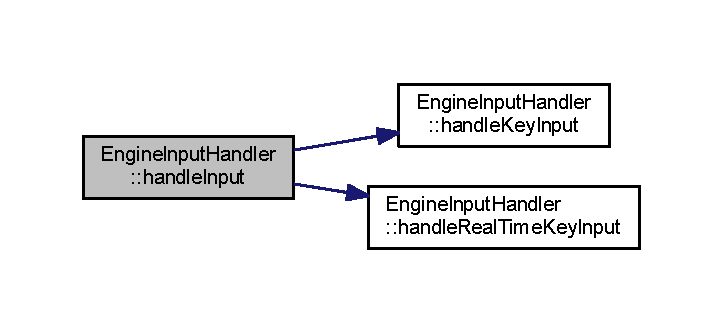
\includegraphics[width=347pt]{class_engine_input_handler_ade92afaf7657007c2be3b5bd745c96e3_cgraph}
\end{center}
\end{figure}


\hypertarget{class_engine_input_handler_a6b350fc8a379b04d36b2a60d4d673dcd}{}\index{Engine\+Input\+Handler@{Engine\+Input\+Handler}!handle\+Key\+Input@{handle\+Key\+Input}}
\index{handle\+Key\+Input@{handle\+Key\+Input}!Engine\+Input\+Handler@{Engine\+Input\+Handler}}
\subsubsection[{handle\+Key\+Input}]{\setlength{\rightskip}{0pt plus 5cm}{\bf Command} $\ast$ Engine\+Input\+Handler\+::handle\+Key\+Input (
\begin{DoxyParamCaption}
\item[{sf\+::\+Event \&}]{event, }
\item[{int \&}]{i}
\end{DoxyParamCaption}
)\hspace{0.3cm}{\ttfamily [private]}}\label{class_engine_input_handler_a6b350fc8a379b04d36b2a60d4d673dcd}


Here is the caller graph for this function\+:
\nopagebreak
\begin{figure}[H]
\begin{center}
\leavevmode
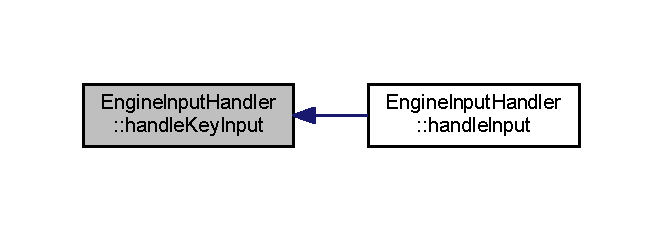
\includegraphics[width=318pt]{class_engine_input_handler_a6b350fc8a379b04d36b2a60d4d673dcd_icgraph}
\end{center}
\end{figure}


\hypertarget{class_engine_input_handler_a7e4a2c1a4cacf7ba3129c1e3a998de53}{}\index{Engine\+Input\+Handler@{Engine\+Input\+Handler}!handle\+Real\+Time\+Key\+Input@{handle\+Real\+Time\+Key\+Input}}
\index{handle\+Real\+Time\+Key\+Input@{handle\+Real\+Time\+Key\+Input}!Engine\+Input\+Handler@{Engine\+Input\+Handler}}
\subsubsection[{handle\+Real\+Time\+Key\+Input}]{\setlength{\rightskip}{0pt plus 5cm}{\bf Command} $\ast$$\ast$ Engine\+Input\+Handler\+::handle\+Real\+Time\+Key\+Input (
\begin{DoxyParamCaption}
\item[{sf\+::\+Event \&}]{event, }
\item[{int \&}]{i}
\end{DoxyParamCaption}
)\hspace{0.3cm}{\ttfamily [private]}}\label{class_engine_input_handler_a7e4a2c1a4cacf7ba3129c1e3a998de53}


Here is the caller graph for this function\+:
\nopagebreak
\begin{figure}[H]
\begin{center}
\leavevmode
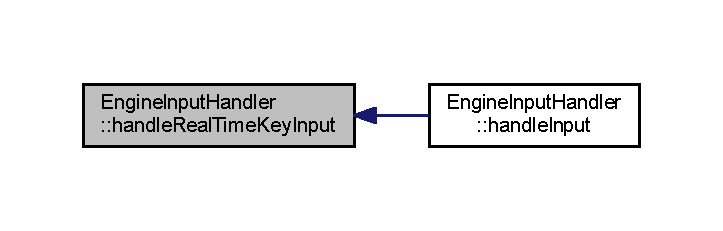
\includegraphics[width=347pt]{class_engine_input_handler_a7e4a2c1a4cacf7ba3129c1e3a998de53_icgraph}
\end{center}
\end{figure}




\subsection{Member Data Documentation}
\hypertarget{class_engine_input_handler_ae7a6851ee3c22f14b78adc75de5cee56}{}\index{Engine\+Input\+Handler@{Engine\+Input\+Handler}!closed@{closed}}
\index{closed@{closed}!Engine\+Input\+Handler@{Engine\+Input\+Handler}}
\subsubsection[{closed}]{\setlength{\rightskip}{0pt plus 5cm}{\bf Command}$\ast$ Engine\+Input\+Handler\+::closed\hspace{0.3cm}{\ttfamily [private]}}\label{class_engine_input_handler_ae7a6851ee3c22f14b78adc75de5cee56}
\hypertarget{class_engine_input_handler_a449d615b9968227381db153f57b7299d}{}\index{Engine\+Input\+Handler@{Engine\+Input\+Handler}!game@{game}}
\index{game@{game}!Engine\+Input\+Handler@{Engine\+Input\+Handler}}
\subsubsection[{game}]{\setlength{\rightskip}{0pt plus 5cm}{\bf Game}\& Engine\+Input\+Handler\+::game\hspace{0.3cm}{\ttfamily [private]}}\label{class_engine_input_handler_a449d615b9968227381db153f57b7299d}
\hypertarget{class_engine_input_handler_a94fabe03a12102cec196570f7fb99dd0}{}\index{Engine\+Input\+Handler@{Engine\+Input\+Handler}!key\+\_\+a@{key\+\_\+a}}
\index{key\+\_\+a@{key\+\_\+a}!Engine\+Input\+Handler@{Engine\+Input\+Handler}}
\subsubsection[{key\+\_\+a}]{\setlength{\rightskip}{0pt plus 5cm}{\bf Command}$\ast$ Engine\+Input\+Handler\+::key\+\_\+a\hspace{0.3cm}{\ttfamily [private]}}\label{class_engine_input_handler_a94fabe03a12102cec196570f7fb99dd0}
\hypertarget{class_engine_input_handler_a0a8c3435c45eaa96f64c90476fe7f245}{}\index{Engine\+Input\+Handler@{Engine\+Input\+Handler}!key\+\_\+d@{key\+\_\+d}}
\index{key\+\_\+d@{key\+\_\+d}!Engine\+Input\+Handler@{Engine\+Input\+Handler}}
\subsubsection[{key\+\_\+d}]{\setlength{\rightskip}{0pt plus 5cm}{\bf Command}$\ast$ Engine\+Input\+Handler\+::key\+\_\+d\hspace{0.3cm}{\ttfamily [private]}}\label{class_engine_input_handler_a0a8c3435c45eaa96f64c90476fe7f245}
\hypertarget{class_engine_input_handler_a863861091ad125fc57b72e319bd9b1e1}{}\index{Engine\+Input\+Handler@{Engine\+Input\+Handler}!key\+\_\+down@{key\+\_\+down}}
\index{key\+\_\+down@{key\+\_\+down}!Engine\+Input\+Handler@{Engine\+Input\+Handler}}
\subsubsection[{key\+\_\+down}]{\setlength{\rightskip}{0pt plus 5cm}{\bf Command}$\ast$ Engine\+Input\+Handler\+::key\+\_\+down\hspace{0.3cm}{\ttfamily [private]}}\label{class_engine_input_handler_a863861091ad125fc57b72e319bd9b1e1}
\hypertarget{class_engine_input_handler_ab64489773b1416e375218c236a22189a}{}\index{Engine\+Input\+Handler@{Engine\+Input\+Handler}!key\+\_\+escape@{key\+\_\+escape}}
\index{key\+\_\+escape@{key\+\_\+escape}!Engine\+Input\+Handler@{Engine\+Input\+Handler}}
\subsubsection[{key\+\_\+escape}]{\setlength{\rightskip}{0pt plus 5cm}{\bf Command}$\ast$ Engine\+Input\+Handler\+::key\+\_\+escape\hspace{0.3cm}{\ttfamily [private]}}\label{class_engine_input_handler_ab64489773b1416e375218c236a22189a}
\hypertarget{class_engine_input_handler_af778d434ad01423978eaecc5d392ba3b}{}\index{Engine\+Input\+Handler@{Engine\+Input\+Handler}!key\+\_\+left@{key\+\_\+left}}
\index{key\+\_\+left@{key\+\_\+left}!Engine\+Input\+Handler@{Engine\+Input\+Handler}}
\subsubsection[{key\+\_\+left}]{\setlength{\rightskip}{0pt plus 5cm}{\bf Command}$\ast$ Engine\+Input\+Handler\+::key\+\_\+left\hspace{0.3cm}{\ttfamily [private]}}\label{class_engine_input_handler_af778d434ad01423978eaecc5d392ba3b}
\hypertarget{class_engine_input_handler_a0229e1c2b48f4049c77124aef8340909}{}\index{Engine\+Input\+Handler@{Engine\+Input\+Handler}!key\+\_\+q@{key\+\_\+q}}
\index{key\+\_\+q@{key\+\_\+q}!Engine\+Input\+Handler@{Engine\+Input\+Handler}}
\subsubsection[{key\+\_\+q}]{\setlength{\rightskip}{0pt plus 5cm}{\bf Command}$\ast$ Engine\+Input\+Handler\+::key\+\_\+q\hspace{0.3cm}{\ttfamily [private]}}\label{class_engine_input_handler_a0229e1c2b48f4049c77124aef8340909}
\hypertarget{class_engine_input_handler_a14eaaf6e8b2bcfe25cf1341e583bd830}{}\index{Engine\+Input\+Handler@{Engine\+Input\+Handler}!key\+\_\+right@{key\+\_\+right}}
\index{key\+\_\+right@{key\+\_\+right}!Engine\+Input\+Handler@{Engine\+Input\+Handler}}
\subsubsection[{key\+\_\+right}]{\setlength{\rightskip}{0pt plus 5cm}{\bf Command}$\ast$ Engine\+Input\+Handler\+::key\+\_\+right\hspace{0.3cm}{\ttfamily [private]}}\label{class_engine_input_handler_a14eaaf6e8b2bcfe25cf1341e583bd830}
\hypertarget{class_engine_input_handler_a59ae4ad6379aa180dcd7d858049dac62}{}\index{Engine\+Input\+Handler@{Engine\+Input\+Handler}!key\+\_\+s@{key\+\_\+s}}
\index{key\+\_\+s@{key\+\_\+s}!Engine\+Input\+Handler@{Engine\+Input\+Handler}}
\subsubsection[{key\+\_\+s}]{\setlength{\rightskip}{0pt plus 5cm}{\bf Command}$\ast$ Engine\+Input\+Handler\+::key\+\_\+s\hspace{0.3cm}{\ttfamily [private]}}\label{class_engine_input_handler_a59ae4ad6379aa180dcd7d858049dac62}
\hypertarget{class_engine_input_handler_a46e2d81b780fe8bb344bb176ff2ee3a9}{}\index{Engine\+Input\+Handler@{Engine\+Input\+Handler}!key\+\_\+up@{key\+\_\+up}}
\index{key\+\_\+up@{key\+\_\+up}!Engine\+Input\+Handler@{Engine\+Input\+Handler}}
\subsubsection[{key\+\_\+up}]{\setlength{\rightskip}{0pt plus 5cm}{\bf Command}$\ast$ Engine\+Input\+Handler\+::key\+\_\+up\hspace{0.3cm}{\ttfamily [private]}}\label{class_engine_input_handler_a46e2d81b780fe8bb344bb176ff2ee3a9}
\hypertarget{class_engine_input_handler_a8be64818183cb4f9b906ff8694450d3e}{}\index{Engine\+Input\+Handler@{Engine\+Input\+Handler}!key\+\_\+w@{key\+\_\+w}}
\index{key\+\_\+w@{key\+\_\+w}!Engine\+Input\+Handler@{Engine\+Input\+Handler}}
\subsubsection[{key\+\_\+w}]{\setlength{\rightskip}{0pt plus 5cm}{\bf Command}$\ast$ Engine\+Input\+Handler\+::key\+\_\+w\hspace{0.3cm}{\ttfamily [private]}}\label{class_engine_input_handler_a8be64818183cb4f9b906ff8694450d3e}
\hypertarget{class_engine_input_handler_adf6145027b272f46e7c1381d4c905892}{}\index{Engine\+Input\+Handler@{Engine\+Input\+Handler}!l\+\_\+mouse\+\_\+button@{l\+\_\+mouse\+\_\+button}}
\index{l\+\_\+mouse\+\_\+button@{l\+\_\+mouse\+\_\+button}!Engine\+Input\+Handler@{Engine\+Input\+Handler}}
\subsubsection[{l\+\_\+mouse\+\_\+button}]{\setlength{\rightskip}{0pt plus 5cm}{\bf Command}$\ast$ Engine\+Input\+Handler\+::l\+\_\+mouse\+\_\+button\hspace{0.3cm}{\ttfamily [private]}}\label{class_engine_input_handler_adf6145027b272f46e7c1381d4c905892}


The documentation for this class was generated from the following files\+:\begin{DoxyCompactItemize}
\item 
\hyperlink{_engine_input_handler_8h}{Engine\+Input\+Handler.\+h}\item 
\hyperlink{_engine_input_handler_8cpp}{Engine\+Input\+Handler.\+cpp}\end{DoxyCompactItemize}

\hypertarget{class_enter_choice_command}{}\section{Enter\+Choice\+Command Class Reference}
\label{class_enter_choice_command}\index{Enter\+Choice\+Command@{Enter\+Choice\+Command}}


{\ttfamily \#include $<$Enter\+Choice\+Command.\+h$>$}



Inheritance diagram for Enter\+Choice\+Command\+:\nopagebreak
\begin{figure}[H]
\begin{center}
\leavevmode
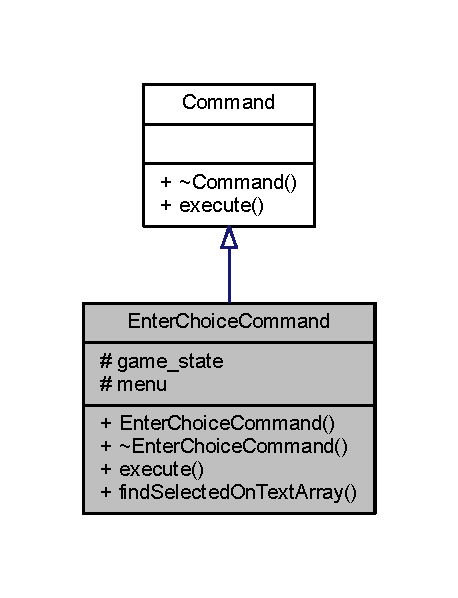
\includegraphics[width=220pt]{class_enter_choice_command__inherit__graph}
\end{center}
\end{figure}


Collaboration diagram for Enter\+Choice\+Command\+:\nopagebreak
\begin{figure}[H]
\begin{center}
\leavevmode
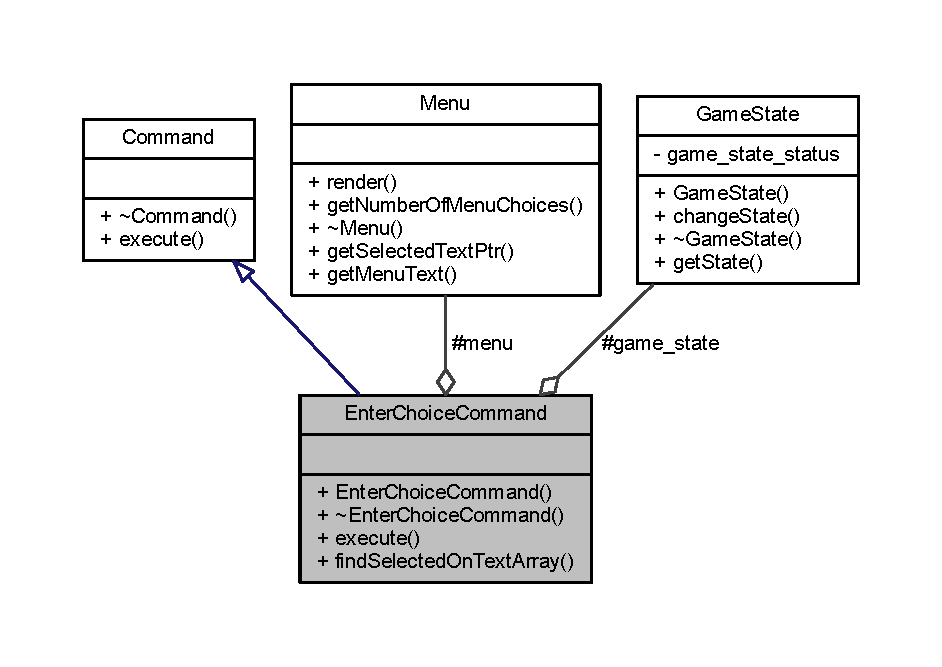
\includegraphics[width=290pt]{class_enter_choice_command__coll__graph}
\end{center}
\end{figure}
\subsection*{Public Member Functions}
\begin{DoxyCompactItemize}
\item 
\hyperlink{class_enter_choice_command_ab28cfc3f238985775ec33ebb33c355a6}{Enter\+Choice\+Command} (\hyperlink{class_game}{Game} \&game\+\_\+in)
\item 
virtual \hyperlink{class_enter_choice_command_aa7a330dcd6ffcf6f806c26b577bba21c}{$\sim$\+Enter\+Choice\+Command} ()
\item 
void \hyperlink{class_enter_choice_command_a684f65bfc296353ecefc6edc1c678c70}{execute} () override
\item 
int \hyperlink{class_enter_choice_command_a09b35eafcb1ba6d9e6fb93425702e6c4}{find\+Selected\+On\+Text\+Array} ()
\end{DoxyCompactItemize}
\subsection*{Protected Attributes}
\begin{DoxyCompactItemize}
\item 
\hyperlink{class_game}{Game} \& \hyperlink{class_enter_choice_command_a53c2b9d8c1ee8b9bdbed6ad4889f10b0}{game}
\end{DoxyCompactItemize}


\subsection{Constructor \& Destructor Documentation}
\hypertarget{class_enter_choice_command_ab28cfc3f238985775ec33ebb33c355a6}{}\index{Enter\+Choice\+Command@{Enter\+Choice\+Command}!Enter\+Choice\+Command@{Enter\+Choice\+Command}}
\index{Enter\+Choice\+Command@{Enter\+Choice\+Command}!Enter\+Choice\+Command@{Enter\+Choice\+Command}}
\subsubsection[{Enter\+Choice\+Command}]{\setlength{\rightskip}{0pt plus 5cm}Enter\+Choice\+Command\+::\+Enter\+Choice\+Command (
\begin{DoxyParamCaption}
\item[{{\bf Game} \&}]{game\+\_\+in}
\end{DoxyParamCaption}
)}\label{class_enter_choice_command_ab28cfc3f238985775ec33ebb33c355a6}
\hypertarget{class_enter_choice_command_aa7a330dcd6ffcf6f806c26b577bba21c}{}\index{Enter\+Choice\+Command@{Enter\+Choice\+Command}!````~Enter\+Choice\+Command@{$\sim$\+Enter\+Choice\+Command}}
\index{````~Enter\+Choice\+Command@{$\sim$\+Enter\+Choice\+Command}!Enter\+Choice\+Command@{Enter\+Choice\+Command}}
\subsubsection[{$\sim$\+Enter\+Choice\+Command}]{\setlength{\rightskip}{0pt plus 5cm}Enter\+Choice\+Command\+::$\sim$\+Enter\+Choice\+Command (
\begin{DoxyParamCaption}
{}
\end{DoxyParamCaption}
)\hspace{0.3cm}{\ttfamily [virtual]}}\label{class_enter_choice_command_aa7a330dcd6ffcf6f806c26b577bba21c}


\subsection{Member Function Documentation}
\hypertarget{class_enter_choice_command_a684f65bfc296353ecefc6edc1c678c70}{}\index{Enter\+Choice\+Command@{Enter\+Choice\+Command}!execute@{execute}}
\index{execute@{execute}!Enter\+Choice\+Command@{Enter\+Choice\+Command}}
\subsubsection[{execute}]{\setlength{\rightskip}{0pt plus 5cm}void Enter\+Choice\+Command\+::execute (
\begin{DoxyParamCaption}
{}
\end{DoxyParamCaption}
)\hspace{0.3cm}{\ttfamily [override]}, {\ttfamily [virtual]}}\label{class_enter_choice_command_a684f65bfc296353ecefc6edc1c678c70}


Implements \hyperlink{class_command_a6fd7d9bd8df8bfc881e4d6c7cd1878b7}{Command}.



Here is the call graph for this function\+:\nopagebreak
\begin{figure}[H]
\begin{center}
\leavevmode
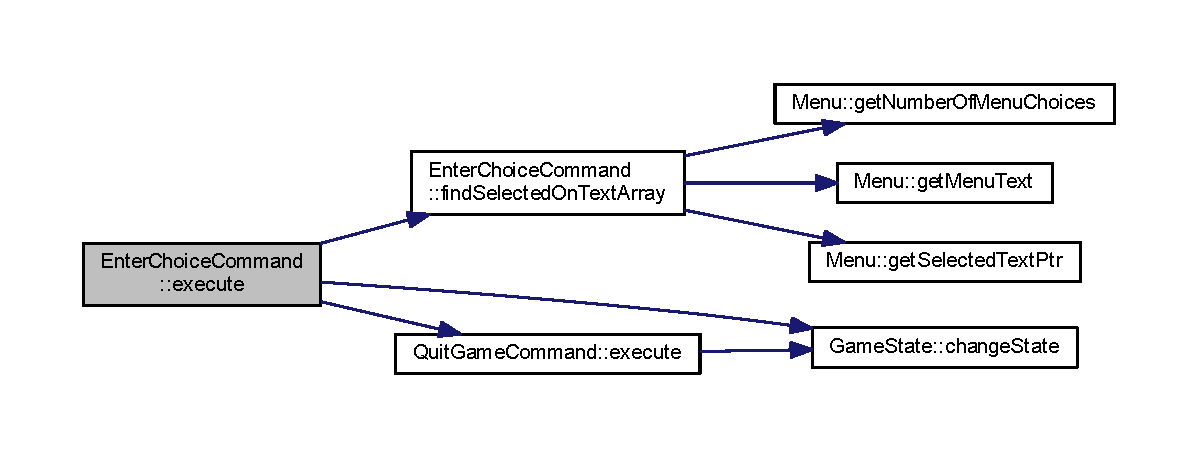
\includegraphics[width=350pt]{class_enter_choice_command_a684f65bfc296353ecefc6edc1c678c70_cgraph}
\end{center}
\end{figure}


\hypertarget{class_enter_choice_command_a09b35eafcb1ba6d9e6fb93425702e6c4}{}\index{Enter\+Choice\+Command@{Enter\+Choice\+Command}!find\+Selected\+On\+Text\+Array@{find\+Selected\+On\+Text\+Array}}
\index{find\+Selected\+On\+Text\+Array@{find\+Selected\+On\+Text\+Array}!Enter\+Choice\+Command@{Enter\+Choice\+Command}}
\subsubsection[{find\+Selected\+On\+Text\+Array}]{\setlength{\rightskip}{0pt plus 5cm}int Enter\+Choice\+Command\+::find\+Selected\+On\+Text\+Array (
\begin{DoxyParamCaption}
{}
\end{DoxyParamCaption}
)}\label{class_enter_choice_command_a09b35eafcb1ba6d9e6fb93425702e6c4}


Here is the caller graph for this function\+:\nopagebreak
\begin{figure}[H]
\begin{center}
\leavevmode
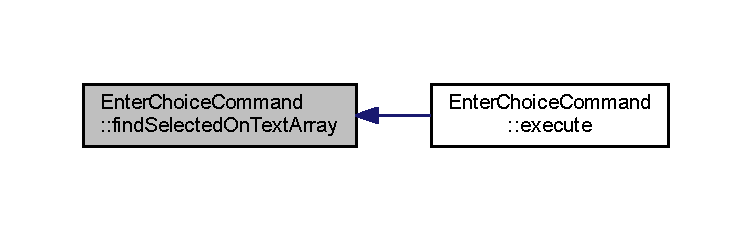
\includegraphics[width=350pt]{class_enter_choice_command_a09b35eafcb1ba6d9e6fb93425702e6c4_icgraph}
\end{center}
\end{figure}




\subsection{Member Data Documentation}
\hypertarget{class_enter_choice_command_a53c2b9d8c1ee8b9bdbed6ad4889f10b0}{}\index{Enter\+Choice\+Command@{Enter\+Choice\+Command}!game@{game}}
\index{game@{game}!Enter\+Choice\+Command@{Enter\+Choice\+Command}}
\subsubsection[{game}]{\setlength{\rightskip}{0pt plus 5cm}{\bf Game}\& Enter\+Choice\+Command\+::game\hspace{0.3cm}{\ttfamily [protected]}}\label{class_enter_choice_command_a53c2b9d8c1ee8b9bdbed6ad4889f10b0}


The documentation for this class was generated from the following files\+:\begin{DoxyCompactItemize}
\item 
\hyperlink{_enter_choice_command_8h}{Enter\+Choice\+Command.\+h}\item 
\hyperlink{_enter_choice_command_8cpp}{Enter\+Choice\+Command.\+cpp}\end{DoxyCompactItemize}

\hypertarget{class_game}{}\section{Game Class Reference}
\label{class_game}\index{Game@{Game}}


\hyperlink{class_game}{Game} main class. Class which is used run engine. This class will menage menu and settings.  




{\ttfamily \#include $<$Game.\+h$>$}



Collaboration diagram for Game\+:\nopagebreak
\begin{figure}[H]
\begin{center}
\leavevmode
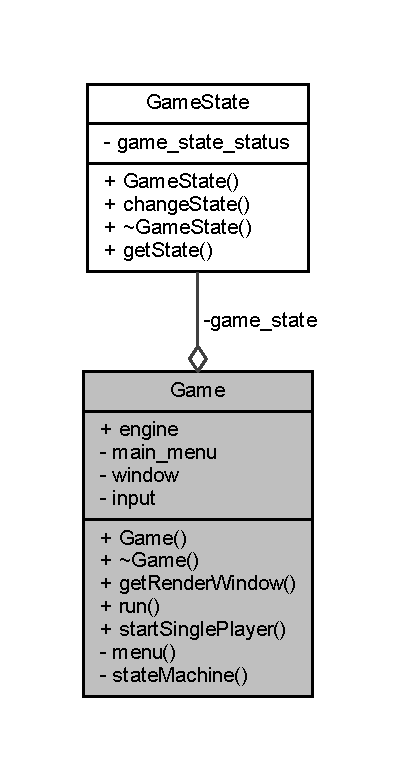
\includegraphics[width=190pt]{class_game__coll__graph}
\end{center}
\end{figure}
\subsection*{Public Types}
\begin{DoxyCompactItemize}
\item 
enum \hyperlink{class_game_a7f57a7a8408e554d0a72882c287e1d04}{Game\+State} \{ \hyperlink{class_game_a7f57a7a8408e554d0a72882c287e1d04a7a51f25e2194782f14973800a89e58fd}{Menu\+State}, 
\hyperlink{class_game_a7f57a7a8408e554d0a72882c287e1d04a08c295bf12e492bf9d64b14d8d83b736}{Play\+Single\+State}, 
\hyperlink{class_game_a7f57a7a8408e554d0a72882c287e1d04afc92d30e44f9ec0ff71b695a3ec6d5ca}{End\+State}
 \}
\end{DoxyCompactItemize}
\subsection*{Public Member Functions}
\begin{DoxyCompactItemize}
\item 
\hyperlink{class_game_a0010695fcd27f6fc91b37b5cf3ed0543}{Game} (sf\+::\+Render\+Window \&window\+\_\+in)
\begin{DoxyCompactList}\small\item\em Initialization of Render\+Window\& window -\/ main window of the game. \end{DoxyCompactList}\item 
virtual \hyperlink{class_game_ae3d112ca6e0e55150d2fdbc704474530}{$\sim$\+Game} ()
\begin{DoxyCompactList}\small\item\em Runs Start\+Game() function. \end{DoxyCompactList}\item 
void \hyperlink{class_game_a82e2140cdedd171aecaed897d3aea5a0}{change\+State} (\hyperlink{class_game_a7f57a7a8408e554d0a72882c287e1d04}{Game\+State} new\+\_\+state)
\item 
sf\+::\+Render\+Window \& \hyperlink{class_game_ada9faa2a1f4e1453420adead02fd9865}{get\+Render\+Window} ()
\item 
void \hyperlink{class_game_a1ab78f5ed0d5ea879157357cf2fb2afa}{run} ()
\item 
void \hyperlink{class_game_afbc524f7661c9ce1bea6ca45fd212093}{start\+Single\+Player} ()
\end{DoxyCompactItemize}
\subsection*{Public Attributes}
\begin{DoxyCompactItemize}
\item 
std\+::unique\+\_\+ptr$<$ \hyperlink{class_menu}{Menu} $>$ \hyperlink{class_game_ae08cf171b4f973d47def68d69f561e2c}{main\+\_\+menu}
\item 
std\+::unique\+\_\+ptr$<$ \hyperlink{class_engine}{Engine} $>$ \hyperlink{class_game_aee6b9ebe224001f736e1ed71a3b28223}{engine}
\end{DoxyCompactItemize}
\subsection*{Private Member Functions}
\begin{DoxyCompactItemize}
\item 
void \hyperlink{class_game_a463932fa7ca2f1ce243279bf2422fc48}{menu} ()
\item 
void \hyperlink{class_game_a8bc94200bfbf0421b83b7c2b2b45da72}{state\+Machine} ()
\end{DoxyCompactItemize}
\subsection*{Private Attributes}
\begin{DoxyCompactItemize}
\item 
sf\+::\+Render\+Window \& \hyperlink{class_game_ad0fb4d8653dcf289fd6573cf5ba0f3d1}{window}
\begin{DoxyCompactList}\small\item\em Main game window. \end{DoxyCompactList}\item 
std\+::unique\+\_\+ptr$<$ \hyperlink{class_input_handler}{Input\+Handler} $>$ \hyperlink{class_game_a82776f65732ac43cf35b8b7c7120c873}{menu\+\_\+input}
\item 
\hyperlink{class_game_a7f57a7a8408e554d0a72882c287e1d04}{Game\+State} \hyperlink{class_game_ad9fc2a8710ee56916f79314b91112ed0}{state}
\end{DoxyCompactItemize}


\subsection{Detailed Description}
\hyperlink{class_game}{Game} main class. Class which is used run engine. This class will menage menu and settings. 

\subsection{Member Enumeration Documentation}
\hypertarget{class_game_a7f57a7a8408e554d0a72882c287e1d04}{}\index{Game@{Game}!Game\+State@{Game\+State}}
\index{Game\+State@{Game\+State}!Game@{Game}}
\subsubsection[{Game\+State}]{\setlength{\rightskip}{0pt plus 5cm}enum {\bf Game\+::\+Game\+State}}\label{class_game_a7f57a7a8408e554d0a72882c287e1d04}
\begin{Desc}
\item[Enumerator]\par
\begin{description}
\index{Menu\+State@{Menu\+State}!Game@{Game}}\index{Game@{Game}!Menu\+State@{Menu\+State}}\item[{\em 
\hypertarget{class_game_a7f57a7a8408e554d0a72882c287e1d04a7a51f25e2194782f14973800a89e58fd}{}Menu\+State\label{class_game_a7f57a7a8408e554d0a72882c287e1d04a7a51f25e2194782f14973800a89e58fd}
}]\index{Play\+Single\+State@{Play\+Single\+State}!Game@{Game}}\index{Game@{Game}!Play\+Single\+State@{Play\+Single\+State}}\item[{\em 
\hypertarget{class_game_a7f57a7a8408e554d0a72882c287e1d04a08c295bf12e492bf9d64b14d8d83b736}{}Play\+Single\+State\label{class_game_a7f57a7a8408e554d0a72882c287e1d04a08c295bf12e492bf9d64b14d8d83b736}
}]\index{End\+State@{End\+State}!Game@{Game}}\index{Game@{Game}!End\+State@{End\+State}}\item[{\em 
\hypertarget{class_game_a7f57a7a8408e554d0a72882c287e1d04afc92d30e44f9ec0ff71b695a3ec6d5ca}{}End\+State\label{class_game_a7f57a7a8408e554d0a72882c287e1d04afc92d30e44f9ec0ff71b695a3ec6d5ca}
}]\end{description}
\end{Desc}


\subsection{Constructor \& Destructor Documentation}
\hypertarget{class_game_a0010695fcd27f6fc91b37b5cf3ed0543}{}\index{Game@{Game}!Game@{Game}}
\index{Game@{Game}!Game@{Game}}
\subsubsection[{Game}]{\setlength{\rightskip}{0pt plus 5cm}Game\+::\+Game (
\begin{DoxyParamCaption}
\item[{sf\+::\+Render\+Window \&}]{window\+\_\+in}
\end{DoxyParamCaption}
)}\label{class_game_a0010695fcd27f6fc91b37b5cf3ed0543}


Initialization of Render\+Window\& window -\/ main window of the game. 

\hypertarget{class_game_ae3d112ca6e0e55150d2fdbc704474530}{}\index{Game@{Game}!````~Game@{$\sim$\+Game}}
\index{````~Game@{$\sim$\+Game}!Game@{Game}}
\subsubsection[{$\sim$\+Game}]{\setlength{\rightskip}{0pt plus 5cm}Game\+::$\sim$\+Game (
\begin{DoxyParamCaption}
{}
\end{DoxyParamCaption}
)\hspace{0.3cm}{\ttfamily [virtual]}}\label{class_game_ae3d112ca6e0e55150d2fdbc704474530}


Runs Start\+Game() function. 



\subsection{Member Function Documentation}
\hypertarget{class_game_a82e2140cdedd171aecaed897d3aea5a0}{}\index{Game@{Game}!change\+State@{change\+State}}
\index{change\+State@{change\+State}!Game@{Game}}
\subsubsection[{change\+State}]{\setlength{\rightskip}{0pt plus 5cm}void Game\+::change\+State (
\begin{DoxyParamCaption}
\item[{{\bf Game\+State}}]{new\+\_\+state}
\end{DoxyParamCaption}
)}\label{class_game_a82e2140cdedd171aecaed897d3aea5a0}


Here is the caller graph for this function\+:\nopagebreak
\begin{figure}[H]
\begin{center}
\leavevmode
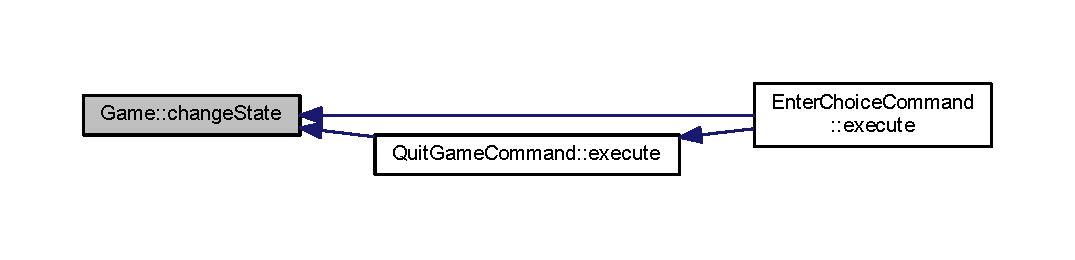
\includegraphics[width=350pt]{class_game_a82e2140cdedd171aecaed897d3aea5a0_icgraph}
\end{center}
\end{figure}


\hypertarget{class_game_ada9faa2a1f4e1453420adead02fd9865}{}\index{Game@{Game}!get\+Render\+Window@{get\+Render\+Window}}
\index{get\+Render\+Window@{get\+Render\+Window}!Game@{Game}}
\subsubsection[{get\+Render\+Window}]{\setlength{\rightskip}{0pt plus 5cm}sf\+::\+Render\+Window \& Game\+::get\+Render\+Window (
\begin{DoxyParamCaption}
{}
\end{DoxyParamCaption}
)}\label{class_game_ada9faa2a1f4e1453420adead02fd9865}


Here is the caller graph for this function\+:\nopagebreak
\begin{figure}[H]
\begin{center}
\leavevmode
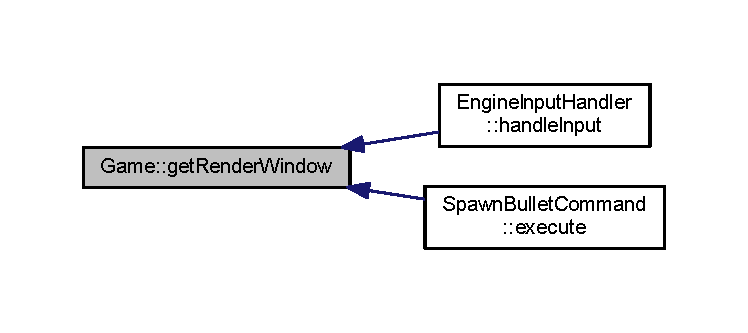
\includegraphics[width=350pt]{class_game_ada9faa2a1f4e1453420adead02fd9865_icgraph}
\end{center}
\end{figure}


\hypertarget{class_game_a463932fa7ca2f1ce243279bf2422fc48}{}\index{Game@{Game}!menu@{menu}}
\index{menu@{menu}!Game@{Game}}
\subsubsection[{menu}]{\setlength{\rightskip}{0pt plus 5cm}void Game\+::menu (
\begin{DoxyParamCaption}
{}
\end{DoxyParamCaption}
)\hspace{0.3cm}{\ttfamily [private]}}\label{class_game_a463932fa7ca2f1ce243279bf2422fc48}


Here is the caller graph for this function\+:\nopagebreak
\begin{figure}[H]
\begin{center}
\leavevmode
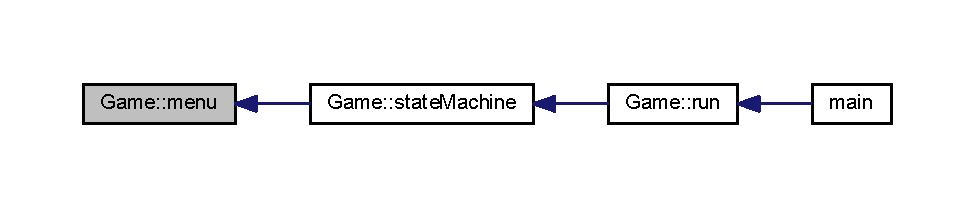
\includegraphics[width=350pt]{class_game_a463932fa7ca2f1ce243279bf2422fc48_icgraph}
\end{center}
\end{figure}


\hypertarget{class_game_a1ab78f5ed0d5ea879157357cf2fb2afa}{}\index{Game@{Game}!run@{run}}
\index{run@{run}!Game@{Game}}
\subsubsection[{run}]{\setlength{\rightskip}{0pt plus 5cm}void Game\+::run (
\begin{DoxyParamCaption}
{}
\end{DoxyParamCaption}
)}\label{class_game_a1ab78f5ed0d5ea879157357cf2fb2afa}


Here is the call graph for this function\+:\nopagebreak
\begin{figure}[H]
\begin{center}
\leavevmode
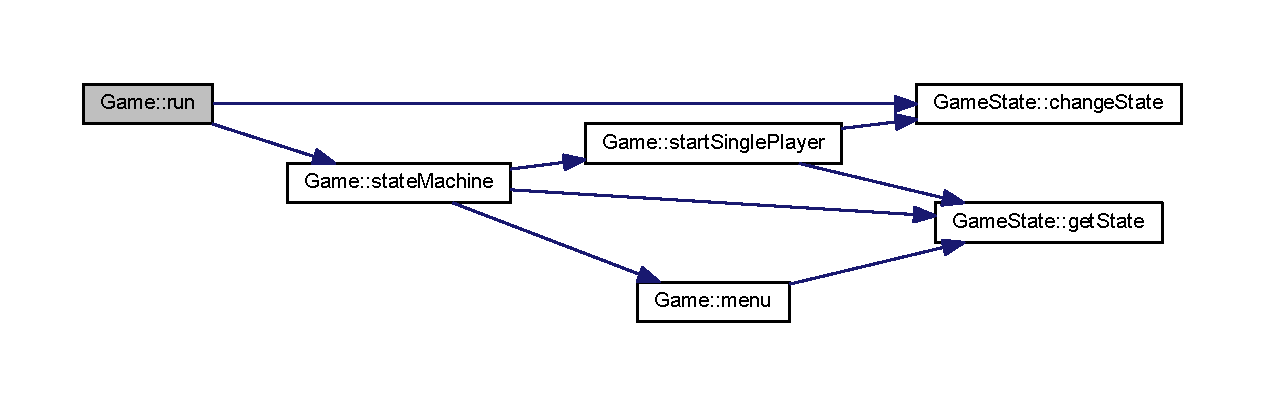
\includegraphics[width=350pt]{class_game_a1ab78f5ed0d5ea879157357cf2fb2afa_cgraph}
\end{center}
\end{figure}




Here is the caller graph for this function\+:\nopagebreak
\begin{figure}[H]
\begin{center}
\leavevmode
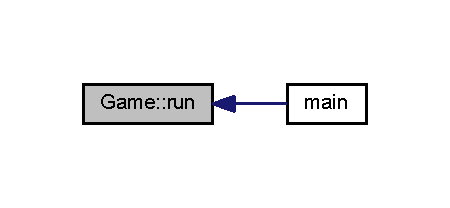
\includegraphics[width=216pt]{class_game_a1ab78f5ed0d5ea879157357cf2fb2afa_icgraph}
\end{center}
\end{figure}


\hypertarget{class_game_afbc524f7661c9ce1bea6ca45fd212093}{}\index{Game@{Game}!start\+Single\+Player@{start\+Single\+Player}}
\index{start\+Single\+Player@{start\+Single\+Player}!Game@{Game}}
\subsubsection[{start\+Single\+Player}]{\setlength{\rightskip}{0pt plus 5cm}void Game\+::start\+Single\+Player (
\begin{DoxyParamCaption}
{}
\end{DoxyParamCaption}
)}\label{class_game_afbc524f7661c9ce1bea6ca45fd212093}


Here is the caller graph for this function\+:\nopagebreak
\begin{figure}[H]
\begin{center}
\leavevmode
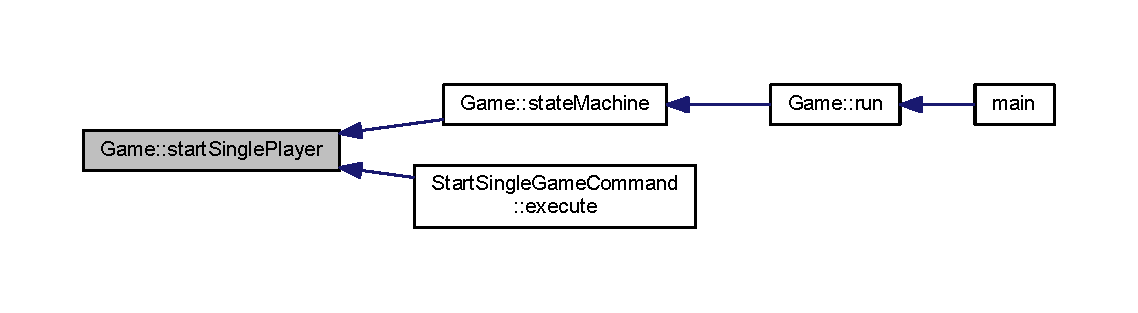
\includegraphics[width=350pt]{class_game_afbc524f7661c9ce1bea6ca45fd212093_icgraph}
\end{center}
\end{figure}


\hypertarget{class_game_a8bc94200bfbf0421b83b7c2b2b45da72}{}\index{Game@{Game}!state\+Machine@{state\+Machine}}
\index{state\+Machine@{state\+Machine}!Game@{Game}}
\subsubsection[{state\+Machine}]{\setlength{\rightskip}{0pt plus 5cm}void Game\+::state\+Machine (
\begin{DoxyParamCaption}
{}
\end{DoxyParamCaption}
)\hspace{0.3cm}{\ttfamily [private]}}\label{class_game_a8bc94200bfbf0421b83b7c2b2b45da72}


Here is the call graph for this function\+:\nopagebreak
\begin{figure}[H]
\begin{center}
\leavevmode
\includegraphics[width=346pt]{class_game_a8bc94200bfbf0421b83b7c2b2b45da72_cgraph}
\end{center}
\end{figure}




Here is the caller graph for this function\+:\nopagebreak
\begin{figure}[H]
\begin{center}
\leavevmode
\includegraphics[width=350pt]{class_game_a8bc94200bfbf0421b83b7c2b2b45da72_icgraph}
\end{center}
\end{figure}




\subsection{Member Data Documentation}
\hypertarget{class_game_aee6b9ebe224001f736e1ed71a3b28223}{}\index{Game@{Game}!engine@{engine}}
\index{engine@{engine}!Game@{Game}}
\subsubsection[{engine}]{\setlength{\rightskip}{0pt plus 5cm}std\+::unique\+\_\+ptr$<${\bf Engine}$>$ Game\+::engine}\label{class_game_aee6b9ebe224001f736e1ed71a3b28223}
\hypertarget{class_game_ae08cf171b4f973d47def68d69f561e2c}{}\index{Game@{Game}!main\+\_\+menu@{main\+\_\+menu}}
\index{main\+\_\+menu@{main\+\_\+menu}!Game@{Game}}
\subsubsection[{main\+\_\+menu}]{\setlength{\rightskip}{0pt plus 5cm}std\+::unique\+\_\+ptr$<${\bf Menu}$>$ Game\+::main\+\_\+menu}\label{class_game_ae08cf171b4f973d47def68d69f561e2c}
\hypertarget{class_game_a82776f65732ac43cf35b8b7c7120c873}{}\index{Game@{Game}!menu\+\_\+input@{menu\+\_\+input}}
\index{menu\+\_\+input@{menu\+\_\+input}!Game@{Game}}
\subsubsection[{menu\+\_\+input}]{\setlength{\rightskip}{0pt plus 5cm}std\+::unique\+\_\+ptr$<${\bf Input\+Handler}$>$ Game\+::menu\+\_\+input\hspace{0.3cm}{\ttfamily [private]}}\label{class_game_a82776f65732ac43cf35b8b7c7120c873}
\hypertarget{class_game_ad9fc2a8710ee56916f79314b91112ed0}{}\index{Game@{Game}!state@{state}}
\index{state@{state}!Game@{Game}}
\subsubsection[{state}]{\setlength{\rightskip}{0pt plus 5cm}{\bf Game\+State} Game\+::state\hspace{0.3cm}{\ttfamily [private]}}\label{class_game_ad9fc2a8710ee56916f79314b91112ed0}
\hypertarget{class_game_ad0fb4d8653dcf289fd6573cf5ba0f3d1}{}\index{Game@{Game}!window@{window}}
\index{window@{window}!Game@{Game}}
\subsubsection[{window}]{\setlength{\rightskip}{0pt plus 5cm}sf\+::\+Render\+Window\& Game\+::window\hspace{0.3cm}{\ttfamily [private]}}\label{class_game_ad0fb4d8653dcf289fd6573cf5ba0f3d1}


Main game window. 



The documentation for this class was generated from the following files\+:\begin{DoxyCompactItemize}
\item 
\hyperlink{_game_8h}{Game.\+h}\item 
\hyperlink{_game_8cpp}{Game.\+cpp}\end{DoxyCompactItemize}

\hypertarget{class_game_object}{}\section{Game\+Object Class Reference}
\label{class_game_object}\index{Game\+Object@{Game\+Object}}


{\ttfamily \#include $<$Game\+Object.\+h$>$}



Inheritance diagram for Game\+Object\+:\nopagebreak
\begin{figure}[H]
\begin{center}
\leavevmode
\includegraphics[width=350pt]{class_game_object__inherit__graph}
\end{center}
\end{figure}


Collaboration diagram for Game\+Object\+:\nopagebreak
\begin{figure}[H]
\begin{center}
\leavevmode
\includegraphics[width=172pt]{class_game_object__coll__graph}
\end{center}
\end{figure}
\subsection*{Public Member Functions}
\begin{DoxyCompactItemize}
\item 
\hyperlink{class_game_object_a0348e3ee2e83d56eafca7a3547f432c4}{Game\+Object} ()
\item 
virtual \hyperlink{class_game_object_ab82dfdb656f9051c0587e6593b2dda97}{$\sim$\+Game\+Object} ()
\item 
virtual void \hyperlink{class_game_object_a370e89c4bb00a8fb851d9279480f7f76}{move} (const sf\+::\+Vector2f \&offset)=0
\item 
virtual const sf\+::\+Vector2f \& \hyperlink{class_game_object_aba7c07744a79defec4484fb09d917543}{get\+Position} () const =0
\item 
virtual void \hyperlink{class_game_object_ad4a07f19f6c5e2e71c89c07486f26244}{update} ()
\item 
virtual void \hyperlink{class_game_object_a07a0da194460f2642732f45d7ad369e8}{render} (sf\+::\+Render\+Window \&window)=0
\end{DoxyCompactItemize}
\subsection*{Public Attributes}
\begin{DoxyCompactItemize}
\item 
sf\+::\+Vector2f \hyperlink{class_game_object_a485ee182e36f89f5493801bdd3c88d4a}{speed}
\item 
sf\+::\+Vector2f \hyperlink{class_game_object_a852964d6b689b4e12cc399fc67f4f8bf}{acceleration}
\end{DoxyCompactItemize}


\subsection{Constructor \& Destructor Documentation}
\hypertarget{class_game_object_a0348e3ee2e83d56eafca7a3547f432c4}{}\index{Game\+Object@{Game\+Object}!Game\+Object@{Game\+Object}}
\index{Game\+Object@{Game\+Object}!Game\+Object@{Game\+Object}}
\subsubsection[{Game\+Object}]{\setlength{\rightskip}{0pt plus 5cm}Game\+Object\+::\+Game\+Object (
\begin{DoxyParamCaption}
{}
\end{DoxyParamCaption}
)}\label{class_game_object_a0348e3ee2e83d56eafca7a3547f432c4}
\hypertarget{class_game_object_ab82dfdb656f9051c0587e6593b2dda97}{}\index{Game\+Object@{Game\+Object}!````~Game\+Object@{$\sim$\+Game\+Object}}
\index{````~Game\+Object@{$\sim$\+Game\+Object}!Game\+Object@{Game\+Object}}
\subsubsection[{$\sim$\+Game\+Object}]{\setlength{\rightskip}{0pt plus 5cm}Game\+Object\+::$\sim$\+Game\+Object (
\begin{DoxyParamCaption}
{}
\end{DoxyParamCaption}
)\hspace{0.3cm}{\ttfamily [virtual]}}\label{class_game_object_ab82dfdb656f9051c0587e6593b2dda97}


\subsection{Member Function Documentation}
\hypertarget{class_game_object_aba7c07744a79defec4484fb09d917543}{}\index{Game\+Object@{Game\+Object}!get\+Position@{get\+Position}}
\index{get\+Position@{get\+Position}!Game\+Object@{Game\+Object}}
\subsubsection[{get\+Position}]{\setlength{\rightskip}{0pt plus 5cm}virtual const sf\+::\+Vector2f\& Game\+Object\+::get\+Position (
\begin{DoxyParamCaption}
{}
\end{DoxyParamCaption}
) const\hspace{0.3cm}{\ttfamily [pure virtual]}}\label{class_game_object_aba7c07744a79defec4484fb09d917543}


Implemented in \hyperlink{class_enemy_ade0ec5d0a52a35a387a4cdcccf4c9ddc}{Enemy}, \hyperlink{class_player_abbd4bab9c1c4f881b268b37c3f810bd0}{Player}, and \hyperlink{class_bullet_a405c853cbdaffd53d506eb3ee474a3ef}{Bullet}.



Here is the caller graph for this function\+:\nopagebreak
\begin{figure}[H]
\begin{center}
\leavevmode
\includegraphics[width=350pt]{class_game_object_aba7c07744a79defec4484fb09d917543_icgraph}
\end{center}
\end{figure}


\hypertarget{class_game_object_a370e89c4bb00a8fb851d9279480f7f76}{}\index{Game\+Object@{Game\+Object}!move@{move}}
\index{move@{move}!Game\+Object@{Game\+Object}}
\subsubsection[{move}]{\setlength{\rightskip}{0pt plus 5cm}virtual void Game\+Object\+::move (
\begin{DoxyParamCaption}
\item[{const sf\+::\+Vector2f \&}]{offset}
\end{DoxyParamCaption}
)\hspace{0.3cm}{\ttfamily [pure virtual]}}\label{class_game_object_a370e89c4bb00a8fb851d9279480f7f76}


Implemented in \hyperlink{class_bullet_a8715ab2edff76c8b45fabc6dc453e85d}{Bullet}, \hyperlink{class_player_a0512220b727eb0cdc6e7d7141b13c7fd}{Player}, and \hyperlink{class_enemy_a4db256c45aa8d835561e035969883069}{Enemy}.



Here is the caller graph for this function\+:\nopagebreak
\begin{figure}[H]
\begin{center}
\leavevmode
\includegraphics[width=350pt]{class_game_object_a370e89c4bb00a8fb851d9279480f7f76_icgraph}
\end{center}
\end{figure}


\hypertarget{class_game_object_a07a0da194460f2642732f45d7ad369e8}{}\index{Game\+Object@{Game\+Object}!render@{render}}
\index{render@{render}!Game\+Object@{Game\+Object}}
\subsubsection[{render}]{\setlength{\rightskip}{0pt plus 5cm}virtual void Game\+Object\+::render (
\begin{DoxyParamCaption}
\item[{sf\+::\+Render\+Window \&}]{window}
\end{DoxyParamCaption}
)\hspace{0.3cm}{\ttfamily [pure virtual]}}\label{class_game_object_a07a0da194460f2642732f45d7ad369e8}


Implemented in \hyperlink{class_enemy_a409d7d48e2f6bb27f878691f14a79957}{Enemy}, \hyperlink{class_player_a53938857e80374e79726309e78d1c15c}{Player}, and \hyperlink{class_bullet_ae4af350647e1b2a798eb3fd35a883b84}{Bullet}.

\hypertarget{class_game_object_ad4a07f19f6c5e2e71c89c07486f26244}{}\index{Game\+Object@{Game\+Object}!update@{update}}
\index{update@{update}!Game\+Object@{Game\+Object}}
\subsubsection[{update}]{\setlength{\rightskip}{0pt plus 5cm}virtual void Game\+Object\+::update (
\begin{DoxyParamCaption}
{}
\end{DoxyParamCaption}
)\hspace{0.3cm}{\ttfamily [inline]}, {\ttfamily [virtual]}}\label{class_game_object_ad4a07f19f6c5e2e71c89c07486f26244}


Reimplemented in \hyperlink{class_enemy_aa70d742da02995011f1618acc9e303db}{Enemy}, and \hyperlink{class_player_a82c3476f3e65a4e2ac6bcd040771bdd4}{Player}.



Here is the call graph for this function\+:\nopagebreak
\begin{figure}[H]
\begin{center}
\leavevmode
\includegraphics[width=323pt]{class_game_object_ad4a07f19f6c5e2e71c89c07486f26244_cgraph}
\end{center}
\end{figure}




Here is the caller graph for this function\+:\nopagebreak
\begin{figure}[H]
\begin{center}
\leavevmode
\includegraphics[width=350pt]{class_game_object_ad4a07f19f6c5e2e71c89c07486f26244_icgraph}
\end{center}
\end{figure}




\subsection{Member Data Documentation}
\hypertarget{class_game_object_a852964d6b689b4e12cc399fc67f4f8bf}{}\index{Game\+Object@{Game\+Object}!acceleration@{acceleration}}
\index{acceleration@{acceleration}!Game\+Object@{Game\+Object}}
\subsubsection[{acceleration}]{\setlength{\rightskip}{0pt plus 5cm}sf\+::\+Vector2f Game\+Object\+::acceleration}\label{class_game_object_a852964d6b689b4e12cc399fc67f4f8bf}
\hypertarget{class_game_object_a485ee182e36f89f5493801bdd3c88d4a}{}\index{Game\+Object@{Game\+Object}!speed@{speed}}
\index{speed@{speed}!Game\+Object@{Game\+Object}}
\subsubsection[{speed}]{\setlength{\rightskip}{0pt plus 5cm}sf\+::\+Vector2f Game\+Object\+::speed}\label{class_game_object_a485ee182e36f89f5493801bdd3c88d4a}


The documentation for this class was generated from the following files\+:\begin{DoxyCompactItemize}
\item 
\hyperlink{_game_object_8h}{Game\+Object.\+h}\item 
\hyperlink{_game_object_8cpp}{Game\+Object.\+cpp}\end{DoxyCompactItemize}

\hypertarget{class_input_handler}{}\section{Input\+Handler Class Reference}
\label{class_input_handler}\index{Input\+Handler@{Input\+Handler}}


{\ttfamily \#include $<$Input\+Handler.\+h$>$}



Inheritance diagram for Input\+Handler\+:
\nopagebreak
\begin{figure}[H]
\begin{center}
\leavevmode
\includegraphics[width=350pt]{class_input_handler__inherit__graph}
\end{center}
\end{figure}


Collaboration diagram for Input\+Handler\+:\nopagebreak
\begin{figure}[H]
\begin{center}
\leavevmode
\includegraphics[width=210pt]{class_input_handler__coll__graph}
\end{center}
\end{figure}
\subsection*{Public Member Functions}
\begin{DoxyCompactItemize}
\item 
\hyperlink{class_input_handler_a1b1ccf055510e8ae1fc6a4a1d1fadbe4}{Input\+Handler} (int size)
\item 
virtual \hyperlink{class_input_handler_ac1f7efb54b34d433d6ffba62627452b6}{$\sim$\+Input\+Handler} ()
\item 
virtual \hyperlink{class_command}{Command} $\ast$$\ast$ \hyperlink{class_input_handler_a69b726d4a409a6f4ae443689cb69b404}{handle\+Input} ()=0
\end{DoxyCompactItemize}
\subsection*{Protected Attributes}
\begin{DoxyCompactItemize}
\item 
std\+::unique\+\_\+ptr$<$ \hyperlink{class_command}{Command} $\ast$\mbox{[}$\,$\mbox{]}$>$ \hyperlink{class_input_handler_abdd9f29f8c4b193f16679eddd05bdebd}{current\+\_\+command\+\_\+array}
\end{DoxyCompactItemize}


\subsection{Constructor \& Destructor Documentation}
\hypertarget{class_input_handler_a1b1ccf055510e8ae1fc6a4a1d1fadbe4}{}\index{Input\+Handler@{Input\+Handler}!Input\+Handler@{Input\+Handler}}
\index{Input\+Handler@{Input\+Handler}!Input\+Handler@{Input\+Handler}}
\subsubsection[{Input\+Handler}]{\setlength{\rightskip}{0pt plus 5cm}Input\+Handler\+::\+Input\+Handler (
\begin{DoxyParamCaption}
\item[{int}]{size}
\end{DoxyParamCaption}
)}\label{class_input_handler_a1b1ccf055510e8ae1fc6a4a1d1fadbe4}
\hypertarget{class_input_handler_ac1f7efb54b34d433d6ffba62627452b6}{}\index{Input\+Handler@{Input\+Handler}!````~Input\+Handler@{$\sim$\+Input\+Handler}}
\index{````~Input\+Handler@{$\sim$\+Input\+Handler}!Input\+Handler@{Input\+Handler}}
\subsubsection[{$\sim$\+Input\+Handler}]{\setlength{\rightskip}{0pt plus 5cm}Input\+Handler\+::$\sim$\+Input\+Handler (
\begin{DoxyParamCaption}
{}
\end{DoxyParamCaption}
)\hspace{0.3cm}{\ttfamily [virtual]}}\label{class_input_handler_ac1f7efb54b34d433d6ffba62627452b6}


\subsection{Member Function Documentation}
\hypertarget{class_input_handler_a69b726d4a409a6f4ae443689cb69b404}{}\index{Input\+Handler@{Input\+Handler}!handle\+Input@{handle\+Input}}
\index{handle\+Input@{handle\+Input}!Input\+Handler@{Input\+Handler}}
\subsubsection[{handle\+Input}]{\setlength{\rightskip}{0pt plus 5cm}virtual {\bf Command}$\ast$$\ast$ Input\+Handler\+::handle\+Input (
\begin{DoxyParamCaption}
{}
\end{DoxyParamCaption}
)\hspace{0.3cm}{\ttfamily [pure virtual]}}\label{class_input_handler_a69b726d4a409a6f4ae443689cb69b404}


Implemented in \hyperlink{class_ai_controler_a72891536d5ff122ae1e3a25fd62fd1b5}{Ai\+Controler}, \hyperlink{class_menu_input_handler_a60840342f557c79f31097aa713ba7a37}{Menu\+Input\+Handler}, \hyperlink{class_engine_input_handler_ade92afaf7657007c2be3b5bd745c96e3}{Engine\+Input\+Handler}, and \hyperlink{class_collision_handler_a7f6deb84dcebcc72e0020eb251ea617f}{Collision\+Handler}.



\subsection{Member Data Documentation}
\hypertarget{class_input_handler_abdd9f29f8c4b193f16679eddd05bdebd}{}\index{Input\+Handler@{Input\+Handler}!current\+\_\+command\+\_\+array@{current\+\_\+command\+\_\+array}}
\index{current\+\_\+command\+\_\+array@{current\+\_\+command\+\_\+array}!Input\+Handler@{Input\+Handler}}
\subsubsection[{current\+\_\+command\+\_\+array}]{\setlength{\rightskip}{0pt plus 5cm}std\+::unique\+\_\+ptr$<${\bf Command}$\ast$\mbox{[}$\,$\mbox{]}$>$ Input\+Handler\+::current\+\_\+command\+\_\+array\hspace{0.3cm}{\ttfamily [protected]}}\label{class_input_handler_abdd9f29f8c4b193f16679eddd05bdebd}


The documentation for this class was generated from the following files\+:\begin{DoxyCompactItemize}
\item 
\hyperlink{_input_handler_8h}{Input\+Handler.\+h}\item 
\hyperlink{_input_handler_8cpp}{Input\+Handler.\+cpp}\end{DoxyCompactItemize}

\hypertarget{class_main_menu}{}\section{Main\+Menu Class Reference}
\label{class_main_menu}\index{Main\+Menu@{Main\+Menu}}


{\ttfamily \#include $<$Main\+Menu.\+h$>$}



Inheritance diagram for Main\+Menu\+:\nopagebreak
\begin{figure}[H]
\begin{center}
\leavevmode
\includegraphics[width=248pt]{class_main_menu__inherit__graph}
\end{center}
\end{figure}


Collaboration diagram for Main\+Menu\+:\nopagebreak
\begin{figure}[H]
\begin{center}
\leavevmode
\includegraphics[width=248pt]{class_main_menu__coll__graph}
\end{center}
\end{figure}
\subsection*{Public Member Functions}
\begin{DoxyCompactItemize}
\item 
int \hyperlink{class_main_menu_aec279c06705f829ab154b9023ec838b3}{get\+Number\+Of\+Menu\+Choices} () override
\item 
void \hyperlink{class_main_menu_a1487a843dd8cf56374afa60a5b62e9bf}{render} (sf\+::\+Render\+Window \&window) override
\item 
\hyperlink{class_main_menu_a53eecf9d5ffd094f54ac4193e7e57eaf}{Main\+Menu} ()
\item 
virtual \hyperlink{class_main_menu_a0a19ddba3ac52bf39c09b579171c98f2}{$\sim$\+Main\+Menu} ()
\item 
sf\+::\+Text $\ast$\& \hyperlink{class_main_menu_abdf7a2a5bca4e2916bf9dc218c0de96f}{get\+Selected\+Text\+Ptr} () override
\item 
sf\+::\+Text \& \hyperlink{class_main_menu_ac5be2a5b81d51c79dfeab061263e00ba}{get\+Menu\+Text} (int i) override
\end{DoxyCompactItemize}
\subsection*{Protected Attributes}
\begin{DoxyCompactItemize}
\item 
const int \hyperlink{class_main_menu_a22354cddce5d5cc36bfa1dbc5eb951fa}{N\+U\+M\+B\+E\+R\+\_\+\+O\+F\+\_\+\+M\+E\+N\+U\+\_\+\+C\+H\+O\+I\+C\+E\+S}
\item 
std\+::unique\+\_\+ptr$<$ sf\+::\+Text\mbox{[}$\,$\mbox{]}$>$ \hyperlink{class_main_menu_a95c0a8c6a4fab313fa4706f4d407413d}{menu\+\_\+text}
\item 
sf\+::\+Font \hyperlink{class_main_menu_a77e075ce7fa6f3331cf82187ec54da88}{font}
\item 
sf\+::\+Text $\ast$ \hyperlink{class_main_menu_a0a0ebee9f052974eb46c411f1dbaa2fc}{selected\+\_\+text}
\end{DoxyCompactItemize}


\subsection{Constructor \& Destructor Documentation}
\hypertarget{class_main_menu_a53eecf9d5ffd094f54ac4193e7e57eaf}{}\index{Main\+Menu@{Main\+Menu}!Main\+Menu@{Main\+Menu}}
\index{Main\+Menu@{Main\+Menu}!Main\+Menu@{Main\+Menu}}
\subsubsection[{Main\+Menu}]{\setlength{\rightskip}{0pt plus 5cm}Main\+Menu\+::\+Main\+Menu (
\begin{DoxyParamCaption}
{}
\end{DoxyParamCaption}
)}\label{class_main_menu_a53eecf9d5ffd094f54ac4193e7e57eaf}
\hypertarget{class_main_menu_a0a19ddba3ac52bf39c09b579171c98f2}{}\index{Main\+Menu@{Main\+Menu}!````~Main\+Menu@{$\sim$\+Main\+Menu}}
\index{````~Main\+Menu@{$\sim$\+Main\+Menu}!Main\+Menu@{Main\+Menu}}
\subsubsection[{$\sim$\+Main\+Menu}]{\setlength{\rightskip}{0pt plus 5cm}Main\+Menu\+::$\sim$\+Main\+Menu (
\begin{DoxyParamCaption}
{}
\end{DoxyParamCaption}
)\hspace{0.3cm}{\ttfamily [virtual]}}\label{class_main_menu_a0a19ddba3ac52bf39c09b579171c98f2}


\subsection{Member Function Documentation}
\hypertarget{class_main_menu_ac5be2a5b81d51c79dfeab061263e00ba}{}\index{Main\+Menu@{Main\+Menu}!get\+Menu\+Text@{get\+Menu\+Text}}
\index{get\+Menu\+Text@{get\+Menu\+Text}!Main\+Menu@{Main\+Menu}}
\subsubsection[{get\+Menu\+Text}]{\setlength{\rightskip}{0pt plus 5cm}sf\+::\+Text \& Main\+Menu\+::get\+Menu\+Text (
\begin{DoxyParamCaption}
\item[{int}]{i}
\end{DoxyParamCaption}
)\hspace{0.3cm}{\ttfamily [override]}, {\ttfamily [virtual]}}\label{class_main_menu_ac5be2a5b81d51c79dfeab061263e00ba}


Implements \hyperlink{class_menu_a42fb94aee459f7ae5d06a7be1b540f17}{Menu}.

\hypertarget{class_main_menu_aec279c06705f829ab154b9023ec838b3}{}\index{Main\+Menu@{Main\+Menu}!get\+Number\+Of\+Menu\+Choices@{get\+Number\+Of\+Menu\+Choices}}
\index{get\+Number\+Of\+Menu\+Choices@{get\+Number\+Of\+Menu\+Choices}!Main\+Menu@{Main\+Menu}}
\subsubsection[{get\+Number\+Of\+Menu\+Choices}]{\setlength{\rightskip}{0pt plus 5cm}int Main\+Menu\+::get\+Number\+Of\+Menu\+Choices (
\begin{DoxyParamCaption}
{}
\end{DoxyParamCaption}
)\hspace{0.3cm}{\ttfamily [override]}, {\ttfamily [virtual]}}\label{class_main_menu_aec279c06705f829ab154b9023ec838b3}


Implements \hyperlink{class_menu_aeed33b0a47d0c49de45e0c1bb1503585}{Menu}.

\hypertarget{class_main_menu_abdf7a2a5bca4e2916bf9dc218c0de96f}{}\index{Main\+Menu@{Main\+Menu}!get\+Selected\+Text\+Ptr@{get\+Selected\+Text\+Ptr}}
\index{get\+Selected\+Text\+Ptr@{get\+Selected\+Text\+Ptr}!Main\+Menu@{Main\+Menu}}
\subsubsection[{get\+Selected\+Text\+Ptr}]{\setlength{\rightskip}{0pt plus 5cm}sf\+::\+Text $\ast$\& Main\+Menu\+::get\+Selected\+Text\+Ptr (
\begin{DoxyParamCaption}
{}
\end{DoxyParamCaption}
)\hspace{0.3cm}{\ttfamily [override]}, {\ttfamily [virtual]}}\label{class_main_menu_abdf7a2a5bca4e2916bf9dc218c0de96f}


Implements \hyperlink{class_menu_ac9a761729ba9bac25bae4ee1a25b6e11}{Menu}.

\hypertarget{class_main_menu_a1487a843dd8cf56374afa60a5b62e9bf}{}\index{Main\+Menu@{Main\+Menu}!render@{render}}
\index{render@{render}!Main\+Menu@{Main\+Menu}}
\subsubsection[{render}]{\setlength{\rightskip}{0pt plus 5cm}void Main\+Menu\+::render (
\begin{DoxyParamCaption}
\item[{sf\+::\+Render\+Window \&}]{window}
\end{DoxyParamCaption}
)\hspace{0.3cm}{\ttfamily [override]}, {\ttfamily [virtual]}}\label{class_main_menu_a1487a843dd8cf56374afa60a5b62e9bf}


Implements \hyperlink{class_menu_aa2297a6abfaa404403fe1b7ae2521f88}{Menu}.



\subsection{Member Data Documentation}
\hypertarget{class_main_menu_a77e075ce7fa6f3331cf82187ec54da88}{}\index{Main\+Menu@{Main\+Menu}!font@{font}}
\index{font@{font}!Main\+Menu@{Main\+Menu}}
\subsubsection[{font}]{\setlength{\rightskip}{0pt plus 5cm}sf\+::\+Font Main\+Menu\+::font\hspace{0.3cm}{\ttfamily [protected]}}\label{class_main_menu_a77e075ce7fa6f3331cf82187ec54da88}
\hypertarget{class_main_menu_a95c0a8c6a4fab313fa4706f4d407413d}{}\index{Main\+Menu@{Main\+Menu}!menu\+\_\+text@{menu\+\_\+text}}
\index{menu\+\_\+text@{menu\+\_\+text}!Main\+Menu@{Main\+Menu}}
\subsubsection[{menu\+\_\+text}]{\setlength{\rightskip}{0pt plus 5cm}std\+::unique\+\_\+ptr$<$sf\+::\+Text\mbox{[}$\,$\mbox{]}$>$ Main\+Menu\+::menu\+\_\+text\hspace{0.3cm}{\ttfamily [protected]}}\label{class_main_menu_a95c0a8c6a4fab313fa4706f4d407413d}
\hypertarget{class_main_menu_a22354cddce5d5cc36bfa1dbc5eb951fa}{}\index{Main\+Menu@{Main\+Menu}!N\+U\+M\+B\+E\+R\+\_\+\+O\+F\+\_\+\+M\+E\+N\+U\+\_\+\+C\+H\+O\+I\+C\+E\+S@{N\+U\+M\+B\+E\+R\+\_\+\+O\+F\+\_\+\+M\+E\+N\+U\+\_\+\+C\+H\+O\+I\+C\+E\+S}}
\index{N\+U\+M\+B\+E\+R\+\_\+\+O\+F\+\_\+\+M\+E\+N\+U\+\_\+\+C\+H\+O\+I\+C\+E\+S@{N\+U\+M\+B\+E\+R\+\_\+\+O\+F\+\_\+\+M\+E\+N\+U\+\_\+\+C\+H\+O\+I\+C\+E\+S}!Main\+Menu@{Main\+Menu}}
\subsubsection[{N\+U\+M\+B\+E\+R\+\_\+\+O\+F\+\_\+\+M\+E\+N\+U\+\_\+\+C\+H\+O\+I\+C\+E\+S}]{\setlength{\rightskip}{0pt plus 5cm}const int Main\+Menu\+::\+N\+U\+M\+B\+E\+R\+\_\+\+O\+F\+\_\+\+M\+E\+N\+U\+\_\+\+C\+H\+O\+I\+C\+E\+S\hspace{0.3cm}{\ttfamily [protected]}}\label{class_main_menu_a22354cddce5d5cc36bfa1dbc5eb951fa}
\hypertarget{class_main_menu_a0a0ebee9f052974eb46c411f1dbaa2fc}{}\index{Main\+Menu@{Main\+Menu}!selected\+\_\+text@{selected\+\_\+text}}
\index{selected\+\_\+text@{selected\+\_\+text}!Main\+Menu@{Main\+Menu}}
\subsubsection[{selected\+\_\+text}]{\setlength{\rightskip}{0pt plus 5cm}sf\+::\+Text$\ast$ Main\+Menu\+::selected\+\_\+text\hspace{0.3cm}{\ttfamily [protected]}}\label{class_main_menu_a0a0ebee9f052974eb46c411f1dbaa2fc}


The documentation for this class was generated from the following files\+:\begin{DoxyCompactItemize}
\item 
\hyperlink{_main_menu_8h}{Main\+Menu.\+h}\item 
\hyperlink{_main_menu_8cpp}{Main\+Menu.\+cpp}\end{DoxyCompactItemize}

\hypertarget{class_menu}{}\section{Menu Class Reference}
\label{class_menu}\index{Menu@{Menu}}


{\ttfamily \#include $<$Menu.\+h$>$}



Inheritance diagram for Menu\+:\nopagebreak
\begin{figure}[H]
\begin{center}
\leavevmode
\includegraphics[width=248pt]{class_menu__inherit__graph}
\end{center}
\end{figure}


Collaboration diagram for Menu\+:\nopagebreak
\begin{figure}[H]
\begin{center}
\leavevmode
\includegraphics[width=228pt]{class_menu__coll__graph}
\end{center}
\end{figure}
\subsection*{Public Member Functions}
\begin{DoxyCompactItemize}
\item 
virtual void \hyperlink{class_menu_aa2297a6abfaa404403fe1b7ae2521f88}{render} (sf\+::\+Render\+Window \&window)=0
\item 
virtual int \hyperlink{class_menu_aeed33b0a47d0c49de45e0c1bb1503585}{get\+Number\+Of\+Menu\+Choices} ()=0
\item 
virtual \hyperlink{class_menu_a831387f51358cfb88cd018e1777bc980}{$\sim$\+Menu} ()
\item 
virtual sf\+::\+Text $\ast$\& \hyperlink{class_menu_ac9a761729ba9bac25bae4ee1a25b6e11}{get\+Selected\+Text\+Ptr} ()=0
\item 
virtual sf\+::\+Text \& \hyperlink{class_menu_a42fb94aee459f7ae5d06a7be1b540f17}{get\+Menu\+Text} (int i)=0
\end{DoxyCompactItemize}


\subsection{Constructor \& Destructor Documentation}
\hypertarget{class_menu_a831387f51358cfb88cd018e1777bc980}{}\index{Menu@{Menu}!````~Menu@{$\sim$\+Menu}}
\index{````~Menu@{$\sim$\+Menu}!Menu@{Menu}}
\subsubsection[{$\sim$\+Menu}]{\setlength{\rightskip}{0pt plus 5cm}Menu\+::$\sim$\+Menu (
\begin{DoxyParamCaption}
{}
\end{DoxyParamCaption}
)\hspace{0.3cm}{\ttfamily [virtual]}}\label{class_menu_a831387f51358cfb88cd018e1777bc980}


\subsection{Member Function Documentation}
\hypertarget{class_menu_a42fb94aee459f7ae5d06a7be1b540f17}{}\index{Menu@{Menu}!get\+Menu\+Text@{get\+Menu\+Text}}
\index{get\+Menu\+Text@{get\+Menu\+Text}!Menu@{Menu}}
\subsubsection[{get\+Menu\+Text}]{\setlength{\rightskip}{0pt plus 5cm}virtual sf\+::\+Text\& Menu\+::get\+Menu\+Text (
\begin{DoxyParamCaption}
\item[{int}]{i}
\end{DoxyParamCaption}
)\hspace{0.3cm}{\ttfamily [pure virtual]}}\label{class_menu_a42fb94aee459f7ae5d06a7be1b540f17}


Implemented in \hyperlink{class_main_menu_ac5be2a5b81d51c79dfeab061263e00ba}{Main\+Menu}.



Here is the caller graph for this function\+:
\nopagebreak
\begin{figure}[H]
\begin{center}
\leavevmode
\includegraphics[width=350pt]{class_menu_a42fb94aee459f7ae5d06a7be1b540f17_icgraph}
\end{center}
\end{figure}


\hypertarget{class_menu_aeed33b0a47d0c49de45e0c1bb1503585}{}\index{Menu@{Menu}!get\+Number\+Of\+Menu\+Choices@{get\+Number\+Of\+Menu\+Choices}}
\index{get\+Number\+Of\+Menu\+Choices@{get\+Number\+Of\+Menu\+Choices}!Menu@{Menu}}
\subsubsection[{get\+Number\+Of\+Menu\+Choices}]{\setlength{\rightskip}{0pt plus 5cm}virtual int Menu\+::get\+Number\+Of\+Menu\+Choices (
\begin{DoxyParamCaption}
{}
\end{DoxyParamCaption}
)\hspace{0.3cm}{\ttfamily [pure virtual]}}\label{class_menu_aeed33b0a47d0c49de45e0c1bb1503585}


Implemented in \hyperlink{class_main_menu_aec279c06705f829ab154b9023ec838b3}{Main\+Menu}.



Here is the caller graph for this function\+:
\nopagebreak
\begin{figure}[H]
\begin{center}
\leavevmode
\includegraphics[width=350pt]{class_menu_aeed33b0a47d0c49de45e0c1bb1503585_icgraph}
\end{center}
\end{figure}


\hypertarget{class_menu_ac9a761729ba9bac25bae4ee1a25b6e11}{}\index{Menu@{Menu}!get\+Selected\+Text\+Ptr@{get\+Selected\+Text\+Ptr}}
\index{get\+Selected\+Text\+Ptr@{get\+Selected\+Text\+Ptr}!Menu@{Menu}}
\subsubsection[{get\+Selected\+Text\+Ptr}]{\setlength{\rightskip}{0pt plus 5cm}virtual sf\+::\+Text$\ast$\& Menu\+::get\+Selected\+Text\+Ptr (
\begin{DoxyParamCaption}
{}
\end{DoxyParamCaption}
)\hspace{0.3cm}{\ttfamily [pure virtual]}}\label{class_menu_ac9a761729ba9bac25bae4ee1a25b6e11}


Implemented in \hyperlink{class_main_menu_abdf7a2a5bca4e2916bf9dc218c0de96f}{Main\+Menu}.



Here is the caller graph for this function\+:
\nopagebreak
\begin{figure}[H]
\begin{center}
\leavevmode
\includegraphics[width=350pt]{class_menu_ac9a761729ba9bac25bae4ee1a25b6e11_icgraph}
\end{center}
\end{figure}


\hypertarget{class_menu_aa2297a6abfaa404403fe1b7ae2521f88}{}\index{Menu@{Menu}!render@{render}}
\index{render@{render}!Menu@{Menu}}
\subsubsection[{render}]{\setlength{\rightskip}{0pt plus 5cm}virtual void Menu\+::render (
\begin{DoxyParamCaption}
\item[{sf\+::\+Render\+Window \&}]{window}
\end{DoxyParamCaption}
)\hspace{0.3cm}{\ttfamily [pure virtual]}}\label{class_menu_aa2297a6abfaa404403fe1b7ae2521f88}


Implemented in \hyperlink{class_main_menu_a1487a843dd8cf56374afa60a5b62e9bf}{Main\+Menu}.



The documentation for this class was generated from the following files\+:\begin{DoxyCompactItemize}
\item 
\hyperlink{_menu_8h}{Menu.\+h}\item 
\hyperlink{_menu_8cpp}{Menu.\+cpp}\end{DoxyCompactItemize}

\hypertarget{class_menu_command}{}\section{Menu\+Command Class Reference}
\label{class_menu_command}\index{Menu\+Command@{Menu\+Command}}


{\ttfamily \#include $<$Menu\+Command.\+h$>$}



Inheritance diagram for Menu\+Command\+:
\nopagebreak
\begin{figure}[H]
\begin{center}
\leavevmode
\includegraphics[width=186pt]{class_menu_command__inherit__graph}
\end{center}
\end{figure}


Collaboration diagram for Menu\+Command\+:
\nopagebreak
\begin{figure}[H]
\begin{center}
\leavevmode
\includegraphics[width=186pt]{class_menu_command__coll__graph}
\end{center}
\end{figure}
\subsection*{Public Member Functions}
\begin{DoxyCompactItemize}
\item 
virtual void \hyperlink{class_menu_command_ac5d1ade9cec6d0540cb8e9ff0e84574c}{execute} ()=0
\item 
virtual \hyperlink{class_menu_command_a7b61310cfc662b7d37366dca0df75ca8}{$\sim$\+Menu\+Command} ()
\end{DoxyCompactItemize}
\subsection*{Additional Inherited Members}


\subsection{Constructor \& Destructor Documentation}
\hypertarget{class_menu_command_a7b61310cfc662b7d37366dca0df75ca8}{}\index{Menu\+Command@{Menu\+Command}!````~Menu\+Command@{$\sim$\+Menu\+Command}}
\index{````~Menu\+Command@{$\sim$\+Menu\+Command}!Menu\+Command@{Menu\+Command}}
\subsubsection[{$\sim$\+Menu\+Command}]{\setlength{\rightskip}{0pt plus 5cm}Menu\+Command\+::$\sim$\+Menu\+Command (
\begin{DoxyParamCaption}
{}
\end{DoxyParamCaption}
)\hspace{0.3cm}{\ttfamily [virtual]}}\label{class_menu_command_a7b61310cfc662b7d37366dca0df75ca8}


\subsection{Member Function Documentation}
\hypertarget{class_menu_command_ac5d1ade9cec6d0540cb8e9ff0e84574c}{}\index{Menu\+Command@{Menu\+Command}!execute@{execute}}
\index{execute@{execute}!Menu\+Command@{Menu\+Command}}
\subsubsection[{execute}]{\setlength{\rightskip}{0pt plus 5cm}void Menu\+Command\+::execute (
\begin{DoxyParamCaption}
{}
\end{DoxyParamCaption}
)\hspace{0.3cm}{\ttfamily [pure virtual]}}\label{class_menu_command_ac5d1ade9cec6d0540cb8e9ff0e84574c}


Implements \hyperlink{class_command_a6fd7d9bd8df8bfc881e4d6c7cd1878b7}{Command}.



The documentation for this class was generated from the following files\+:\begin{DoxyCompactItemize}
\item 
\hyperlink{_menu_command_8h}{Menu\+Command.\+h}\item 
\hyperlink{_menu_command_8cpp}{Menu\+Command.\+cpp}\end{DoxyCompactItemize}

\hypertarget{class_menu_input_handler}{}\section{Menu\+Input\+Handler Class Reference}
\label{class_menu_input_handler}\index{Menu\+Input\+Handler@{Menu\+Input\+Handler}}


{\ttfamily \#include $<$Menu\+Input\+Handler.\+h$>$}



Inheritance diagram for Menu\+Input\+Handler\+:
\nopagebreak
\begin{figure}[H]
\begin{center}
\leavevmode
\includegraphics[width=210pt]{class_menu_input_handler__inherit__graph}
\end{center}
\end{figure}


Collaboration diagram for Menu\+Input\+Handler\+:
\nopagebreak
\begin{figure}[H]
\begin{center}
\leavevmode
\includegraphics[width=350pt]{class_menu_input_handler__coll__graph}
\end{center}
\end{figure}
\subsection*{Public Member Functions}
\begin{DoxyCompactItemize}
\item 
\hyperlink{class_command}{Command} $\ast$$\ast$ \hyperlink{class_menu_input_handler_a60840342f557c79f31097aa713ba7a37}{handle\+Input} () override
\item 
\hyperlink{class_menu_input_handler_a244c829acc6ffe44795e44cb2980615b}{Menu\+Input\+Handler} (\hyperlink{class_game_state}{Game\+State} \&game\+\_\+state\+\_\+in, \hyperlink{class_menu}{Menu} $\ast$menu\+\_\+in, sf\+::\+Render\+Window \&window\+\_\+in)
\item 
virtual \hyperlink{class_menu_input_handler_aad61207bccc58ff8c688ffb265ca13db}{$\sim$\+Menu\+Input\+Handler} ()
\end{DoxyCompactItemize}
\subsection*{Private Member Functions}
\begin{DoxyCompactItemize}
\item 
\hyperlink{class_command}{Command} $\ast$ \hyperlink{class_menu_input_handler_aefd1edfd9f0d0770383c4977416de3bf}{handle\+Key\+Input} (sf\+::\+Event \&event, int \&i)
\end{DoxyCompactItemize}
\subsection*{Private Attributes}
\begin{DoxyCompactItemize}
\item 
\hyperlink{class_game_state}{Game\+State} \& \hyperlink{class_menu_input_handler_a6574e69d6344c10cb1dd53c6e2ffac26}{game\+\_\+state}
\item 
sf\+::\+Render\+Window \& \hyperlink{class_menu_input_handler_a2d53ce9f0554202b62c1640ef95e799b}{window}
\item 
\hyperlink{class_menu}{Menu} $\ast$ \hyperlink{class_menu_input_handler_adda8b05fe971a0ed749bb0037d3ba4bd}{menu}
\item 
std\+::shared\+\_\+ptr$<$ \hyperlink{class_command}{Command} $>$ \hyperlink{class_menu_input_handler_abf019bb1ca2f82975870e932e3cbd558}{key\+\_\+escape}
\item 
std\+::shared\+\_\+ptr$<$ \hyperlink{class_command}{Command} $>$ \hyperlink{class_menu_input_handler_a493334cca9bde4229be296ad44e3db9b}{closed}
\item 
std\+::shared\+\_\+ptr$<$ \hyperlink{class_command}{Command} $>$ \hyperlink{class_menu_input_handler_a29143574ca3b79dccb3a98260184968c}{key\+\_\+down}
\item 
std\+::shared\+\_\+ptr$<$ \hyperlink{class_command}{Command} $>$ \hyperlink{class_menu_input_handler_aa16ab7856da1bc4c6dea371e244939fb}{key\+\_\+s}
\item 
std\+::shared\+\_\+ptr$<$ \hyperlink{class_command}{Command} $>$ \hyperlink{class_menu_input_handler_ae1b3b9df835e3182dba3bbf1fd8b98aa}{key\+\_\+up}
\item 
std\+::shared\+\_\+ptr$<$ \hyperlink{class_command}{Command} $>$ \hyperlink{class_menu_input_handler_a052c981814cc918c88d17d7b4f0deb0e}{key\+\_\+w}
\item 
std\+::shared\+\_\+ptr$<$ \hyperlink{class_command}{Command} $>$ \hyperlink{class_menu_input_handler_a8f596f6b958c7007a3ccc44ac3d8666e}{key\+\_\+space}
\end{DoxyCompactItemize}
\subsection*{Additional Inherited Members}


\subsection{Constructor \& Destructor Documentation}
\hypertarget{class_menu_input_handler_a244c829acc6ffe44795e44cb2980615b}{}\index{Menu\+Input\+Handler@{Menu\+Input\+Handler}!Menu\+Input\+Handler@{Menu\+Input\+Handler}}
\index{Menu\+Input\+Handler@{Menu\+Input\+Handler}!Menu\+Input\+Handler@{Menu\+Input\+Handler}}
\subsubsection[{Menu\+Input\+Handler}]{\setlength{\rightskip}{0pt plus 5cm}Menu\+Input\+Handler\+::\+Menu\+Input\+Handler (
\begin{DoxyParamCaption}
\item[{{\bf Game\+State} \&}]{game\+\_\+state\+\_\+in, }
\item[{{\bf Menu} $\ast$}]{menu\+\_\+in, }
\item[{sf\+::\+Render\+Window \&}]{window\+\_\+in}
\end{DoxyParamCaption}
)}\label{class_menu_input_handler_a244c829acc6ffe44795e44cb2980615b}
\hypertarget{class_menu_input_handler_aad61207bccc58ff8c688ffb265ca13db}{}\index{Menu\+Input\+Handler@{Menu\+Input\+Handler}!````~Menu\+Input\+Handler@{$\sim$\+Menu\+Input\+Handler}}
\index{````~Menu\+Input\+Handler@{$\sim$\+Menu\+Input\+Handler}!Menu\+Input\+Handler@{Menu\+Input\+Handler}}
\subsubsection[{$\sim$\+Menu\+Input\+Handler}]{\setlength{\rightskip}{0pt plus 5cm}Menu\+Input\+Handler\+::$\sim$\+Menu\+Input\+Handler (
\begin{DoxyParamCaption}
{}
\end{DoxyParamCaption}
)\hspace{0.3cm}{\ttfamily [virtual]}}\label{class_menu_input_handler_aad61207bccc58ff8c688ffb265ca13db}


\subsection{Member Function Documentation}
\hypertarget{class_menu_input_handler_a60840342f557c79f31097aa713ba7a37}{}\index{Menu\+Input\+Handler@{Menu\+Input\+Handler}!handle\+Input@{handle\+Input}}
\index{handle\+Input@{handle\+Input}!Menu\+Input\+Handler@{Menu\+Input\+Handler}}
\subsubsection[{handle\+Input}]{\setlength{\rightskip}{0pt plus 5cm}{\bf Command} $\ast$$\ast$ Menu\+Input\+Handler\+::handle\+Input (
\begin{DoxyParamCaption}
{}
\end{DoxyParamCaption}
)\hspace{0.3cm}{\ttfamily [override]}, {\ttfamily [virtual]}}\label{class_menu_input_handler_a60840342f557c79f31097aa713ba7a37}


Implements \hyperlink{class_input_handler_a69b726d4a409a6f4ae443689cb69b404}{Input\+Handler}.



Here is the call graph for this function\+:
\nopagebreak
\begin{figure}[H]
\begin{center}
\leavevmode
\includegraphics[width=350pt]{class_menu_input_handler_a60840342f557c79f31097aa713ba7a37_cgraph}
\end{center}
\end{figure}


\hypertarget{class_menu_input_handler_aefd1edfd9f0d0770383c4977416de3bf}{}\index{Menu\+Input\+Handler@{Menu\+Input\+Handler}!handle\+Key\+Input@{handle\+Key\+Input}}
\index{handle\+Key\+Input@{handle\+Key\+Input}!Menu\+Input\+Handler@{Menu\+Input\+Handler}}
\subsubsection[{handle\+Key\+Input}]{\setlength{\rightskip}{0pt plus 5cm}{\bf Command} $\ast$ Menu\+Input\+Handler\+::handle\+Key\+Input (
\begin{DoxyParamCaption}
\item[{sf\+::\+Event \&}]{event, }
\item[{int \&}]{i}
\end{DoxyParamCaption}
)\hspace{0.3cm}{\ttfamily [private]}}\label{class_menu_input_handler_aefd1edfd9f0d0770383c4977416de3bf}


Here is the caller graph for this function\+:\nopagebreak
\begin{figure}[H]
\begin{center}
\leavevmode
\includegraphics[width=350pt]{class_menu_input_handler_aefd1edfd9f0d0770383c4977416de3bf_icgraph}
\end{center}
\end{figure}




\subsection{Member Data Documentation}
\hypertarget{class_menu_input_handler_a493334cca9bde4229be296ad44e3db9b}{}\index{Menu\+Input\+Handler@{Menu\+Input\+Handler}!closed@{closed}}
\index{closed@{closed}!Menu\+Input\+Handler@{Menu\+Input\+Handler}}
\subsubsection[{closed}]{\setlength{\rightskip}{0pt plus 5cm}std\+::shared\+\_\+ptr$<${\bf Command}$>$ Menu\+Input\+Handler\+::closed\hspace{0.3cm}{\ttfamily [private]}}\label{class_menu_input_handler_a493334cca9bde4229be296ad44e3db9b}
\hypertarget{class_menu_input_handler_a6574e69d6344c10cb1dd53c6e2ffac26}{}\index{Menu\+Input\+Handler@{Menu\+Input\+Handler}!game\+\_\+state@{game\+\_\+state}}
\index{game\+\_\+state@{game\+\_\+state}!Menu\+Input\+Handler@{Menu\+Input\+Handler}}
\subsubsection[{game\+\_\+state}]{\setlength{\rightskip}{0pt plus 5cm}{\bf Game\+State}\& Menu\+Input\+Handler\+::game\+\_\+state\hspace{0.3cm}{\ttfamily [private]}}\label{class_menu_input_handler_a6574e69d6344c10cb1dd53c6e2ffac26}
\hypertarget{class_menu_input_handler_a29143574ca3b79dccb3a98260184968c}{}\index{Menu\+Input\+Handler@{Menu\+Input\+Handler}!key\+\_\+down@{key\+\_\+down}}
\index{key\+\_\+down@{key\+\_\+down}!Menu\+Input\+Handler@{Menu\+Input\+Handler}}
\subsubsection[{key\+\_\+down}]{\setlength{\rightskip}{0pt plus 5cm}std\+::shared\+\_\+ptr$<${\bf Command}$>$ Menu\+Input\+Handler\+::key\+\_\+down\hspace{0.3cm}{\ttfamily [private]}}\label{class_menu_input_handler_a29143574ca3b79dccb3a98260184968c}
\hypertarget{class_menu_input_handler_abf019bb1ca2f82975870e932e3cbd558}{}\index{Menu\+Input\+Handler@{Menu\+Input\+Handler}!key\+\_\+escape@{key\+\_\+escape}}
\index{key\+\_\+escape@{key\+\_\+escape}!Menu\+Input\+Handler@{Menu\+Input\+Handler}}
\subsubsection[{key\+\_\+escape}]{\setlength{\rightskip}{0pt plus 5cm}std\+::shared\+\_\+ptr$<${\bf Command}$>$ Menu\+Input\+Handler\+::key\+\_\+escape\hspace{0.3cm}{\ttfamily [private]}}\label{class_menu_input_handler_abf019bb1ca2f82975870e932e3cbd558}
\hypertarget{class_menu_input_handler_aa16ab7856da1bc4c6dea371e244939fb}{}\index{Menu\+Input\+Handler@{Menu\+Input\+Handler}!key\+\_\+s@{key\+\_\+s}}
\index{key\+\_\+s@{key\+\_\+s}!Menu\+Input\+Handler@{Menu\+Input\+Handler}}
\subsubsection[{key\+\_\+s}]{\setlength{\rightskip}{0pt plus 5cm}std\+::shared\+\_\+ptr$<${\bf Command}$>$ Menu\+Input\+Handler\+::key\+\_\+s\hspace{0.3cm}{\ttfamily [private]}}\label{class_menu_input_handler_aa16ab7856da1bc4c6dea371e244939fb}
\hypertarget{class_menu_input_handler_a8f596f6b958c7007a3ccc44ac3d8666e}{}\index{Menu\+Input\+Handler@{Menu\+Input\+Handler}!key\+\_\+space@{key\+\_\+space}}
\index{key\+\_\+space@{key\+\_\+space}!Menu\+Input\+Handler@{Menu\+Input\+Handler}}
\subsubsection[{key\+\_\+space}]{\setlength{\rightskip}{0pt plus 5cm}std\+::shared\+\_\+ptr$<${\bf Command}$>$ Menu\+Input\+Handler\+::key\+\_\+space\hspace{0.3cm}{\ttfamily [private]}}\label{class_menu_input_handler_a8f596f6b958c7007a3ccc44ac3d8666e}
\hypertarget{class_menu_input_handler_ae1b3b9df835e3182dba3bbf1fd8b98aa}{}\index{Menu\+Input\+Handler@{Menu\+Input\+Handler}!key\+\_\+up@{key\+\_\+up}}
\index{key\+\_\+up@{key\+\_\+up}!Menu\+Input\+Handler@{Menu\+Input\+Handler}}
\subsubsection[{key\+\_\+up}]{\setlength{\rightskip}{0pt plus 5cm}std\+::shared\+\_\+ptr$<${\bf Command}$>$ Menu\+Input\+Handler\+::key\+\_\+up\hspace{0.3cm}{\ttfamily [private]}}\label{class_menu_input_handler_ae1b3b9df835e3182dba3bbf1fd8b98aa}
\hypertarget{class_menu_input_handler_a052c981814cc918c88d17d7b4f0deb0e}{}\index{Menu\+Input\+Handler@{Menu\+Input\+Handler}!key\+\_\+w@{key\+\_\+w}}
\index{key\+\_\+w@{key\+\_\+w}!Menu\+Input\+Handler@{Menu\+Input\+Handler}}
\subsubsection[{key\+\_\+w}]{\setlength{\rightskip}{0pt plus 5cm}std\+::shared\+\_\+ptr$<${\bf Command}$>$ Menu\+Input\+Handler\+::key\+\_\+w\hspace{0.3cm}{\ttfamily [private]}}\label{class_menu_input_handler_a052c981814cc918c88d17d7b4f0deb0e}
\hypertarget{class_menu_input_handler_adda8b05fe971a0ed749bb0037d3ba4bd}{}\index{Menu\+Input\+Handler@{Menu\+Input\+Handler}!menu@{menu}}
\index{menu@{menu}!Menu\+Input\+Handler@{Menu\+Input\+Handler}}
\subsubsection[{menu}]{\setlength{\rightskip}{0pt plus 5cm}{\bf Menu}$\ast$ Menu\+Input\+Handler\+::menu\hspace{0.3cm}{\ttfamily [private]}}\label{class_menu_input_handler_adda8b05fe971a0ed749bb0037d3ba4bd}
\hypertarget{class_menu_input_handler_a2d53ce9f0554202b62c1640ef95e799b}{}\index{Menu\+Input\+Handler@{Menu\+Input\+Handler}!window@{window}}
\index{window@{window}!Menu\+Input\+Handler@{Menu\+Input\+Handler}}
\subsubsection[{window}]{\setlength{\rightskip}{0pt plus 5cm}sf\+::\+Render\+Window\& Menu\+Input\+Handler\+::window\hspace{0.3cm}{\ttfamily [private]}}\label{class_menu_input_handler_a2d53ce9f0554202b62c1640ef95e799b}


The documentation for this class was generated from the following files\+:\begin{DoxyCompactItemize}
\item 
\hyperlink{_menu_input_handler_8h}{Menu\+Input\+Handler.\+h}\item 
\hyperlink{_menu_input_handler_8cpp}{Menu\+Input\+Handler.\+cpp}\end{DoxyCompactItemize}

\hypertarget{class_move_actor_command}{}\section{Move\+Actor\+Command Class Reference}
\label{class_move_actor_command}\index{Move\+Actor\+Command@{Move\+Actor\+Command}}


{\ttfamily \#include $<$Move\+Actor\+Command.\+h$>$}



Inheritance diagram for Move\+Actor\+Command\+:\nopagebreak
\begin{figure}[H]
\begin{center}
\leavevmode
\includegraphics[width=220pt]{class_move_actor_command__inherit__graph}
\end{center}
\end{figure}


Collaboration diagram for Move\+Actor\+Command\+:\nopagebreak
\begin{figure}[H]
\begin{center}
\leavevmode
\includegraphics[width=350pt]{class_move_actor_command__coll__graph}
\end{center}
\end{figure}
\subsection*{Public Member Functions}
\begin{DoxyCompactItemize}
\item 
\hyperlink{class_move_actor_command_af042d9025beccabd97665aabd434297e}{Move\+Actor\+Command} (\hyperlink{class_actor}{Actor} $\ast$\&actor\+\_\+ptr\+\_\+in, \hyperlink{namespace_general_tools_afedc3bd242369903830dec92c3ad569b}{General\+Tools\+::\+Direction} direction\+\_\+in)
\item 
void \hyperlink{class_move_actor_command_a62ff2dc8808da57913d1e5aa43c10cfb}{execute} () override
\item 
virtual \hyperlink{class_move_actor_command_a6b826449c1ca94181966deaabeb02ede}{$\sim$\+Move\+Actor\+Command} ()
\item 
int \hyperlink{class_move_actor_command_a4e29605f2a8d05b9d91f622001b22749}{find\+Selected\+On\+Text\+Array} ()
\end{DoxyCompactItemize}
\subsection*{Private Attributes}
\begin{DoxyCompactItemize}
\item 
\hyperlink{class_actor}{Actor} $\ast$\& \hyperlink{class_move_actor_command_a1385801ea83705b51333acef7315c7bc}{actor\+\_\+ptr}
\item 
\hyperlink{namespace_general_tools_afedc3bd242369903830dec92c3ad569b}{General\+Tools\+::\+Direction} \hyperlink{class_move_actor_command_a861dbc2f40f80e60242b997bb015917d}{direction}
\end{DoxyCompactItemize}


\subsection{Constructor \& Destructor Documentation}
\hypertarget{class_move_actor_command_af042d9025beccabd97665aabd434297e}{}\index{Move\+Actor\+Command@{Move\+Actor\+Command}!Move\+Actor\+Command@{Move\+Actor\+Command}}
\index{Move\+Actor\+Command@{Move\+Actor\+Command}!Move\+Actor\+Command@{Move\+Actor\+Command}}
\subsubsection[{Move\+Actor\+Command}]{\setlength{\rightskip}{0pt plus 5cm}Move\+Actor\+Command\+::\+Move\+Actor\+Command (
\begin{DoxyParamCaption}
\item[{{\bf Actor} $\ast$\&}]{actor\+\_\+ptr\+\_\+in, }
\item[{{\bf General\+Tools\+::\+Direction}}]{direction\+\_\+in}
\end{DoxyParamCaption}
)}\label{class_move_actor_command_af042d9025beccabd97665aabd434297e}
\hypertarget{class_move_actor_command_a6b826449c1ca94181966deaabeb02ede}{}\index{Move\+Actor\+Command@{Move\+Actor\+Command}!````~Move\+Actor\+Command@{$\sim$\+Move\+Actor\+Command}}
\index{````~Move\+Actor\+Command@{$\sim$\+Move\+Actor\+Command}!Move\+Actor\+Command@{Move\+Actor\+Command}}
\subsubsection[{$\sim$\+Move\+Actor\+Command}]{\setlength{\rightskip}{0pt plus 5cm}Move\+Actor\+Command\+::$\sim$\+Move\+Actor\+Command (
\begin{DoxyParamCaption}
{}
\end{DoxyParamCaption}
)\hspace{0.3cm}{\ttfamily [virtual]}}\label{class_move_actor_command_a6b826449c1ca94181966deaabeb02ede}


\subsection{Member Function Documentation}
\hypertarget{class_move_actor_command_a62ff2dc8808da57913d1e5aa43c10cfb}{}\index{Move\+Actor\+Command@{Move\+Actor\+Command}!execute@{execute}}
\index{execute@{execute}!Move\+Actor\+Command@{Move\+Actor\+Command}}
\subsubsection[{execute}]{\setlength{\rightskip}{0pt plus 5cm}void Move\+Actor\+Command\+::execute (
\begin{DoxyParamCaption}
{}
\end{DoxyParamCaption}
)\hspace{0.3cm}{\ttfamily [override]}, {\ttfamily [virtual]}}\label{class_move_actor_command_a62ff2dc8808da57913d1e5aa43c10cfb}


Implements \hyperlink{class_command_a6fd7d9bd8df8bfc881e4d6c7cd1878b7}{Command}.



Here is the call graph for this function\+:\nopagebreak
\begin{figure}[H]
\begin{center}
\leavevmode
\includegraphics[width=350pt]{class_move_actor_command_a62ff2dc8808da57913d1e5aa43c10cfb_cgraph}
\end{center}
\end{figure}


\hypertarget{class_move_actor_command_a4e29605f2a8d05b9d91f622001b22749}{}\index{Move\+Actor\+Command@{Move\+Actor\+Command}!find\+Selected\+On\+Text\+Array@{find\+Selected\+On\+Text\+Array}}
\index{find\+Selected\+On\+Text\+Array@{find\+Selected\+On\+Text\+Array}!Move\+Actor\+Command@{Move\+Actor\+Command}}
\subsubsection[{find\+Selected\+On\+Text\+Array}]{\setlength{\rightskip}{0pt plus 5cm}int Move\+Actor\+Command\+::find\+Selected\+On\+Text\+Array (
\begin{DoxyParamCaption}
{}
\end{DoxyParamCaption}
)}\label{class_move_actor_command_a4e29605f2a8d05b9d91f622001b22749}


\subsection{Member Data Documentation}
\hypertarget{class_move_actor_command_a1385801ea83705b51333acef7315c7bc}{}\index{Move\+Actor\+Command@{Move\+Actor\+Command}!actor\+\_\+ptr@{actor\+\_\+ptr}}
\index{actor\+\_\+ptr@{actor\+\_\+ptr}!Move\+Actor\+Command@{Move\+Actor\+Command}}
\subsubsection[{actor\+\_\+ptr}]{\setlength{\rightskip}{0pt plus 5cm}{\bf Actor}$\ast$\& Move\+Actor\+Command\+::actor\+\_\+ptr\hspace{0.3cm}{\ttfamily [private]}}\label{class_move_actor_command_a1385801ea83705b51333acef7315c7bc}
\hypertarget{class_move_actor_command_a861dbc2f40f80e60242b997bb015917d}{}\index{Move\+Actor\+Command@{Move\+Actor\+Command}!direction@{direction}}
\index{direction@{direction}!Move\+Actor\+Command@{Move\+Actor\+Command}}
\subsubsection[{direction}]{\setlength{\rightskip}{0pt plus 5cm}{\bf General\+Tools\+::\+Direction} Move\+Actor\+Command\+::direction\hspace{0.3cm}{\ttfamily [private]}}\label{class_move_actor_command_a861dbc2f40f80e60242b997bb015917d}


The documentation for this class was generated from the following files\+:\begin{DoxyCompactItemize}
\item 
\hyperlink{_move_actor_command_8h}{Move\+Actor\+Command.\+h}\item 
\hyperlink{_move_actor_command_8cpp}{Move\+Actor\+Command.\+cpp}\end{DoxyCompactItemize}

\hypertarget{class_move_selection_command}{}\section{Move\+Selection\+Command Class Reference}
\label{class_move_selection_command}\index{Move\+Selection\+Command@{Move\+Selection\+Command}}


{\ttfamily \#include $<$Move\+Selection\+Command.\+h$>$}



Inheritance diagram for Move\+Selection\+Command\+:\nopagebreak
\begin{figure}[H]
\begin{center}
\leavevmode
\includegraphics[width=225pt]{class_move_selection_command__inherit__graph}
\end{center}
\end{figure}


Collaboration diagram for Move\+Selection\+Command\+:\nopagebreak
\begin{figure}[H]
\begin{center}
\leavevmode
\includegraphics[width=328pt]{class_move_selection_command__coll__graph}
\end{center}
\end{figure}
\subsection*{Public Member Functions}
\begin{DoxyCompactItemize}
\item 
\hyperlink{class_move_selection_command_ab1da9eabfb2219e76ff24269c3d2d0af}{Move\+Selection\+Command} (\hyperlink{class_menu}{Menu} $\ast$menu\+\_\+in, \hyperlink{namespace_general_tools_afedc3bd242369903830dec92c3ad569b}{General\+Tools\+::\+Direction} direction\+\_\+in)
\item 
void \hyperlink{class_move_selection_command_a0d2117e50adfe980744b3ca883ca7fc5}{execute} () override
\item 
virtual \hyperlink{class_move_selection_command_ae014898c6e01dd18668f79fd96d9b670}{$\sim$\+Move\+Selection\+Command} ()
\item 
int \hyperlink{class_move_selection_command_a6a9d0bed09292f4465c3a09a847ed0be}{find\+Selected\+On\+Text\+Array} ()
\end{DoxyCompactItemize}
\subsection*{Private Attributes}
\begin{DoxyCompactItemize}
\item 
\hyperlink{class_menu}{Menu} $\ast$ \hyperlink{class_move_selection_command_a1d6727564354bf48e4d77f1f9b27680d}{menu}
\item 
\hyperlink{namespace_general_tools_afedc3bd242369903830dec92c3ad569b}{General\+Tools\+::\+Direction} \hyperlink{class_move_selection_command_a27a2a41486ddb096f3a1f350395ea0ea}{direction}
\end{DoxyCompactItemize}


\subsection{Constructor \& Destructor Documentation}
\hypertarget{class_move_selection_command_ab1da9eabfb2219e76ff24269c3d2d0af}{}\index{Move\+Selection\+Command@{Move\+Selection\+Command}!Move\+Selection\+Command@{Move\+Selection\+Command}}
\index{Move\+Selection\+Command@{Move\+Selection\+Command}!Move\+Selection\+Command@{Move\+Selection\+Command}}
\subsubsection[{Move\+Selection\+Command}]{\setlength{\rightskip}{0pt plus 5cm}Move\+Selection\+Command\+::\+Move\+Selection\+Command (
\begin{DoxyParamCaption}
\item[{{\bf Menu} $\ast$}]{menu\+\_\+in, }
\item[{{\bf General\+Tools\+::\+Direction}}]{direction\+\_\+in}
\end{DoxyParamCaption}
)}\label{class_move_selection_command_ab1da9eabfb2219e76ff24269c3d2d0af}
\hypertarget{class_move_selection_command_ae014898c6e01dd18668f79fd96d9b670}{}\index{Move\+Selection\+Command@{Move\+Selection\+Command}!````~Move\+Selection\+Command@{$\sim$\+Move\+Selection\+Command}}
\index{````~Move\+Selection\+Command@{$\sim$\+Move\+Selection\+Command}!Move\+Selection\+Command@{Move\+Selection\+Command}}
\subsubsection[{$\sim$\+Move\+Selection\+Command}]{\setlength{\rightskip}{0pt plus 5cm}Move\+Selection\+Command\+::$\sim$\+Move\+Selection\+Command (
\begin{DoxyParamCaption}
{}
\end{DoxyParamCaption}
)\hspace{0.3cm}{\ttfamily [virtual]}}\label{class_move_selection_command_ae014898c6e01dd18668f79fd96d9b670}


\subsection{Member Function Documentation}
\hypertarget{class_move_selection_command_a0d2117e50adfe980744b3ca883ca7fc5}{}\index{Move\+Selection\+Command@{Move\+Selection\+Command}!execute@{execute}}
\index{execute@{execute}!Move\+Selection\+Command@{Move\+Selection\+Command}}
\subsubsection[{execute}]{\setlength{\rightskip}{0pt plus 5cm}void Move\+Selection\+Command\+::execute (
\begin{DoxyParamCaption}
{}
\end{DoxyParamCaption}
)\hspace{0.3cm}{\ttfamily [override]}, {\ttfamily [virtual]}}\label{class_move_selection_command_a0d2117e50adfe980744b3ca883ca7fc5}


Implements \hyperlink{class_command_a6fd7d9bd8df8bfc881e4d6c7cd1878b7}{Command}.



Here is the call graph for this function\+:\nopagebreak
\begin{figure}[H]
\begin{center}
\leavevmode
\includegraphics[width=350pt]{class_move_selection_command_a0d2117e50adfe980744b3ca883ca7fc5_cgraph}
\end{center}
\end{figure}


\hypertarget{class_move_selection_command_a6a9d0bed09292f4465c3a09a847ed0be}{}\index{Move\+Selection\+Command@{Move\+Selection\+Command}!find\+Selected\+On\+Text\+Array@{find\+Selected\+On\+Text\+Array}}
\index{find\+Selected\+On\+Text\+Array@{find\+Selected\+On\+Text\+Array}!Move\+Selection\+Command@{Move\+Selection\+Command}}
\subsubsection[{find\+Selected\+On\+Text\+Array}]{\setlength{\rightskip}{0pt plus 5cm}int Move\+Selection\+Command\+::find\+Selected\+On\+Text\+Array (
\begin{DoxyParamCaption}
{}
\end{DoxyParamCaption}
)}\label{class_move_selection_command_a6a9d0bed09292f4465c3a09a847ed0be}


Here is the call graph for this function\+:\nopagebreak
\begin{figure}[H]
\begin{center}
\leavevmode
\includegraphics[width=350pt]{class_move_selection_command_a6a9d0bed09292f4465c3a09a847ed0be_cgraph}
\end{center}
\end{figure}




Here is the caller graph for this function\+:\nopagebreak
\begin{figure}[H]
\begin{center}
\leavevmode
\includegraphics[width=350pt]{class_move_selection_command_a6a9d0bed09292f4465c3a09a847ed0be_icgraph}
\end{center}
\end{figure}




\subsection{Member Data Documentation}
\hypertarget{class_move_selection_command_a27a2a41486ddb096f3a1f350395ea0ea}{}\index{Move\+Selection\+Command@{Move\+Selection\+Command}!direction@{direction}}
\index{direction@{direction}!Move\+Selection\+Command@{Move\+Selection\+Command}}
\subsubsection[{direction}]{\setlength{\rightskip}{0pt plus 5cm}{\bf General\+Tools\+::\+Direction} Move\+Selection\+Command\+::direction\hspace{0.3cm}{\ttfamily [private]}}\label{class_move_selection_command_a27a2a41486ddb096f3a1f350395ea0ea}
\hypertarget{class_move_selection_command_a1d6727564354bf48e4d77f1f9b27680d}{}\index{Move\+Selection\+Command@{Move\+Selection\+Command}!menu@{menu}}
\index{menu@{menu}!Move\+Selection\+Command@{Move\+Selection\+Command}}
\subsubsection[{menu}]{\setlength{\rightskip}{0pt plus 5cm}{\bf Menu}$\ast$ Move\+Selection\+Command\+::menu\hspace{0.3cm}{\ttfamily [private]}}\label{class_move_selection_command_a1d6727564354bf48e4d77f1f9b27680d}


The documentation for this class was generated from the following files\+:\begin{DoxyCompactItemize}
\item 
\hyperlink{_move_selection_command_8h}{Move\+Selection\+Command.\+h}\item 
\hyperlink{_move_selection_command_8cpp}{Move\+Selection\+Command.\+cpp}\end{DoxyCompactItemize}

\hypertarget{class_player}{}\section{Player Class Reference}
\label{class_player}\index{Player@{Player}}


{\ttfamily \#include $<$Player.\+h$>$}



Inheritance diagram for Player\+:\nopagebreak
\begin{figure}[H]
\begin{center}
\leavevmode
\includegraphics[height=550pt]{class_player__inherit__graph}
\end{center}
\end{figure}


Collaboration diagram for Player\+:\nopagebreak
\begin{figure}[H]
\begin{center}
\leavevmode
\includegraphics[height=550pt]{class_player__coll__graph}
\end{center}
\end{figure}
\subsection*{Public Member Functions}
\begin{DoxyCompactItemize}
\item 
\hyperlink{class_player_affe0cc3cb714f6deb4e62f0c0d3f1fd8}{Player} ()
\item 
sf\+::\+Float\+Rect \hyperlink{class_player_ac2b21f8a74b6b1c0e9068a82e7e71e86}{get\+Global\+Bounds} () override
\item 
void \hyperlink{class_player_a0512220b727eb0cdc6e7d7141b13c7fd}{move} (const sf\+::\+Vector2f \&offset)
\item 
void \hyperlink{class_player_a53938857e80374e79726309e78d1c15c}{render} (sf\+::\+Render\+Window \&window)
\item 
const sf\+::\+Vector2f \& \hyperlink{class_player_abbd4bab9c1c4f881b268b37c3f810bd0}{get\+Position} () const override
\item 
void \hyperlink{class_player_a48e3ad0f384cd58a64136a40d4a04b76}{default\+Acceleration\+Change\+Move} (\hyperlink{namespace_general_tools_afedc3bd242369903830dec92c3ad569b}{General\+Tools\+::\+Direction} direction) override
\item 
void \hyperlink{class_player_a82c3476f3e65a4e2ac6bcd040771bdd4}{update} ()
\item 
void \hyperlink{class_player_a0dce6ea2c5edb142604fc128b2bd9840}{acceleration\+Stop} ()
\item 
sf\+::\+Vector2f \hyperlink{class_player_abcb3bd2717548668a7c3e5873819c3b2}{get\+Speed} ()
\item 
bool \hyperlink{class_player_ac2c0f9ac6f1d4908465a23f9ddb4cb1c}{is\+Object\+On\+Screen} (sf\+::\+Render\+Window \&window)
\item 
virtual \hyperlink{class_player_a749d2c00e1fe0f5c2746f7505a58c062}{$\sim$\+Player} ()
\item 
virtual bool \hyperlink{class_player_a52486292c25bc6ac6589423ef0c81b0e}{try\+To\+Shoot} () override
\end{DoxyCompactItemize}
\subsection*{Protected Attributes}
\begin{DoxyCompactItemize}
\item 
unsigned int \hyperlink{class_player_ab6e35dfaece8703f3906fc3a09d61078}{shoot\+\_\+delay}
\end{DoxyCompactItemize}
\subsection*{Private Member Functions}
\begin{DoxyCompactItemize}
\item 
void \hyperlink{class_player_a6fe54860e65e5439dcc0c07e5d4e75a9}{shot\+Delay\+Update} ()
\end{DoxyCompactItemize}
\subsection*{Additional Inherited Members}


\subsection{Constructor \& Destructor Documentation}
\hypertarget{class_player_affe0cc3cb714f6deb4e62f0c0d3f1fd8}{}\index{Player@{Player}!Player@{Player}}
\index{Player@{Player}!Player@{Player}}
\subsubsection[{Player}]{\setlength{\rightskip}{0pt plus 5cm}Player\+::\+Player (
\begin{DoxyParamCaption}
{}
\end{DoxyParamCaption}
)}\label{class_player_affe0cc3cb714f6deb4e62f0c0d3f1fd8}
\hypertarget{class_player_a749d2c00e1fe0f5c2746f7505a58c062}{}\index{Player@{Player}!````~Player@{$\sim$\+Player}}
\index{````~Player@{$\sim$\+Player}!Player@{Player}}
\subsubsection[{$\sim$\+Player}]{\setlength{\rightskip}{0pt plus 5cm}Player\+::$\sim$\+Player (
\begin{DoxyParamCaption}
{}
\end{DoxyParamCaption}
)\hspace{0.3cm}{\ttfamily [virtual]}}\label{class_player_a749d2c00e1fe0f5c2746f7505a58c062}


\subsection{Member Function Documentation}
\hypertarget{class_player_a0dce6ea2c5edb142604fc128b2bd9840}{}\index{Player@{Player}!acceleration\+Stop@{acceleration\+Stop}}
\index{acceleration\+Stop@{acceleration\+Stop}!Player@{Player}}
\subsubsection[{acceleration\+Stop}]{\setlength{\rightskip}{0pt plus 5cm}void Player\+::acceleration\+Stop (
\begin{DoxyParamCaption}
{}
\end{DoxyParamCaption}
)}\label{class_player_a0dce6ea2c5edb142604fc128b2bd9840}


Here is the caller graph for this function\+:\nopagebreak
\begin{figure}[H]
\begin{center}
\leavevmode
\includegraphics[width=321pt]{class_player_a0dce6ea2c5edb142604fc128b2bd9840_icgraph}
\end{center}
\end{figure}


\hypertarget{class_player_a48e3ad0f384cd58a64136a40d4a04b76}{}\index{Player@{Player}!default\+Acceleration\+Change\+Move@{default\+Acceleration\+Change\+Move}}
\index{default\+Acceleration\+Change\+Move@{default\+Acceleration\+Change\+Move}!Player@{Player}}
\subsubsection[{default\+Acceleration\+Change\+Move}]{\setlength{\rightskip}{0pt plus 5cm}void Player\+::default\+Acceleration\+Change\+Move (
\begin{DoxyParamCaption}
\item[{{\bf General\+Tools\+::\+Direction}}]{direction}
\end{DoxyParamCaption}
)\hspace{0.3cm}{\ttfamily [override]}, {\ttfamily [virtual]}}\label{class_player_a48e3ad0f384cd58a64136a40d4a04b76}


Implements \hyperlink{class_actor_a9992ceb5499bff601e461c3bb93a8d48}{Actor}.

\hypertarget{class_player_ac2b21f8a74b6b1c0e9068a82e7e71e86}{}\index{Player@{Player}!get\+Global\+Bounds@{get\+Global\+Bounds}}
\index{get\+Global\+Bounds@{get\+Global\+Bounds}!Player@{Player}}
\subsubsection[{get\+Global\+Bounds}]{\setlength{\rightskip}{0pt plus 5cm}sf\+::\+Float\+Rect Player\+::get\+Global\+Bounds (
\begin{DoxyParamCaption}
{}
\end{DoxyParamCaption}
)\hspace{0.3cm}{\ttfamily [override]}, {\ttfamily [virtual]}}\label{class_player_ac2b21f8a74b6b1c0e9068a82e7e71e86}


Implements \hyperlink{class_actor_ab56cff32076fef8392f4562fe281ea86}{Actor}.



Here is the caller graph for this function\+:\nopagebreak
\begin{figure}[H]
\begin{center}
\leavevmode
\includegraphics[width=350pt]{class_player_ac2b21f8a74b6b1c0e9068a82e7e71e86_icgraph}
\end{center}
\end{figure}


\hypertarget{class_player_abbd4bab9c1c4f881b268b37c3f810bd0}{}\index{Player@{Player}!get\+Position@{get\+Position}}
\index{get\+Position@{get\+Position}!Player@{Player}}
\subsubsection[{get\+Position}]{\setlength{\rightskip}{0pt plus 5cm}const sf\+::\+Vector2f \& Player\+::get\+Position (
\begin{DoxyParamCaption}
{}
\end{DoxyParamCaption}
) const\hspace{0.3cm}{\ttfamily [override]}, {\ttfamily [virtual]}}\label{class_player_abbd4bab9c1c4f881b268b37c3f810bd0}


Implements \hyperlink{class_game_object_aba7c07744a79defec4484fb09d917543}{Game\+Object}.



Here is the caller graph for this function\+:\nopagebreak
\begin{figure}[H]
\begin{center}
\leavevmode
\includegraphics[width=345pt]{class_player_abbd4bab9c1c4f881b268b37c3f810bd0_icgraph}
\end{center}
\end{figure}


\hypertarget{class_player_abcb3bd2717548668a7c3e5873819c3b2}{}\index{Player@{Player}!get\+Speed@{get\+Speed}}
\index{get\+Speed@{get\+Speed}!Player@{Player}}
\subsubsection[{get\+Speed}]{\setlength{\rightskip}{0pt plus 5cm}sf\+::\+Vector2f Player\+::get\+Speed (
\begin{DoxyParamCaption}
{}
\end{DoxyParamCaption}
)}\label{class_player_abcb3bd2717548668a7c3e5873819c3b2}


Here is the caller graph for this function\+:\nopagebreak
\begin{figure}[H]
\begin{center}
\leavevmode
\includegraphics[width=290pt]{class_player_abcb3bd2717548668a7c3e5873819c3b2_icgraph}
\end{center}
\end{figure}


\hypertarget{class_player_ac2c0f9ac6f1d4908465a23f9ddb4cb1c}{}\index{Player@{Player}!is\+Object\+On\+Screen@{is\+Object\+On\+Screen}}
\index{is\+Object\+On\+Screen@{is\+Object\+On\+Screen}!Player@{Player}}
\subsubsection[{is\+Object\+On\+Screen}]{\setlength{\rightskip}{0pt plus 5cm}bool Player\+::is\+Object\+On\+Screen (
\begin{DoxyParamCaption}
\item[{sf\+::\+Render\+Window \&}]{window}
\end{DoxyParamCaption}
)\hspace{0.3cm}{\ttfamily [virtual]}}\label{class_player_ac2c0f9ac6f1d4908465a23f9ddb4cb1c}


Implements \hyperlink{class_actor_a0bd104ef42ef1e3c3eea5c58e94c2429}{Actor}.



Here is the call graph for this function\+:\nopagebreak
\begin{figure}[H]
\begin{center}
\leavevmode
\includegraphics[width=350pt]{class_player_ac2c0f9ac6f1d4908465a23f9ddb4cb1c_cgraph}
\end{center}
\end{figure}


\hypertarget{class_player_a0512220b727eb0cdc6e7d7141b13c7fd}{}\index{Player@{Player}!move@{move}}
\index{move@{move}!Player@{Player}}
\subsubsection[{move}]{\setlength{\rightskip}{0pt plus 5cm}void Player\+::move (
\begin{DoxyParamCaption}
\item[{const sf\+::\+Vector2f \&}]{offset}
\end{DoxyParamCaption}
)\hspace{0.3cm}{\ttfamily [virtual]}}\label{class_player_a0512220b727eb0cdc6e7d7141b13c7fd}


Implements \hyperlink{class_game_object_a370e89c4bb00a8fb851d9279480f7f76}{Game\+Object}.



Here is the caller graph for this function\+:\nopagebreak
\begin{figure}[H]
\begin{center}
\leavevmode
\includegraphics[width=350pt]{class_player_a0512220b727eb0cdc6e7d7141b13c7fd_icgraph}
\end{center}
\end{figure}


\hypertarget{class_player_a53938857e80374e79726309e78d1c15c}{}\index{Player@{Player}!render@{render}}
\index{render@{render}!Player@{Player}}
\subsubsection[{render}]{\setlength{\rightskip}{0pt plus 5cm}void Player\+::render (
\begin{DoxyParamCaption}
\item[{sf\+::\+Render\+Window \&}]{window}
\end{DoxyParamCaption}
)\hspace{0.3cm}{\ttfamily [virtual]}}\label{class_player_a53938857e80374e79726309e78d1c15c}


Implements \hyperlink{class_game_object_a07a0da194460f2642732f45d7ad369e8}{Game\+Object}.

\hypertarget{class_player_a6fe54860e65e5439dcc0c07e5d4e75a9}{}\index{Player@{Player}!shot\+Delay\+Update@{shot\+Delay\+Update}}
\index{shot\+Delay\+Update@{shot\+Delay\+Update}!Player@{Player}}
\subsubsection[{shot\+Delay\+Update}]{\setlength{\rightskip}{0pt plus 5cm}void Player\+::shot\+Delay\+Update (
\begin{DoxyParamCaption}
{}
\end{DoxyParamCaption}
)\hspace{0.3cm}{\ttfamily [private]}}\label{class_player_a6fe54860e65e5439dcc0c07e5d4e75a9}


Here is the caller graph for this function\+:\nopagebreak
\begin{figure}[H]
\begin{center}
\leavevmode
\includegraphics[width=350pt]{class_player_a6fe54860e65e5439dcc0c07e5d4e75a9_icgraph}
\end{center}
\end{figure}


\hypertarget{class_player_a52486292c25bc6ac6589423ef0c81b0e}{}\index{Player@{Player}!try\+To\+Shoot@{try\+To\+Shoot}}
\index{try\+To\+Shoot@{try\+To\+Shoot}!Player@{Player}}
\subsubsection[{try\+To\+Shoot}]{\setlength{\rightskip}{0pt plus 5cm}bool Player\+::try\+To\+Shoot (
\begin{DoxyParamCaption}
{}
\end{DoxyParamCaption}
)\hspace{0.3cm}{\ttfamily [override]}, {\ttfamily [virtual]}}\label{class_player_a52486292c25bc6ac6589423ef0c81b0e}


Reimplemented from \hyperlink{class_actor_a85db8a17b338703247162f82f94cb957}{Actor}.



Here is the caller graph for this function\+:\nopagebreak
\begin{figure}[H]
\begin{center}
\leavevmode
\includegraphics[width=329pt]{class_player_a52486292c25bc6ac6589423ef0c81b0e_icgraph}
\end{center}
\end{figure}


\hypertarget{class_player_a82c3476f3e65a4e2ac6bcd040771bdd4}{}\index{Player@{Player}!update@{update}}
\index{update@{update}!Player@{Player}}
\subsubsection[{update}]{\setlength{\rightskip}{0pt plus 5cm}void Player\+::update (
\begin{DoxyParamCaption}
{}
\end{DoxyParamCaption}
)\hspace{0.3cm}{\ttfamily [virtual]}}\label{class_player_a82c3476f3e65a4e2ac6bcd040771bdd4}


Reimplemented from \hyperlink{class_game_object_ad4a07f19f6c5e2e71c89c07486f26244}{Game\+Object}.



Here is the call graph for this function\+:\nopagebreak
\begin{figure}[H]
\begin{center}
\leavevmode
\includegraphics[width=350pt]{class_player_a82c3476f3e65a4e2ac6bcd040771bdd4_cgraph}
\end{center}
\end{figure}




Here is the caller graph for this function\+:\nopagebreak
\begin{figure}[H]
\begin{center}
\leavevmode
\includegraphics[width=278pt]{class_player_a82c3476f3e65a4e2ac6bcd040771bdd4_icgraph}
\end{center}
\end{figure}




\subsection{Member Data Documentation}
\hypertarget{class_player_ab6e35dfaece8703f3906fc3a09d61078}{}\index{Player@{Player}!shoot\+\_\+delay@{shoot\+\_\+delay}}
\index{shoot\+\_\+delay@{shoot\+\_\+delay}!Player@{Player}}
\subsubsection[{shoot\+\_\+delay}]{\setlength{\rightskip}{0pt plus 5cm}unsigned int Player\+::shoot\+\_\+delay\hspace{0.3cm}{\ttfamily [protected]}}\label{class_player_ab6e35dfaece8703f3906fc3a09d61078}


The documentation for this class was generated from the following files\+:\begin{DoxyCompactItemize}
\item 
\hyperlink{_player_8h}{Player.\+h}\item 
\hyperlink{_player_8cpp}{Player.\+cpp}\end{DoxyCompactItemize}

\hypertarget{class_quit_game_command}{}\section{Quit\+Game\+Command Class Reference}
\label{class_quit_game_command}\index{Quit\+Game\+Command@{Quit\+Game\+Command}}


{\ttfamily \#include $<$Quit\+Game\+Command.\+h$>$}



Inheritance diagram for Quit\+Game\+Command\+:\nopagebreak
\begin{figure}[H]
\begin{center}
\leavevmode
\includegraphics[width=206pt]{class_quit_game_command__inherit__graph}
\end{center}
\end{figure}


Collaboration diagram for Quit\+Game\+Command\+:\nopagebreak
\begin{figure}[H]
\begin{center}
\leavevmode
\includegraphics[width=290pt]{class_quit_game_command__coll__graph}
\end{center}
\end{figure}
\subsection*{Public Member Functions}
\begin{DoxyCompactItemize}
\item 
\hyperlink{class_quit_game_command_ae05171411d2210b38bd6ee08e2d90f15}{Quit\+Game\+Command} (\hyperlink{class_game}{Game} \&game\+\_\+in)
\item 
void \hyperlink{class_quit_game_command_ad39d43150a927d7e8b0dd7162eb840eb}{execute} () override
\item 
virtual \hyperlink{class_quit_game_command_af19303e2bf11dcd6f65359b4f9608540}{$\sim$\+Quit\+Game\+Command} ()
\end{DoxyCompactItemize}
\subsection*{Private Attributes}
\begin{DoxyCompactItemize}
\item 
\hyperlink{class_game}{Game} \& \hyperlink{class_quit_game_command_a44707efd79f562af0b78b40920365ee3}{game}
\end{DoxyCompactItemize}


\subsection{Constructor \& Destructor Documentation}
\hypertarget{class_quit_game_command_ae05171411d2210b38bd6ee08e2d90f15}{}\index{Quit\+Game\+Command@{Quit\+Game\+Command}!Quit\+Game\+Command@{Quit\+Game\+Command}}
\index{Quit\+Game\+Command@{Quit\+Game\+Command}!Quit\+Game\+Command@{Quit\+Game\+Command}}
\subsubsection[{Quit\+Game\+Command}]{\setlength{\rightskip}{0pt plus 5cm}Quit\+Game\+Command\+::\+Quit\+Game\+Command (
\begin{DoxyParamCaption}
\item[{{\bf Game} \&}]{game\+\_\+in}
\end{DoxyParamCaption}
)}\label{class_quit_game_command_ae05171411d2210b38bd6ee08e2d90f15}
\hypertarget{class_quit_game_command_af19303e2bf11dcd6f65359b4f9608540}{}\index{Quit\+Game\+Command@{Quit\+Game\+Command}!````~Quit\+Game\+Command@{$\sim$\+Quit\+Game\+Command}}
\index{````~Quit\+Game\+Command@{$\sim$\+Quit\+Game\+Command}!Quit\+Game\+Command@{Quit\+Game\+Command}}
\subsubsection[{$\sim$\+Quit\+Game\+Command}]{\setlength{\rightskip}{0pt plus 5cm}Quit\+Game\+Command\+::$\sim$\+Quit\+Game\+Command (
\begin{DoxyParamCaption}
{}
\end{DoxyParamCaption}
)\hspace{0.3cm}{\ttfamily [virtual]}}\label{class_quit_game_command_af19303e2bf11dcd6f65359b4f9608540}


\subsection{Member Function Documentation}
\hypertarget{class_quit_game_command_ad39d43150a927d7e8b0dd7162eb840eb}{}\index{Quit\+Game\+Command@{Quit\+Game\+Command}!execute@{execute}}
\index{execute@{execute}!Quit\+Game\+Command@{Quit\+Game\+Command}}
\subsubsection[{execute}]{\setlength{\rightskip}{0pt plus 5cm}void Quit\+Game\+Command\+::execute (
\begin{DoxyParamCaption}
{}
\end{DoxyParamCaption}
)\hspace{0.3cm}{\ttfamily [override]}, {\ttfamily [virtual]}}\label{class_quit_game_command_ad39d43150a927d7e8b0dd7162eb840eb}


Implements \hyperlink{class_command_a6fd7d9bd8df8bfc881e4d6c7cd1878b7}{Command}.



Here is the call graph for this function\+:\nopagebreak
\begin{figure}[H]
\begin{center}
\leavevmode
\includegraphics[width=350pt]{class_quit_game_command_ad39d43150a927d7e8b0dd7162eb840eb_cgraph}
\end{center}
\end{figure}




Here is the caller graph for this function\+:\nopagebreak
\begin{figure}[H]
\begin{center}
\leavevmode
\includegraphics[width=350pt]{class_quit_game_command_ad39d43150a927d7e8b0dd7162eb840eb_icgraph}
\end{center}
\end{figure}




\subsection{Member Data Documentation}
\hypertarget{class_quit_game_command_a44707efd79f562af0b78b40920365ee3}{}\index{Quit\+Game\+Command@{Quit\+Game\+Command}!game@{game}}
\index{game@{game}!Quit\+Game\+Command@{Quit\+Game\+Command}}
\subsubsection[{game}]{\setlength{\rightskip}{0pt plus 5cm}{\bf Game}\& Quit\+Game\+Command\+::game\hspace{0.3cm}{\ttfamily [private]}}\label{class_quit_game_command_a44707efd79f562af0b78b40920365ee3}


The documentation for this class was generated from the following files\+:\begin{DoxyCompactItemize}
\item 
\hyperlink{_quit_game_command_8h}{Quit\+Game\+Command.\+h}\item 
\hyperlink{_quit_game_command_8cpp}{Quit\+Game\+Command.\+cpp}\end{DoxyCompactItemize}

\hypertarget{class_spawn_bullet_command}{}\section{Spawn\+Bullet\+Command Class Reference}
\label{class_spawn_bullet_command}\index{Spawn\+Bullet\+Command@{Spawn\+Bullet\+Command}}


{\ttfamily \#include $<$Spawn\+Bullet\+Command.\+h$>$}



Inheritance diagram for Spawn\+Bullet\+Command\+:
\nopagebreak
\begin{figure}[H]
\begin{center}
\leavevmode
\includegraphics[width=216pt]{class_spawn_bullet_command__inherit__graph}
\end{center}
\end{figure}


Collaboration diagram for Spawn\+Bullet\+Command\+:
\nopagebreak
\begin{figure}[H]
\begin{center}
\leavevmode
\includegraphics[width=350pt]{class_spawn_bullet_command__coll__graph}
\end{center}
\end{figure}
\subsection*{Public Member Functions}
\begin{DoxyCompactItemize}
\item 
\hyperlink{class_spawn_bullet_command_afb9ba5b912fcd791bf294433f0888b25}{Spawn\+Bullet\+Command} (\hyperlink{class_engine}{Engine} $\ast$engine\+\_\+in, sf\+::\+Vector2f speed\+\_\+in, sf\+::\+Render\+Window \&window\+\_\+in, \hyperlink{class_actor}{Actor} $\ast$actor\+\_\+in)
\item 
void \hyperlink{class_spawn_bullet_command_a558af584b91637cd6bcf989d799eca4d}{execute} () override
\item 
virtual \hyperlink{class_spawn_bullet_command_ac22b1ce86d8ae1d7fb1df78745cb4db6}{$\sim$\+Spawn\+Bullet\+Command} ()
\end{DoxyCompactItemize}
\subsection*{Private Attributes}
\begin{DoxyCompactItemize}
\item 
\hyperlink{class_actor}{Actor} $\ast$ \hyperlink{class_spawn_bullet_command_a7bb6134d4c393ecde2e836dc3db81834}{actor}
\item 
sf\+::\+Render\+Window \& \hyperlink{class_spawn_bullet_command_a5d0554f50bb223ed223319884b8c0e39}{window}
\item 
\hyperlink{class_engine}{Engine} $\ast$ \hyperlink{class_spawn_bullet_command_a435f4a05484eb04a81fa96bbc2cfbe26}{engine}
\item 
sf\+::\+Vector2f \hyperlink{class_spawn_bullet_command_a5f302f0a55b2e9102e16f7ff9eec9396}{speed}
\item 
\hyperlink{namespace_general_tools_afedc3bd242369903830dec92c3ad569b}{General\+Tools\+::\+Direction} \hyperlink{class_spawn_bullet_command_a7d2d824d68a8df88aec7b86500c27a13}{direction}
\end{DoxyCompactItemize}


\subsection{Constructor \& Destructor Documentation}
\hypertarget{class_spawn_bullet_command_afb9ba5b912fcd791bf294433f0888b25}{}\index{Spawn\+Bullet\+Command@{Spawn\+Bullet\+Command}!Spawn\+Bullet\+Command@{Spawn\+Bullet\+Command}}
\index{Spawn\+Bullet\+Command@{Spawn\+Bullet\+Command}!Spawn\+Bullet\+Command@{Spawn\+Bullet\+Command}}
\subsubsection[{Spawn\+Bullet\+Command}]{\setlength{\rightskip}{0pt plus 5cm}Spawn\+Bullet\+Command\+::\+Spawn\+Bullet\+Command (
\begin{DoxyParamCaption}
\item[{{\bf Engine} $\ast$}]{engine\+\_\+in, }
\item[{sf\+::\+Vector2f}]{speed\+\_\+in, }
\item[{sf\+::\+Render\+Window \&}]{window\+\_\+in, }
\item[{{\bf Actor} $\ast$}]{actor\+\_\+in}
\end{DoxyParamCaption}
)}\label{class_spawn_bullet_command_afb9ba5b912fcd791bf294433f0888b25}
\hypertarget{class_spawn_bullet_command_ac22b1ce86d8ae1d7fb1df78745cb4db6}{}\index{Spawn\+Bullet\+Command@{Spawn\+Bullet\+Command}!````~Spawn\+Bullet\+Command@{$\sim$\+Spawn\+Bullet\+Command}}
\index{````~Spawn\+Bullet\+Command@{$\sim$\+Spawn\+Bullet\+Command}!Spawn\+Bullet\+Command@{Spawn\+Bullet\+Command}}
\subsubsection[{$\sim$\+Spawn\+Bullet\+Command}]{\setlength{\rightskip}{0pt plus 5cm}Spawn\+Bullet\+Command\+::$\sim$\+Spawn\+Bullet\+Command (
\begin{DoxyParamCaption}
{}
\end{DoxyParamCaption}
)\hspace{0.3cm}{\ttfamily [virtual]}}\label{class_spawn_bullet_command_ac22b1ce86d8ae1d7fb1df78745cb4db6}


\subsection{Member Function Documentation}
\hypertarget{class_spawn_bullet_command_a558af584b91637cd6bcf989d799eca4d}{}\index{Spawn\+Bullet\+Command@{Spawn\+Bullet\+Command}!execute@{execute}}
\index{execute@{execute}!Spawn\+Bullet\+Command@{Spawn\+Bullet\+Command}}
\subsubsection[{execute}]{\setlength{\rightskip}{0pt plus 5cm}void Spawn\+Bullet\+Command\+::execute (
\begin{DoxyParamCaption}
{}
\end{DoxyParamCaption}
)\hspace{0.3cm}{\ttfamily [override]}, {\ttfamily [virtual]}}\label{class_spawn_bullet_command_a558af584b91637cd6bcf989d799eca4d}


Implements \hyperlink{class_command_a6fd7d9bd8df8bfc881e4d6c7cd1878b7}{Command}.



Here is the call graph for this function\+:
\nopagebreak
\begin{figure}[H]
\begin{center}
\leavevmode
\includegraphics[width=350pt]{class_spawn_bullet_command_a558af584b91637cd6bcf989d799eca4d_cgraph}
\end{center}
\end{figure}




\subsection{Member Data Documentation}
\hypertarget{class_spawn_bullet_command_a7bb6134d4c393ecde2e836dc3db81834}{}\index{Spawn\+Bullet\+Command@{Spawn\+Bullet\+Command}!actor@{actor}}
\index{actor@{actor}!Spawn\+Bullet\+Command@{Spawn\+Bullet\+Command}}
\subsubsection[{actor}]{\setlength{\rightskip}{0pt plus 5cm}{\bf Actor}$\ast$ Spawn\+Bullet\+Command\+::actor\hspace{0.3cm}{\ttfamily [private]}}\label{class_spawn_bullet_command_a7bb6134d4c393ecde2e836dc3db81834}
\hypertarget{class_spawn_bullet_command_a7d2d824d68a8df88aec7b86500c27a13}{}\index{Spawn\+Bullet\+Command@{Spawn\+Bullet\+Command}!direction@{direction}}
\index{direction@{direction}!Spawn\+Bullet\+Command@{Spawn\+Bullet\+Command}}
\subsubsection[{direction}]{\setlength{\rightskip}{0pt plus 5cm}{\bf General\+Tools\+::\+Direction} Spawn\+Bullet\+Command\+::direction\hspace{0.3cm}{\ttfamily [private]}}\label{class_spawn_bullet_command_a7d2d824d68a8df88aec7b86500c27a13}
\hypertarget{class_spawn_bullet_command_a435f4a05484eb04a81fa96bbc2cfbe26}{}\index{Spawn\+Bullet\+Command@{Spawn\+Bullet\+Command}!engine@{engine}}
\index{engine@{engine}!Spawn\+Bullet\+Command@{Spawn\+Bullet\+Command}}
\subsubsection[{engine}]{\setlength{\rightskip}{0pt plus 5cm}{\bf Engine}$\ast$ Spawn\+Bullet\+Command\+::engine\hspace{0.3cm}{\ttfamily [private]}}\label{class_spawn_bullet_command_a435f4a05484eb04a81fa96bbc2cfbe26}
\hypertarget{class_spawn_bullet_command_a5f302f0a55b2e9102e16f7ff9eec9396}{}\index{Spawn\+Bullet\+Command@{Spawn\+Bullet\+Command}!speed@{speed}}
\index{speed@{speed}!Spawn\+Bullet\+Command@{Spawn\+Bullet\+Command}}
\subsubsection[{speed}]{\setlength{\rightskip}{0pt plus 5cm}sf\+::\+Vector2f Spawn\+Bullet\+Command\+::speed\hspace{0.3cm}{\ttfamily [private]}}\label{class_spawn_bullet_command_a5f302f0a55b2e9102e16f7ff9eec9396}
\hypertarget{class_spawn_bullet_command_a5d0554f50bb223ed223319884b8c0e39}{}\index{Spawn\+Bullet\+Command@{Spawn\+Bullet\+Command}!window@{window}}
\index{window@{window}!Spawn\+Bullet\+Command@{Spawn\+Bullet\+Command}}
\subsubsection[{window}]{\setlength{\rightskip}{0pt plus 5cm}sf\+::\+Render\+Window\& Spawn\+Bullet\+Command\+::window\hspace{0.3cm}{\ttfamily [private]}}\label{class_spawn_bullet_command_a5d0554f50bb223ed223319884b8c0e39}


The documentation for this class was generated from the following files\+:\begin{DoxyCompactItemize}
\item 
\hyperlink{_spawn_bullet_command_8h}{Spawn\+Bullet\+Command.\+h}\item 
\hyperlink{_spawn_bullet_command_8cpp}{Spawn\+Bullet\+Command.\+cpp}\end{DoxyCompactItemize}

\hypertarget{class_start_single_game_command}{}\section{Start\+Single\+Game\+Command Class Reference}
\label{class_start_single_game_command}\index{Start\+Single\+Game\+Command@{Start\+Single\+Game\+Command}}


{\ttfamily \#include $<$Start\+Single\+Game\+Command.\+h$>$}



Inheritance diagram for Start\+Single\+Game\+Command\+:\nopagebreak
\begin{figure}[H]
\begin{center}
\leavevmode
\includegraphics[width=236pt]{class_start_single_game_command__inherit__graph}
\end{center}
\end{figure}


Collaboration diagram for Start\+Single\+Game\+Command\+:
\nopagebreak
\begin{figure}[H]
\begin{center}
\leavevmode
\includegraphics[width=297pt]{class_start_single_game_command__coll__graph}
\end{center}
\end{figure}
\subsection*{Public Member Functions}
\begin{DoxyCompactItemize}
\item 
\hyperlink{class_start_single_game_command_a3887904acff6ccfcfc2e2332b7ed627d}{Start\+Single\+Game\+Command} (\hyperlink{class_game}{Game} \&game\+\_\+in)
\item 
void \hyperlink{class_start_single_game_command_a27e779a9ce1664557266c0e7679faab0}{execute} ()
\item 
virtual \hyperlink{class_start_single_game_command_a486705f41881cf1ab8cfd253c9f4c2b0}{$\sim$\+Start\+Single\+Game\+Command} ()
\end{DoxyCompactItemize}
\subsection*{Private Attributes}
\begin{DoxyCompactItemize}
\item 
\hyperlink{class_game}{Game} \& \hyperlink{class_start_single_game_command_a8d89a445a68b4dbca2f82f2d5d1ea7d8}{game}
\end{DoxyCompactItemize}


\subsection{Constructor \& Destructor Documentation}
\hypertarget{class_start_single_game_command_a3887904acff6ccfcfc2e2332b7ed627d}{}\index{Start\+Single\+Game\+Command@{Start\+Single\+Game\+Command}!Start\+Single\+Game\+Command@{Start\+Single\+Game\+Command}}
\index{Start\+Single\+Game\+Command@{Start\+Single\+Game\+Command}!Start\+Single\+Game\+Command@{Start\+Single\+Game\+Command}}
\subsubsection[{Start\+Single\+Game\+Command}]{\setlength{\rightskip}{0pt plus 5cm}Start\+Single\+Game\+Command\+::\+Start\+Single\+Game\+Command (
\begin{DoxyParamCaption}
\item[{{\bf Game} \&}]{game\+\_\+in}
\end{DoxyParamCaption}
)}\label{class_start_single_game_command_a3887904acff6ccfcfc2e2332b7ed627d}
\hypertarget{class_start_single_game_command_a486705f41881cf1ab8cfd253c9f4c2b0}{}\index{Start\+Single\+Game\+Command@{Start\+Single\+Game\+Command}!````~Start\+Single\+Game\+Command@{$\sim$\+Start\+Single\+Game\+Command}}
\index{````~Start\+Single\+Game\+Command@{$\sim$\+Start\+Single\+Game\+Command}!Start\+Single\+Game\+Command@{Start\+Single\+Game\+Command}}
\subsubsection[{$\sim$\+Start\+Single\+Game\+Command}]{\setlength{\rightskip}{0pt plus 5cm}Start\+Single\+Game\+Command\+::$\sim$\+Start\+Single\+Game\+Command (
\begin{DoxyParamCaption}
{}
\end{DoxyParamCaption}
)\hspace{0.3cm}{\ttfamily [virtual]}}\label{class_start_single_game_command_a486705f41881cf1ab8cfd253c9f4c2b0}


\subsection{Member Function Documentation}
\hypertarget{class_start_single_game_command_a27e779a9ce1664557266c0e7679faab0}{}\index{Start\+Single\+Game\+Command@{Start\+Single\+Game\+Command}!execute@{execute}}
\index{execute@{execute}!Start\+Single\+Game\+Command@{Start\+Single\+Game\+Command}}
\subsubsection[{execute}]{\setlength{\rightskip}{0pt plus 5cm}void Start\+Single\+Game\+Command\+::execute (
\begin{DoxyParamCaption}
{}
\end{DoxyParamCaption}
)\hspace{0.3cm}{\ttfamily [virtual]}}\label{class_start_single_game_command_a27e779a9ce1664557266c0e7679faab0}


Implements \hyperlink{class_command_a6fd7d9bd8df8bfc881e4d6c7cd1878b7}{Command}.



Here is the call graph for this function\+:
\nopagebreak
\begin{figure}[H]
\begin{center}
\leavevmode
\includegraphics[width=350pt]{class_start_single_game_command_a27e779a9ce1664557266c0e7679faab0_cgraph}
\end{center}
\end{figure}




\subsection{Member Data Documentation}
\hypertarget{class_start_single_game_command_a8d89a445a68b4dbca2f82f2d5d1ea7d8}{}\index{Start\+Single\+Game\+Command@{Start\+Single\+Game\+Command}!game@{game}}
\index{game@{game}!Start\+Single\+Game\+Command@{Start\+Single\+Game\+Command}}
\subsubsection[{game}]{\setlength{\rightskip}{0pt plus 5cm}{\bf Game}\& Start\+Single\+Game\+Command\+::game\hspace{0.3cm}{\ttfamily [private]}}\label{class_start_single_game_command_a8d89a445a68b4dbca2f82f2d5d1ea7d8}


The documentation for this class was generated from the following files\+:\begin{DoxyCompactItemize}
\item 
\hyperlink{_start_single_game_command_8h}{Start\+Single\+Game\+Command.\+h}\item 
\hyperlink{_start_single_game_command_8cpp}{Start\+Single\+Game\+Command.\+cpp}\end{DoxyCompactItemize}

\chapter{File Documentation}
\hypertarget{_actor_8cpp}{}\section{Actor.\+cpp File Reference}
\label{_actor_8cpp}\index{Actor.\+cpp@{Actor.\+cpp}}
{\ttfamily \#include \char`\"{}Actor.\+h\char`\"{}}\\*
Include dependency graph for Actor.\+cpp\+:\nopagebreak
\begin{figure}[H]
\begin{center}
\leavevmode
\includegraphics[width=294pt]{_actor_8cpp__incl}
\end{center}
\end{figure}

\hypertarget{_actor_8h}{}\section{Actor.\+h File Reference}
\label{_actor_8h}\index{Actor.\+h@{Actor.\+h}}
{\ttfamily \#include \char`\"{}Game\+Object.\+h\char`\"{}}\\*
Include dependency graph for Actor.\+h\+:\nopagebreak
\begin{figure}[H]
\begin{center}
\leavevmode
\includegraphics[width=294pt]{_actor_8h__incl}
\end{center}
\end{figure}
This graph shows which files directly or indirectly include this file\+:\nopagebreak
\begin{figure}[H]
\begin{center}
\leavevmode
\includegraphics[width=350pt]{_actor_8h__dep__incl}
\end{center}
\end{figure}
\subsection*{Classes}
\begin{DoxyCompactItemize}
\item 
class \hyperlink{class_actor}{Actor}
\end{DoxyCompactItemize}

\hypertarget{_ai_controler_8cpp}{}\section{Ai\+Controler.\+cpp File Reference}
\label{_ai_controler_8cpp}\index{Ai\+Controler.\+cpp@{Ai\+Controler.\+cpp}}
{\ttfamily \#include \char`\"{}Ai\+Controler.\+h\char`\"{}}\\*
Include dependency graph for Ai\+Controler.\+cpp\+:\nopagebreak
\begin{figure}[H]
\begin{center}
\leavevmode
\includegraphics[width=350pt]{_ai_controler_8cpp__incl}
\end{center}
\end{figure}

\hypertarget{_ai_controler_8h}{}\section{Ai\+Controler.\+h File Reference}
\label{_ai_controler_8h}\index{Ai\+Controler.\+h@{Ai\+Controler.\+h}}
{\ttfamily \#include \char`\"{}Input\+Handler.\+h\char`\"{}}\\*
{\ttfamily \#include \char`\"{}Actor.\+h\char`\"{}}\\*
{\ttfamily \#include \char`\"{}Enemy.\+h\char`\"{}}\\*
{\ttfamily \#include \char`\"{}Bullet.\+h\char`\"{}}\\*
{\ttfamily \#include \char`\"{}../debugging\+\_\+tolls.\+h\char`\"{}}\\*
{\ttfamily \#include \char`\"{}../\+General\+Tools.\+h\char`\"{}}\\*
Include dependency graph for Ai\+Controler.\+h\+:
\nopagebreak
\begin{figure}[H]
\begin{center}
\leavevmode
\includegraphics[width=350pt]{_ai_controler_8h__incl}
\end{center}
\end{figure}
This graph shows which files directly or indirectly include this file\+:
\nopagebreak
\begin{figure}[H]
\begin{center}
\leavevmode
\includegraphics[width=350pt]{_ai_controler_8h__dep__incl}
\end{center}
\end{figure}
\subsection*{Classes}
\begin{DoxyCompactItemize}
\item 
class \hyperlink{class_ai_controler}{Ai\+Controler}
\end{DoxyCompactItemize}

\hypertarget{_bullet_8cpp}{}\section{Bullet.\+cpp File Reference}
\label{_bullet_8cpp}\index{Bullet.\+cpp@{Bullet.\+cpp}}
{\ttfamily \#include \char`\"{}Bullet.\+h\char`\"{}}\\*
{\ttfamily \#include \char`\"{}../debugging\+\_\+tolls.\+h\char`\"{}}\\*
Include dependency graph for Bullet.\+cpp\+:\nopagebreak
\begin{figure}[H]
\begin{center}
\leavevmode
\includegraphics[width=350pt]{_bullet_8cpp__incl}
\end{center}
\end{figure}

\hypertarget{_bullet_8h}{}\section{Bullet.\+h File Reference}
\label{_bullet_8h}\index{Bullet.\+h@{Bullet.\+h}}
{\ttfamily \#include $<$S\+F\+M\+L/\+Graphics.\+hpp$>$}\\*
{\ttfamily \#include \char`\"{}../debugging\+\_\+tolls.\+h\char`\"{}}\\*
{\ttfamily \#include \char`\"{}Game\+Object.\+h\char`\"{}}\\*
Include dependency graph for Bullet.\+h\+:\nopagebreak
\begin{figure}[H]
\begin{center}
\leavevmode
\includegraphics[width=350pt]{_bullet_8h__incl}
\end{center}
\end{figure}
This graph shows which files directly or indirectly include this file\+:\nopagebreak
\begin{figure}[H]
\begin{center}
\leavevmode
\includegraphics[width=350pt]{_bullet_8h__dep__incl}
\end{center}
\end{figure}
\subsection*{Classes}
\begin{DoxyCompactItemize}
\item 
class \hyperlink{class_bullet}{Bullet}
\end{DoxyCompactItemize}

\hypertarget{_collision_handler_8cpp}{}\section{Collision\+Handler.\+cpp File Reference}
\label{_collision_handler_8cpp}\index{Collision\+Handler.\+cpp@{Collision\+Handler.\+cpp}}
{\ttfamily \#include \char`\"{}Collision\+Handler.\+h\char`\"{}}\\*
Include dependency graph for Collision\+Handler.\+cpp\+:
\nopagebreak
\begin{figure}[H]
\begin{center}
\leavevmode
\includegraphics[width=350pt]{_collision_handler_8cpp__incl}
\end{center}
\end{figure}

\hypertarget{_collision_handler_8h}{}\section{Collision\+Handler.\+h File Reference}
\label{_collision_handler_8h}\index{Collision\+Handler.\+h@{Collision\+Handler.\+h}}
{\ttfamily \#include $<$Input\+Handler.\+h$>$}\\*
{\ttfamily \#include \char`\"{}Engine.\+h\char`\"{}}\\*
Include dependency graph for Collision\+Handler.\+h\+:
\nopagebreak
\begin{figure}[H]
\begin{center}
\leavevmode
\includegraphics[width=350pt]{_collision_handler_8h__incl}
\end{center}
\end{figure}
This graph shows which files directly or indirectly include this file\+:
\nopagebreak
\begin{figure}[H]
\begin{center}
\leavevmode
\includegraphics[width=268pt]{_collision_handler_8h__dep__incl}
\end{center}
\end{figure}
\subsection*{Classes}
\begin{DoxyCompactItemize}
\item 
class \hyperlink{class_collision_handler}{Collision\+Handler}
\end{DoxyCompactItemize}

\hypertarget{_command_8cpp}{}\section{Command.\+cpp File Reference}
\label{_command_8cpp}\index{Command.\+cpp@{Command.\+cpp}}
{\ttfamily \#include \char`\"{}Command.\+h\char`\"{}}\\*
Include dependency graph for Command.\+cpp\+:\nopagebreak
\begin{figure}[H]
\begin{center}
\leavevmode
\includegraphics[width=204pt]{_command_8cpp__incl}
\end{center}
\end{figure}

\hypertarget{_command_8h}{}\section{Command.\+h File Reference}
\label{_command_8h}\index{Command.\+h@{Command.\+h}}
{\ttfamily \#include \char`\"{}../debugging\+\_\+tolls.\+h\char`\"{}}\\*
Include dependency graph for Command.\+h\+:\nopagebreak
\begin{figure}[H]
\begin{center}
\leavevmode
\includegraphics[width=204pt]{_command_8h__incl}
\end{center}
\end{figure}
This graph shows which files directly or indirectly include this file\+:
\nopagebreak
\begin{figure}[H]
\begin{center}
\leavevmode
\includegraphics[width=350pt]{_command_8h__dep__incl}
\end{center}
\end{figure}
\subsection*{Classes}
\begin{DoxyCompactItemize}
\item 
class \hyperlink{class_command}{Command}
\end{DoxyCompactItemize}

\hypertarget{debugging__tolls_8h}{}\section{debugging\+\_\+tolls.\+h File Reference}
\label{debugging__tolls_8h}\index{debugging\+\_\+tolls.\+h@{debugging\+\_\+tolls.\+h}}


Personal debug macros. Include after defining N\+D\+E\+B\+U\+G to turn off.  


{\ttfamily \#include $<$assert.\+h$>$}\\*
{\ttfamily \#include $<$iostream$>$}\\*
Include dependency graph for debugging\+\_\+tolls.\+h\+:\nopagebreak
\begin{figure}[H]
\begin{center}
\leavevmode
\includegraphics[width=204pt]{debugging__tolls_8h__incl}
\end{center}
\end{figure}
This graph shows which files directly or indirectly include this file\+:
\nopagebreak
\begin{figure}[H]
\begin{center}
\leavevmode
\includegraphics[width=350pt]{debugging__tolls_8h__dep__incl}
\end{center}
\end{figure}
\subsection*{Macros}
\begin{DoxyCompactItemize}
\item 
\#define \hyperlink{debugging__tolls_8h_af1206b4d3bda8c4c8c9257f369a9e9e1}{D\+E\+B\+U\+G\+\_\+\+M\+S\+G}(str)~do \{ std\+::cout $<$$<$ str;\} while( false )
\end{DoxyCompactItemize}


\subsection{Detailed Description}
Personal debug macros. Include after defining N\+D\+E\+B\+U\+G to turn off. 

\begin{DoxyAuthor}{Author}
Fotoblysk ; page\+: \href{https://github.com/Fotoblysk}{\tt https\+://github.\+com/\+Fotoblysk}
\end{DoxyAuthor}
Contact\+: \href{mailto:fotoblysk@fejm.pl}{\tt fotoblysk@fejm.\+pl}

\begin{DoxyDate}{Date}
2016/03/18 12\+:00 
\end{DoxyDate}


\subsection{Macro Definition Documentation}
\hypertarget{debugging__tolls_8h_af1206b4d3bda8c4c8c9257f369a9e9e1}{}\index{debugging\+\_\+tolls.\+h@{debugging\+\_\+tolls.\+h}!D\+E\+B\+U\+G\+\_\+\+M\+S\+G@{D\+E\+B\+U\+G\+\_\+\+M\+S\+G}}
\index{D\+E\+B\+U\+G\+\_\+\+M\+S\+G@{D\+E\+B\+U\+G\+\_\+\+M\+S\+G}!debugging\+\_\+tolls.\+h@{debugging\+\_\+tolls.\+h}}
\subsubsection[{D\+E\+B\+U\+G\+\_\+\+M\+S\+G}]{\setlength{\rightskip}{0pt plus 5cm}\#define D\+E\+B\+U\+G\+\_\+\+M\+S\+G(
\begin{DoxyParamCaption}
\item[{}]{str}
\end{DoxyParamCaption}
)~do \{ std\+::cout $<$$<$ str;\} while( false )}\label{debugging__tolls_8h_af1206b4d3bda8c4c8c9257f369a9e9e1}

\hypertarget{_enemy_8cpp}{}\section{Enemy.\+cpp File Reference}
\label{_enemy_8cpp}\index{Enemy.\+cpp@{Enemy.\+cpp}}
{\ttfamily \#include \char`\"{}Enemy.\+h\char`\"{}}\\*
{\ttfamily \#include \char`\"{}../debugging\+\_\+tolls.\+h\char`\"{}}\\*
Include dependency graph for Enemy.\+cpp\+:\nopagebreak
\begin{figure}[H]
\begin{center}
\leavevmode
\includegraphics[width=350pt]{_enemy_8cpp__incl}
\end{center}
\end{figure}

\hypertarget{_enemy_8h}{}\section{Enemy.\+h File Reference}
\label{_enemy_8h}\index{Enemy.\+h@{Enemy.\+h}}
{\ttfamily \#include $<$S\+F\+M\+L/\+Graphics.\+hpp$>$}\\*
{\ttfamily \#include \char`\"{}Actor.\+h\char`\"{}}\\*
Include dependency graph for Enemy.\+h\+:\nopagebreak
\begin{figure}[H]
\begin{center}
\leavevmode
\includegraphics[width=294pt]{_enemy_8h__incl}
\end{center}
\end{figure}
This graph shows which files directly or indirectly include this file\+:\nopagebreak
\begin{figure}[H]
\begin{center}
\leavevmode
\includegraphics[width=350pt]{_enemy_8h__dep__incl}
\end{center}
\end{figure}
\subsection*{Classes}
\begin{DoxyCompactItemize}
\item 
class \hyperlink{class_enemy}{Enemy}
\end{DoxyCompactItemize}
\subsection*{Macros}
\begin{DoxyCompactItemize}
\item 
\#define \hyperlink{_enemy_8h_ac2cd96d53dd3ba6407db6766c3d92b26}{M\+A\+X\+\_\+\+S\+P\+E\+E\+D}~100
\end{DoxyCompactItemize}


\subsection{Macro Definition Documentation}
\hypertarget{_enemy_8h_ac2cd96d53dd3ba6407db6766c3d92b26}{}\index{Enemy.\+h@{Enemy.\+h}!M\+A\+X\+\_\+\+S\+P\+E\+E\+D@{M\+A\+X\+\_\+\+S\+P\+E\+E\+D}}
\index{M\+A\+X\+\_\+\+S\+P\+E\+E\+D@{M\+A\+X\+\_\+\+S\+P\+E\+E\+D}!Enemy.\+h@{Enemy.\+h}}
\subsubsection[{M\+A\+X\+\_\+\+S\+P\+E\+E\+D}]{\setlength{\rightskip}{0pt plus 5cm}\#define M\+A\+X\+\_\+\+S\+P\+E\+E\+D~100}\label{_enemy_8h_ac2cd96d53dd3ba6407db6766c3d92b26}

\hypertarget{_enemy_spawner_8cpp}{}\section{Enemy\+Spawner.\+cpp File Reference}
\label{_enemy_spawner_8cpp}\index{Enemy\+Spawner.\+cpp@{Enemy\+Spawner.\+cpp}}
{\ttfamily \#include \char`\"{}Enemy\+Spawner.\+h\char`\"{}}\\*
{\ttfamily \#include $<$cstdio$>$}\\*
{\ttfamily \#include $<$ctime$>$}\\*
Include dependency graph for Enemy\+Spawner.\+cpp\+:\nopagebreak
\begin{figure}[H]
\begin{center}
\leavevmode
\includegraphics[width=350pt]{_enemy_spawner_8cpp__incl}
\end{center}
\end{figure}

\hypertarget{_enemy_spawner_8h}{}\section{Enemy\+Spawner.\+h File Reference}
\label{_enemy_spawner_8h}\index{Enemy\+Spawner.\+h@{Enemy\+Spawner.\+h}}
{\ttfamily \#include \char`\"{}Enemy.\+h\char`\"{}}\\*
{\ttfamily \#include \char`\"{}S\+F\+M\+L/\+Graphics.\+hpp\char`\"{}}\\*
Include dependency graph for Enemy\+Spawner.\+h\+:
\nopagebreak
\begin{figure}[H]
\begin{center}
\leavevmode
\includegraphics[width=214pt]{_enemy_spawner_8h__incl}
\end{center}
\end{figure}
This graph shows which files directly or indirectly include this file\+:
\nopagebreak
\begin{figure}[H]
\begin{center}
\leavevmode
\includegraphics[width=350pt]{_enemy_spawner_8h__dep__incl}
\end{center}
\end{figure}
\subsection*{Classes}
\begin{DoxyCompactItemize}
\item 
class \hyperlink{class_enemy_spawner}{Enemy\+Spawner}
\end{DoxyCompactItemize}

\hypertarget{_engine_8cpp}{}\section{Engine.\+cpp File Reference}
\label{_engine_8cpp}\index{Engine.\+cpp@{Engine.\+cpp}}
{\ttfamily \#include \char`\"{}Engine.\+h\char`\"{}}\\*
{\ttfamily \#include \char`\"{}Collision\+Handler.\+h\char`\"{}}\\*
Include dependency graph for Engine.\+cpp\+:\nopagebreak
\begin{figure}[H]
\begin{center}
\leavevmode
\includegraphics[width=350pt]{_engine_8cpp__incl}
\end{center}
\end{figure}

\hypertarget{_engine_8h}{}\section{Engine.\+h File Reference}
\label{_engine_8h}\index{Engine.\+h@{Engine.\+h}}
{\ttfamily \#include \char`\"{}Player.\+h\char`\"{}}\\*
{\ttfamily \#include \char`\"{}Command.\+h\char`\"{}}\\*
{\ttfamily \#include \char`\"{}Bullet.\+h\char`\"{}}\\*
{\ttfamily \#include \char`\"{}Enemy\+Spawner.\+h\char`\"{}}\\*
{\ttfamily \#include \char`\"{}Input\+Handler.\+h\char`\"{}}\\*
{\ttfamily \#include \char`\"{}Ai\+Controler.\+h\char`\"{}}\\*
{\ttfamily \#include $<$vector$>$}\\*
Include dependency graph for Engine.\+h\+:
\nopagebreak
\begin{figure}[H]
\begin{center}
\leavevmode
\includegraphics[width=350pt]{_engine_8h__incl}
\end{center}
\end{figure}
This graph shows which files directly or indirectly include this file\+:
\nopagebreak
\begin{figure}[H]
\begin{center}
\leavevmode
\includegraphics[width=350pt]{_engine_8h__dep__incl}
\end{center}
\end{figure}
\subsection*{Classes}
\begin{DoxyCompactItemize}
\item 
class \hyperlink{class_engine}{Engine}
\end{DoxyCompactItemize}

\hypertarget{_engine_input_handler_8cpp}{}\section{Engine\+Input\+Handler.\+cpp File Reference}
\label{_engine_input_handler_8cpp}\index{Engine\+Input\+Handler.\+cpp@{Engine\+Input\+Handler.\+cpp}}
{\ttfamily \#include \char`\"{}Engine\+Input\+Handler.\+h\char`\"{}}\\*
{\ttfamily \#include \char`\"{}Quit\+Game\+Command.\+h\char`\"{}}\\*
{\ttfamily \#include \char`\"{}Move\+Actor\+Command.\+h\char`\"{}}\\*
{\ttfamily \#include \char`\"{}Spawn\+Bullet\+Command.\+h\char`\"{}}\\*
{\ttfamily \#include $<$S\+F\+M\+L/\+System/\+Vector2.\+hpp$>$}\\*
Include dependency graph for Engine\+Input\+Handler.\+cpp\+:\nopagebreak
\begin{figure}[H]
\begin{center}
\leavevmode
\includegraphics[width=350pt]{_engine_input_handler_8cpp__incl}
\end{center}
\end{figure}

\hypertarget{_engine_input_handler_8h}{}\section{Engine\+Input\+Handler.\+h File Reference}
\label{_engine_input_handler_8h}\index{Engine\+Input\+Handler.\+h@{Engine\+Input\+Handler.\+h}}
{\ttfamily \#include \char`\"{}Command.\+h\char`\"{}}\\*
{\ttfamily \#include \char`\"{}Input\+Handler.\+h\char`\"{}}\\*
{\ttfamily \#include \char`\"{}Game.\+h\char`\"{}}\\*
Include dependency graph for Engine\+Input\+Handler.\+h\+:\nopagebreak
\begin{figure}[H]
\begin{center}
\leavevmode
\includegraphics[width=350pt]{_engine_input_handler_8h__incl}
\end{center}
\end{figure}
This graph shows which files directly or indirectly include this file\+:\nopagebreak
\begin{figure}[H]
\begin{center}
\leavevmode
\includegraphics[width=280pt]{_engine_input_handler_8h__dep__incl}
\end{center}
\end{figure}
\subsection*{Classes}
\begin{DoxyCompactItemize}
\item 
class \hyperlink{class_engine_input_handler}{Engine\+Input\+Handler}
\end{DoxyCompactItemize}

\hypertarget{_enter_choice_command_8cpp}{}\section{Enter\+Choice\+Command.\+cpp File Reference}
\label{_enter_choice_command_8cpp}\index{Enter\+Choice\+Command.\+cpp@{Enter\+Choice\+Command.\+cpp}}
{\ttfamily \#include \char`\"{}Enter\+Choice\+Command.\+h\char`\"{}}\\*
{\ttfamily \#include \char`\"{}Quit\+Game\+Command.\+h\char`\"{}}\\*
Include dependency graph for Enter\+Choice\+Command.\+cpp\+:
\nopagebreak
\begin{figure}[H]
\begin{center}
\leavevmode
\includegraphics[width=350pt]{_enter_choice_command_8cpp__incl}
\end{center}
\end{figure}

\hypertarget{_enter_choice_command_8h}{}\section{Enter\+Choice\+Command.\+h File Reference}
\label{_enter_choice_command_8h}\index{Enter\+Choice\+Command.\+h@{Enter\+Choice\+Command.\+h}}
{\ttfamily \#include $<$Command.\+h$>$}\\*
{\ttfamily \#include $<$Game.\+h$>$}\\*
Include dependency graph for Enter\+Choice\+Command.\+h\+:
\nopagebreak
\begin{figure}[H]
\begin{center}
\leavevmode
\includegraphics[width=350pt]{_enter_choice_command_8h__incl}
\end{center}
\end{figure}
This graph shows which files directly or indirectly include this file\+:\nopagebreak
\begin{figure}[H]
\begin{center}
\leavevmode
\includegraphics[width=344pt]{_enter_choice_command_8h__dep__incl}
\end{center}
\end{figure}
\subsection*{Classes}
\begin{DoxyCompactItemize}
\item 
class \hyperlink{class_enter_choice_command}{Enter\+Choice\+Command}
\end{DoxyCompactItemize}

\hypertarget{_game_8cpp}{}\section{Game.\+cpp File Reference}
\label{_game_8cpp}\index{Game.\+cpp@{Game.\+cpp}}
{\ttfamily \#include \char`\"{}Game.\+h\char`\"{}}\\*
{\ttfamily \#include \char`\"{}Menu\+Input\+Handler.\+h\char`\"{}}\\*
{\ttfamily \#include \char`\"{}Main\+Menu.\+h\char`\"{}}\\*
{\ttfamily \#include \char`\"{}Engine\+Input\+Handler.\+h\char`\"{}}\\*
Include dependency graph for Game.\+cpp\+:
\nopagebreak
\begin{figure}[H]
\begin{center}
\leavevmode
\includegraphics[width=350pt]{_game_8cpp__incl}
\end{center}
\end{figure}

\hypertarget{_game_8h}{}\section{Game.\+h File Reference}
\label{_game_8h}\index{Game.\+h@{Game.\+h}}
{\ttfamily \#include \char`\"{}../debugging\+\_\+tolls.\+h\char`\"{}}\\*
{\ttfamily \#include $<$S\+F\+M\+L/\+Graphics.\+hpp$>$}\\*
{\ttfamily \#include \char`\"{}Input\+Handler.\+h\char`\"{}}\\*
{\ttfamily \#include \char`\"{}Engine.\+h\char`\"{}}\\*
{\ttfamily \#include \char`\"{}Menu.\+h\char`\"{}}\\*
{\ttfamily \#include \char`\"{}Game\+State.\+h\char`\"{}}\\*
{\ttfamily \#include $<$string$>$}\\*
{\ttfamily \#include $<$memory$>$}\\*
Include dependency graph for Game.\+h\+:\nopagebreak
\begin{figure}[H]
\begin{center}
\leavevmode
\includegraphics[width=350pt]{_game_8h__incl}
\end{center}
\end{figure}
This graph shows which files directly or indirectly include this file\+:\nopagebreak
\begin{figure}[H]
\begin{center}
\leavevmode
\includegraphics[width=350pt]{_game_8h__dep__incl}
\end{center}
\end{figure}
\subsection*{Classes}
\begin{DoxyCompactItemize}
\item 
class \hyperlink{class_game}{Game}
\begin{DoxyCompactList}\small\item\em \hyperlink{class_game}{Game} main class. Class which is used run engine. This class will menage menu and settings. \end{DoxyCompactList}\end{DoxyCompactItemize}

\hypertarget{_game_object_8cpp}{}\section{Game\+Object.\+cpp File Reference}
\label{_game_object_8cpp}\index{Game\+Object.\+cpp@{Game\+Object.\+cpp}}
{\ttfamily \#include \char`\"{}Game\+Object.\+h\char`\"{}}\\*
Include dependency graph for Game\+Object.\+cpp\+:\nopagebreak
\begin{figure}[H]
\begin{center}
\leavevmode
\includegraphics[width=294pt]{_game_object_8cpp__incl}
\end{center}
\end{figure}

\hypertarget{_game_object_8h}{}\section{Game\+Object.\+h File Reference}
\label{_game_object_8h}\index{Game\+Object.\+h@{Game\+Object.\+h}}
{\ttfamily \#include $<$S\+F\+M\+L/\+Graphics.\+hpp$>$}\\*
Include dependency graph for Game\+Object.\+h\+:
\nopagebreak
\begin{figure}[H]
\begin{center}
\leavevmode
\includegraphics[width=184pt]{_game_object_8h__incl}
\end{center}
\end{figure}
This graph shows which files directly or indirectly include this file\+:
\nopagebreak
\begin{figure}[H]
\begin{center}
\leavevmode
\includegraphics[width=350pt]{_game_object_8h__dep__incl}
\end{center}
\end{figure}
\subsection*{Classes}
\begin{DoxyCompactItemize}
\item 
class \hyperlink{class_game_object}{Game\+Object}
\end{DoxyCompactItemize}

\hypertarget{_general_tools_8h}{}\section{General\+Tools.\+h File Reference}
\label{_general_tools_8h}\index{General\+Tools.\+h@{General\+Tools.\+h}}
This graph shows which files directly or indirectly include this file\+:\nopagebreak
\begin{figure}[H]
\begin{center}
\leavevmode
\includegraphics[width=350pt]{_general_tools_8h__dep__incl}
\end{center}
\end{figure}
\subsection*{Namespaces}
\begin{DoxyCompactItemize}
\item 
 \hyperlink{namespace_general_tools}{General\+Tools}
\end{DoxyCompactItemize}
\subsection*{Macros}
\begin{DoxyCompactItemize}
\item 
\#define \hyperlink{_general_tools_8h_afeb775c0abb7a25348bfcf5023fb735d}{T\+I\+M\+E\+\_\+\+S\+T\+E\+P\+\_\+\+A\+S\+\_\+\+M\+I\+C\+R\+O\+S}~33333
\end{DoxyCompactItemize}
\subsection*{Enumerations}
\begin{DoxyCompactItemize}
\item 
enum \hyperlink{namespace_general_tools_afedc3bd242369903830dec92c3ad569b}{General\+Tools\+::\+Direction} \{ \hyperlink{namespace_general_tools_afedc3bd242369903830dec92c3ad569bab00acd9fb7b617ebfd46e4677100efed}{General\+Tools\+::\+Left}, 
\hyperlink{namespace_general_tools_afedc3bd242369903830dec92c3ad569ba7775452bf315556da946fb19953566c6}{General\+Tools\+::\+Right}, 
\hyperlink{namespace_general_tools_afedc3bd242369903830dec92c3ad569ba256487529104fc4bc5264d0ad0943cf1}{General\+Tools\+::\+Up}, 
\hyperlink{namespace_general_tools_afedc3bd242369903830dec92c3ad569ba3a5a85a78f3258b606af0ce840a0b71e}{General\+Tools\+::\+Down}
 \}
\end{DoxyCompactItemize}


\subsection{Macro Definition Documentation}
\hypertarget{_general_tools_8h_afeb775c0abb7a25348bfcf5023fb735d}{}\index{General\+Tools.\+h@{General\+Tools.\+h}!T\+I\+M\+E\+\_\+\+S\+T\+E\+P\+\_\+\+A\+S\+\_\+\+M\+I\+C\+R\+O\+S@{T\+I\+M\+E\+\_\+\+S\+T\+E\+P\+\_\+\+A\+S\+\_\+\+M\+I\+C\+R\+O\+S}}
\index{T\+I\+M\+E\+\_\+\+S\+T\+E\+P\+\_\+\+A\+S\+\_\+\+M\+I\+C\+R\+O\+S@{T\+I\+M\+E\+\_\+\+S\+T\+E\+P\+\_\+\+A\+S\+\_\+\+M\+I\+C\+R\+O\+S}!General\+Tools.\+h@{General\+Tools.\+h}}
\subsubsection[{T\+I\+M\+E\+\_\+\+S\+T\+E\+P\+\_\+\+A\+S\+\_\+\+M\+I\+C\+R\+O\+S}]{\setlength{\rightskip}{0pt plus 5cm}\#define T\+I\+M\+E\+\_\+\+S\+T\+E\+P\+\_\+\+A\+S\+\_\+\+M\+I\+C\+R\+O\+S~33333}\label{_general_tools_8h_afeb775c0abb7a25348bfcf5023fb735d}

\hypertarget{_input_handler_8cpp}{}\section{Input\+Handler.\+cpp File Reference}
\label{_input_handler_8cpp}\index{Input\+Handler.\+cpp@{Input\+Handler.\+cpp}}
{\ttfamily \#include \char`\"{}Input\+Handler.\+h\char`\"{}}\\*
Include dependency graph for Input\+Handler.\+cpp\+:\nopagebreak
\begin{figure}[H]
\begin{center}
\leavevmode
\includegraphics[width=246pt]{_input_handler_8cpp__incl}
\end{center}
\end{figure}

\hypertarget{_input_handler_8h}{}\section{Input\+Handler.\+h File Reference}
\label{_input_handler_8h}\index{Input\+Handler.\+h@{Input\+Handler.\+h}}
{\ttfamily \#include \char`\"{}Command.\+h\char`\"{}}\\*
{\ttfamily \#include $<$memory$>$}\\*
Include dependency graph for Input\+Handler.\+h\+:\nopagebreak
\begin{figure}[H]
\begin{center}
\leavevmode
\includegraphics[width=246pt]{_input_handler_8h__incl}
\end{center}
\end{figure}
This graph shows which files directly or indirectly include this file\+:\nopagebreak
\begin{figure}[H]
\begin{center}
\leavevmode
\includegraphics[width=350pt]{_input_handler_8h__dep__incl}
\end{center}
\end{figure}
\subsection*{Classes}
\begin{DoxyCompactItemize}
\item 
class \hyperlink{class_input_handler}{Input\+Handler}
\end{DoxyCompactItemize}
\subsection*{Macros}
\begin{DoxyCompactItemize}
\item 
\#define \hyperlink{_input_handler_8h_a70ed59adcb4159ac551058053e649640}{S\+I\+Z\+E}~10
\end{DoxyCompactItemize}


\subsection{Macro Definition Documentation}
\hypertarget{_input_handler_8h_a70ed59adcb4159ac551058053e649640}{}\index{Input\+Handler.\+h@{Input\+Handler.\+h}!S\+I\+Z\+E@{S\+I\+Z\+E}}
\index{S\+I\+Z\+E@{S\+I\+Z\+E}!Input\+Handler.\+h@{Input\+Handler.\+h}}
\subsubsection[{S\+I\+Z\+E}]{\setlength{\rightskip}{0pt plus 5cm}\#define S\+I\+Z\+E~10}\label{_input_handler_8h_a70ed59adcb4159ac551058053e649640}

\hypertarget{main_8cpp}{}\section{main.\+cpp File Reference}
\label{main_8cpp}\index{main.\+cpp@{main.\+cpp}}


only \hyperlink{main_8cpp_ae66f6b31b5ad750f1fe042a706a4e3d4}{main()}. mainpage in.  


{\ttfamily \#include $<$iostream$>$}\\*
{\ttfamily \#include $<$S\+F\+M\+L/\+Graphics.\+hpp$>$}\\*
{\ttfamily \#include \char`\"{}Game.\+h\char`\"{}}\\*
Include dependency graph for main.\+cpp\+:
\nopagebreak
\begin{figure}[H]
\begin{center}
\leavevmode
\includegraphics[width=350pt]{main_8cpp__incl}
\end{center}
\end{figure}
\subsection*{Functions}
\begin{DoxyCompactItemize}
\item 
int \hyperlink{main_8cpp_ae66f6b31b5ad750f1fe042a706a4e3d4}{main} ()
\begin{DoxyCompactList}\small\item\em Runs Render\+Window. Runs game. \end{DoxyCompactList}\end{DoxyCompactItemize}


\subsection{Detailed Description}
only \hyperlink{main_8cpp_ae66f6b31b5ad750f1fe042a706a4e3d4}{main()}. mainpage in. 

\begin{DoxyAuthor}{Author}
Fotoblysk
\end{DoxyAuthor}
\begin{DoxyDate}{Date}
2016/03/18 12\+:00 
\end{DoxyDate}


\subsection{Function Documentation}
\hypertarget{main_8cpp_ae66f6b31b5ad750f1fe042a706a4e3d4}{}\index{main.\+cpp@{main.\+cpp}!main@{main}}
\index{main@{main}!main.\+cpp@{main.\+cpp}}
\subsubsection[{main}]{\setlength{\rightskip}{0pt plus 5cm}int main (
\begin{DoxyParamCaption}
{}
\end{DoxyParamCaption}
)}\label{main_8cpp_ae66f6b31b5ad750f1fe042a706a4e3d4}


Runs Render\+Window. Runs game. 



Here is the call graph for this function\+:
\nopagebreak
\begin{figure}[H]
\begin{center}
\leavevmode
\includegraphics[width=350pt]{main_8cpp_ae66f6b31b5ad750f1fe042a706a4e3d4_cgraph}
\end{center}
\end{figure}



\hypertarget{_main_menu_8cpp}{}\section{Main\+Menu.\+cpp File Reference}
\label{_main_menu_8cpp}\index{Main\+Menu.\+cpp@{Main\+Menu.\+cpp}}
{\ttfamily \#include \char`\"{}Main\+Menu.\+h\char`\"{}}\\*
Include dependency graph for Main\+Menu.\+cpp\+:
\nopagebreak
\begin{figure}[H]
\begin{center}
\leavevmode
\includegraphics[width=184pt]{_main_menu_8cpp__incl}
\end{center}
\end{figure}

\hypertarget{_main_menu_8h}{}\section{Main\+Menu.\+h File Reference}
\label{_main_menu_8h}\index{Main\+Menu.\+h@{Main\+Menu.\+h}}
{\ttfamily \#include $<$Menu.\+h$>$}\\*
Include dependency graph for Main\+Menu.\+h\+:
\nopagebreak
\begin{figure}[H]
\begin{center}
\leavevmode
\includegraphics[width=184pt]{_main_menu_8h__incl}
\end{center}
\end{figure}
This graph shows which files directly or indirectly include this file\+:
\nopagebreak
\begin{figure}[H]
\begin{center}
\leavevmode
\includegraphics[width=240pt]{_main_menu_8h__dep__incl}
\end{center}
\end{figure}
\subsection*{Classes}
\begin{DoxyCompactItemize}
\item 
class \hyperlink{class_main_menu}{Main\+Menu}
\end{DoxyCompactItemize}

\hypertarget{_menu_8cpp}{}\section{Menu.\+cpp File Reference}
\label{_menu_8cpp}\index{Menu.\+cpp@{Menu.\+cpp}}
{\ttfamily \#include \char`\"{}Menu.\+h\char`\"{}}\\*
Include dependency graph for Menu.\+cpp\+:\nopagebreak
\begin{figure}[H]
\begin{center}
\leavevmode
\includegraphics[width=184pt]{_menu_8cpp__incl}
\end{center}
\end{figure}

\hypertarget{_menu_8h}{}\section{Menu.\+h File Reference}
\label{_menu_8h}\index{Menu.\+h@{Menu.\+h}}
{\ttfamily \#include \char`\"{}S\+F\+M\+L/\+Graphics.\+hpp\char`\"{}}\\*
Include dependency graph for Menu.\+h\+:\nopagebreak
\begin{figure}[H]
\begin{center}
\leavevmode
\includegraphics[width=184pt]{_menu_8h__incl}
\end{center}
\end{figure}
This graph shows which files directly or indirectly include this file\+:\nopagebreak
\begin{figure}[H]
\begin{center}
\leavevmode
\includegraphics[width=350pt]{_menu_8h__dep__incl}
\end{center}
\end{figure}
\subsection*{Classes}
\begin{DoxyCompactItemize}
\item 
class \hyperlink{class_menu}{Menu}
\end{DoxyCompactItemize}

\hypertarget{_menu_command_8cpp}{}\section{Menu\+Command.\+cpp File Reference}
\label{_menu_command_8cpp}\index{Menu\+Command.\+cpp@{Menu\+Command.\+cpp}}
{\ttfamily \#include \char`\"{}Menu\+Command.\+h\char`\"{}}\\*
Include dependency graph for Menu\+Command.\+cpp\+:\nopagebreak
\begin{figure}[H]
\begin{center}
\leavevmode
\includegraphics[width=298pt]{_menu_command_8cpp__incl}
\end{center}
\end{figure}

\hypertarget{_menu_command_8h}{}\section{Menu\+Command.\+h File Reference}
\label{_menu_command_8h}\index{Menu\+Command.\+h@{Menu\+Command.\+h}}
{\ttfamily \#include \char`\"{}Command.\+h\char`\"{}}\\*
{\ttfamily \#include \char`\"{}S\+F\+M\+L/\+Graphics.\+hpp\char`\"{}}\\*
Include dependency graph for Menu\+Command.\+h\+:
\nopagebreak
\begin{figure}[H]
\begin{center}
\leavevmode
\includegraphics[width=272pt]{_menu_command_8h__incl}
\end{center}
\end{figure}
This graph shows which files directly or indirectly include this file\+:
\nopagebreak
\begin{figure}[H]
\begin{center}
\leavevmode
\includegraphics[width=184pt]{_menu_command_8h__dep__incl}
\end{center}
\end{figure}
\subsection*{Classes}
\begin{DoxyCompactItemize}
\item 
class \hyperlink{class_menu_command}{Menu\+Command}
\end{DoxyCompactItemize}

\hypertarget{_menu_input_handler_8cpp}{}\section{Menu\+Input\+Handler.\+cpp File Reference}
\label{_menu_input_handler_8cpp}\index{Menu\+Input\+Handler.\+cpp@{Menu\+Input\+Handler.\+cpp}}
{\ttfamily \#include \char`\"{}Menu\+Input\+Handler.\+h\char`\"{}}\\*
{\ttfamily \#include \char`\"{}Enter\+Choice\+Command.\+h\char`\"{}}\\*
Include dependency graph for Menu\+Input\+Handler.\+cpp\+:
\nopagebreak
\begin{figure}[H]
\begin{center}
\leavevmode
\includegraphics[width=350pt]{_menu_input_handler_8cpp__incl}
\end{center}
\end{figure}

\hypertarget{_menu_input_handler_8h}{}\section{Menu\+Input\+Handler.\+h File Reference}
\label{_menu_input_handler_8h}\index{Menu\+Input\+Handler.\+h@{Menu\+Input\+Handler.\+h}}
{\ttfamily \#include \char`\"{}Input\+Handler.\+h\char`\"{}}\\*
{\ttfamily \#include \char`\"{}Quit\+Game\+Command.\+h\char`\"{}}\\*
{\ttfamily \#include \char`\"{}Move\+Selection\+Command.\+h\char`\"{}}\\*
{\ttfamily \#include \char`\"{}Game.\+h\char`\"{}}\\*
{\ttfamily \#include \char`\"{}S\+F\+M\+L/\+Graphics.\+hpp\char`\"{}}\\*
Include dependency graph for Menu\+Input\+Handler.\+h\+:
\nopagebreak
\begin{figure}[H]
\begin{center}
\leavevmode
\includegraphics[width=350pt]{_menu_input_handler_8h__incl}
\end{center}
\end{figure}
This graph shows which files directly or indirectly include this file\+:
\nopagebreak
\begin{figure}[H]
\begin{center}
\leavevmode
\includegraphics[width=274pt]{_menu_input_handler_8h__dep__incl}
\end{center}
\end{figure}
\subsection*{Classes}
\begin{DoxyCompactItemize}
\item 
class \hyperlink{class_menu_input_handler}{Menu\+Input\+Handler}
\end{DoxyCompactItemize}

\hypertarget{_move_actor_command_8cpp}{}\section{Move\+Actor\+Command.\+cpp File Reference}
\label{_move_actor_command_8cpp}\index{Move\+Actor\+Command.\+cpp@{Move\+Actor\+Command.\+cpp}}
{\ttfamily \#include \char`\"{}Move\+Actor\+Command.\+h\char`\"{}}\\*
Include dependency graph for Move\+Actor\+Command.\+cpp\+:
\nopagebreak
\begin{figure}[H]
\begin{center}
\leavevmode
\includegraphics[width=350pt]{_move_actor_command_8cpp__incl}
\end{center}
\end{figure}

\hypertarget{_move_actor_command_8h}{}\section{Move\+Actor\+Command.\+h File Reference}
\label{_move_actor_command_8h}\index{Move\+Actor\+Command.\+h@{Move\+Actor\+Command.\+h}}
{\ttfamily \#include \char`\"{}../\+General\+Tools.\+h\char`\"{}}\\*
{\ttfamily \#include $<$Command.\+h$>$}\\*
{\ttfamily \#include $<$Game.\+h$>$}\\*
Include dependency graph for Move\+Actor\+Command.\+h\+:
\nopagebreak
\begin{figure}[H]
\begin{center}
\leavevmode
\includegraphics[width=350pt]{_move_actor_command_8h__incl}
\end{center}
\end{figure}
This graph shows which files directly or indirectly include this file\+:\nopagebreak
\begin{figure}[H]
\begin{center}
\leavevmode
\includegraphics[width=342pt]{_move_actor_command_8h__dep__incl}
\end{center}
\end{figure}
\subsection*{Classes}
\begin{DoxyCompactItemize}
\item 
class \hyperlink{class_move_actor_command}{Move\+Actor\+Command}
\end{DoxyCompactItemize}

\hypertarget{_move_selection_command_8cpp}{}\section{Move\+Selection\+Command.\+cpp File Reference}
\label{_move_selection_command_8cpp}\index{Move\+Selection\+Command.\+cpp@{Move\+Selection\+Command.\+cpp}}
{\ttfamily \#include \char`\"{}Move\+Selection\+Command.\+h\char`\"{}}\\*
{\ttfamily \#include \char`\"{}../debugging\+\_\+tolls.\+h\char`\"{}}\\*
Include dependency graph for Move\+Selection\+Command.\+cpp\+:\nopagebreak
\begin{figure}[H]
\begin{center}
\leavevmode
\includegraphics[width=350pt]{_move_selection_command_8cpp__incl}
\end{center}
\end{figure}

\hypertarget{_move_selection_command_8h}{}\section{Move\+Selection\+Command.\+h File Reference}
\label{_move_selection_command_8h}\index{Move\+Selection\+Command.\+h@{Move\+Selection\+Command.\+h}}
{\ttfamily \#include \char`\"{}Command.\+h\char`\"{}}\\*
{\ttfamily \#include \char`\"{}Menu.\+h\char`\"{}}\\*
{\ttfamily \#include \char`\"{}../\+General\+Tools.\+h\char`\"{}}\\*
Include dependency graph for Move\+Selection\+Command.\+h\+:\nopagebreak
\begin{figure}[H]
\begin{center}
\leavevmode
\includegraphics[width=350pt]{_move_selection_command_8h__incl}
\end{center}
\end{figure}
This graph shows which files directly or indirectly include this file\+:\nopagebreak
\begin{figure}[H]
\begin{center}
\leavevmode
\includegraphics[width=350pt]{_move_selection_command_8h__dep__incl}
\end{center}
\end{figure}
\subsection*{Classes}
\begin{DoxyCompactItemize}
\item 
class \hyperlink{class_move_selection_command}{Move\+Selection\+Command}
\end{DoxyCompactItemize}
\subsection*{Macros}
\begin{DoxyCompactItemize}
\item 
\#define \hyperlink{_move_selection_command_8h_ad2f280e8981b11cc5bad4ffa97fe8729}{M\+O\+V\+E\+S\+E\+L\+E\+C\+T\+I\+O\+N\+C\+O\+M\+M\+A\+N\+D\+\_\+\+H}
\end{DoxyCompactItemize}


\subsection{Macro Definition Documentation}
\hypertarget{_move_selection_command_8h_ad2f280e8981b11cc5bad4ffa97fe8729}{}\index{Move\+Selection\+Command.\+h@{Move\+Selection\+Command.\+h}!M\+O\+V\+E\+S\+E\+L\+E\+C\+T\+I\+O\+N\+C\+O\+M\+M\+A\+N\+D\+\_\+\+H@{M\+O\+V\+E\+S\+E\+L\+E\+C\+T\+I\+O\+N\+C\+O\+M\+M\+A\+N\+D\+\_\+\+H}}
\index{M\+O\+V\+E\+S\+E\+L\+E\+C\+T\+I\+O\+N\+C\+O\+M\+M\+A\+N\+D\+\_\+\+H@{M\+O\+V\+E\+S\+E\+L\+E\+C\+T\+I\+O\+N\+C\+O\+M\+M\+A\+N\+D\+\_\+\+H}!Move\+Selection\+Command.\+h@{Move\+Selection\+Command.\+h}}
\subsubsection[{M\+O\+V\+E\+S\+E\+L\+E\+C\+T\+I\+O\+N\+C\+O\+M\+M\+A\+N\+D\+\_\+\+H}]{\setlength{\rightskip}{0pt plus 5cm}\#define M\+O\+V\+E\+S\+E\+L\+E\+C\+T\+I\+O\+N\+C\+O\+M\+M\+A\+N\+D\+\_\+\+H}\label{_move_selection_command_8h_ad2f280e8981b11cc5bad4ffa97fe8729}

\hypertarget{_player_8cpp}{}\section{Player.\+cpp File Reference}
\label{_player_8cpp}\index{Player.\+cpp@{Player.\+cpp}}
{\ttfamily \#include \char`\"{}Player.\+h\char`\"{}}\\*
Include dependency graph for Player.\+cpp\+:
\nopagebreak
\begin{figure}[H]
\begin{center}
\leavevmode
\includegraphics[width=212pt]{_player_8cpp__incl}
\end{center}
\end{figure}

\hypertarget{_player_8h}{}\section{Player.\+h File Reference}
\label{_player_8h}\index{Player.\+h@{Player.\+h}}
{\ttfamily \#include $<$S\+F\+M\+L/\+Graphics.\+hpp$>$}\\*
{\ttfamily \#include \char`\"{}Game\+Object.\+h\char`\"{}}\\*
{\ttfamily \#include \char`\"{}Actor.\+h\char`\"{}}\\*
Include dependency graph for Player.\+h\+:\nopagebreak
\begin{figure}[H]
\begin{center}
\leavevmode
\includegraphics[width=294pt]{_player_8h__incl}
\end{center}
\end{figure}
This graph shows which files directly or indirectly include this file\+:
\nopagebreak
\begin{figure}[H]
\begin{center}
\leavevmode
\includegraphics[width=350pt]{_player_8h__dep__incl}
\end{center}
\end{figure}
\subsection*{Classes}
\begin{DoxyCompactItemize}
\item 
class \hyperlink{class_player}{Player}
\end{DoxyCompactItemize}
\subsection*{Macros}
\begin{DoxyCompactItemize}
\item 
\#define \hyperlink{_player_8h_ac2cd96d53dd3ba6407db6766c3d92b26}{M\+A\+X\+\_\+\+S\+P\+E\+E\+D}~100
\end{DoxyCompactItemize}


\subsection{Macro Definition Documentation}
\hypertarget{_player_8h_ac2cd96d53dd3ba6407db6766c3d92b26}{}\index{Player.\+h@{Player.\+h}!M\+A\+X\+\_\+\+S\+P\+E\+E\+D@{M\+A\+X\+\_\+\+S\+P\+E\+E\+D}}
\index{M\+A\+X\+\_\+\+S\+P\+E\+E\+D@{M\+A\+X\+\_\+\+S\+P\+E\+E\+D}!Player.\+h@{Player.\+h}}
\subsubsection[{M\+A\+X\+\_\+\+S\+P\+E\+E\+D}]{\setlength{\rightskip}{0pt plus 5cm}\#define M\+A\+X\+\_\+\+S\+P\+E\+E\+D~100}\label{_player_8h_ac2cd96d53dd3ba6407db6766c3d92b26}

\hypertarget{_quit_game_command_8cpp}{}\section{Quit\+Game\+Command.\+cpp File Reference}
\label{_quit_game_command_8cpp}\index{Quit\+Game\+Command.\+cpp@{Quit\+Game\+Command.\+cpp}}
{\ttfamily \#include \char`\"{}Quit\+Game\+Command.\+h\char`\"{}}\\*
Include dependency graph for Quit\+Game\+Command.\+cpp\+:
\nopagebreak
\begin{figure}[H]
\begin{center}
\leavevmode
\includegraphics[width=350pt]{_quit_game_command_8cpp__incl}
\end{center}
\end{figure}

\hypertarget{_quit_game_command_8h}{}\section{Quit\+Game\+Command.\+h File Reference}
\label{_quit_game_command_8h}\index{Quit\+Game\+Command.\+h@{Quit\+Game\+Command.\+h}}
{\ttfamily \#include $<$S\+F\+M\+L/\+Graphics.\+hpp$>$}\\*
{\ttfamily \#include \char`\"{}Command.\+h\char`\"{}}\\*
{\ttfamily \#include \char`\"{}Game.\+h\char`\"{}}\\*
Include dependency graph for Quit\+Game\+Command.\+h\+:
\nopagebreak
\begin{figure}[H]
\begin{center}
\leavevmode
\includegraphics[width=350pt]{_quit_game_command_8h__incl}
\end{center}
\end{figure}
This graph shows which files directly or indirectly include this file\+:\nopagebreak
\begin{figure}[H]
\begin{center}
\leavevmode
\includegraphics[width=350pt]{_quit_game_command_8h__dep__incl}
\end{center}
\end{figure}
\subsection*{Classes}
\begin{DoxyCompactItemize}
\item 
class \hyperlink{class_quit_game_command}{Quit\+Game\+Command}
\end{DoxyCompactItemize}

\hypertarget{_r_e_a_d_m_e_8md}{}\section{R\+E\+A\+D\+M\+E.\+md File Reference}
\label{_r_e_a_d_m_e_8md}\index{R\+E\+A\+D\+M\+E.\+md@{R\+E\+A\+D\+M\+E.\+md}}

\hypertarget{_spawn_bullet_command_8cpp}{}\section{Spawn\+Bullet\+Command.\+cpp File Reference}
\label{_spawn_bullet_command_8cpp}\index{Spawn\+Bullet\+Command.\+cpp@{Spawn\+Bullet\+Command.\+cpp}}
{\ttfamily \#include \char`\"{}Spawn\+Bullet\+Command.\+h\char`\"{}}\\*
{\ttfamily \#include \char`\"{}cmath\char`\"{}}\\*
Include dependency graph for Spawn\+Bullet\+Command.\+cpp\+:\nopagebreak
\begin{figure}[H]
\begin{center}
\leavevmode
\includegraphics[width=350pt]{_spawn_bullet_command_8cpp__incl}
\end{center}
\end{figure}
\subsection*{Macros}
\begin{DoxyCompactItemize}
\item 
\#define \hyperlink{_spawn_bullet_command_8cpp_abe31a91a4dc3d1c58649fb7f30cc5b87}{B\+U\+L\+L\+E\+T\+T\+O\+\_\+\+S\+P\+E\+E\+D}~10
\end{DoxyCompactItemize}


\subsection{Macro Definition Documentation}
\hypertarget{_spawn_bullet_command_8cpp_abe31a91a4dc3d1c58649fb7f30cc5b87}{}\index{Spawn\+Bullet\+Command.\+cpp@{Spawn\+Bullet\+Command.\+cpp}!B\+U\+L\+L\+E\+T\+T\+O\+\_\+\+S\+P\+E\+E\+D@{B\+U\+L\+L\+E\+T\+T\+O\+\_\+\+S\+P\+E\+E\+D}}
\index{B\+U\+L\+L\+E\+T\+T\+O\+\_\+\+S\+P\+E\+E\+D@{B\+U\+L\+L\+E\+T\+T\+O\+\_\+\+S\+P\+E\+E\+D}!Spawn\+Bullet\+Command.\+cpp@{Spawn\+Bullet\+Command.\+cpp}}
\subsubsection[{B\+U\+L\+L\+E\+T\+T\+O\+\_\+\+S\+P\+E\+E\+D}]{\setlength{\rightskip}{0pt plus 5cm}\#define B\+U\+L\+L\+E\+T\+T\+O\+\_\+\+S\+P\+E\+E\+D~10}\label{_spawn_bullet_command_8cpp_abe31a91a4dc3d1c58649fb7f30cc5b87}

\hypertarget{_spawn_bullet_command_8h}{}\section{Spawn\+Bullet\+Command.\+h File Reference}
\label{_spawn_bullet_command_8h}\index{Spawn\+Bullet\+Command.\+h@{Spawn\+Bullet\+Command.\+h}}
{\ttfamily \#include \char`\"{}Command.\+h\char`\"{}}\\*
{\ttfamily \#include \char`\"{}Game.\+h\char`\"{}}\\*
{\ttfamily \#include \char`\"{}Player.\+h\char`\"{}}\\*
{\ttfamily \#include \char`\"{}S\+F\+M\+L/\+System/\+Vector2.\+hpp\char`\"{}}\\*
Include dependency graph for Spawn\+Bullet\+Command.\+h\+:\nopagebreak
\begin{figure}[H]
\begin{center}
\leavevmode
\includegraphics[width=350pt]{_spawn_bullet_command_8h__incl}
\end{center}
\end{figure}
This graph shows which files directly or indirectly include this file\+:\nopagebreak
\begin{figure}[H]
\begin{center}
\leavevmode
\includegraphics[width=350pt]{_spawn_bullet_command_8h__dep__incl}
\end{center}
\end{figure}
\subsection*{Classes}
\begin{DoxyCompactItemize}
\item 
class \hyperlink{class_spawn_bullet_command}{Spawn\+Bullet\+Command}
\end{DoxyCompactItemize}

\hypertarget{_start_single_game_command_8cpp}{}\section{Start\+Single\+Game\+Command.\+cpp File Reference}
\label{_start_single_game_command_8cpp}\index{Start\+Single\+Game\+Command.\+cpp@{Start\+Single\+Game\+Command.\+cpp}}
{\ttfamily \#include \char`\"{}Start\+Single\+Game\+Command.\+h\char`\"{}}\\*
Include dependency graph for Start\+Single\+Game\+Command.\+cpp\+:
\nopagebreak
\begin{figure}[H]
\begin{center}
\leavevmode
\includegraphics[width=350pt]{_start_single_game_command_8cpp__incl}
\end{center}
\end{figure}

\hypertarget{_start_single_game_command_8h}{}\section{Start\+Single\+Game\+Command.\+h File Reference}
\label{_start_single_game_command_8h}\index{Start\+Single\+Game\+Command.\+h@{Start\+Single\+Game\+Command.\+h}}
{\ttfamily \#include $<$Command.\+h$>$}\\*
{\ttfamily \#include $<$Game.\+h$>$}\\*
Include dependency graph for Start\+Single\+Game\+Command.\+h\+:\nopagebreak
\begin{figure}[H]
\begin{center}
\leavevmode
\includegraphics[width=350pt]{_start_single_game_command_8h__incl}
\end{center}
\end{figure}
This graph shows which files directly or indirectly include this file\+:\nopagebreak
\begin{figure}[H]
\begin{center}
\leavevmode
\includegraphics[width=234pt]{_start_single_game_command_8h__dep__incl}
\end{center}
\end{figure}
\subsection*{Classes}
\begin{DoxyCompactItemize}
\item 
class \hyperlink{class_start_single_game_command}{Start\+Single\+Game\+Command}
\end{DoxyCompactItemize}

%--- End generated contents ---

% Index
\backmatter
\newpage
\phantomsection
\clearemptydoublepage
\addcontentsline{toc}{chapter}{Index}
\printindex

\end{document}
